% Standard 10pt
\documentclass[a4paper,twoside, openright, 11pt]{scrartcl}

% \usepackage[T1]{fontenc}
% \usepackage[utf8]{inputenc}
\usepackage{fontspec, emptypage}
\usepackage[a4paper, left=2cm, right=2cm, bottom=2.8cm, top=2.8cm]{geometry}
\usepackage[ngerman,english]{babel}
\usepackage{fancyhdr, graphicx, amsmath, hyperref, longtable, float, enumitem, blindtext}
\usepackage{booktabs}
\usepackage{cleveref}
\usepackage{multicol}
\usepackage{listings}
\usepackage{rotating}

% For Bibliography
\usepackage{natbib}
\bibliographystyle{authordate1}
% For Abkürzungsverzeichnis
\usepackage{acronym}
% For appendix
\usepackage[toc,page]{appendix}
% For tikz
\usepackage{calc, ifthen, tikz}
% For including pdfs
\usepackage{pdfpages}
% Caption setup
\usepackage[tableposition=b]{caption}
\captionsetup[longtable]{skip=1em}
% Important for longtable
\usepackage{arydshln}
\usepackage{minted}

\hypersetup{
	colorlinks,
	citecolor=black,
	filecolor=black,
	linkcolor=black,
	urlcolor=black
}

\lstset{%
    float=hbp,%
    basicstyle=\ttfamily\small, %
    columns=flexible, %
    tabsize=2, %
    frame=none, %
    breaklines=true, %
    breakautoindent=true, %
    captionpos=b%
}

\renewcommand{\baselinestretch}{1.2}
\newcommand{\tabitem}{~~\llap{\textbullet}~~}
\newcommand{\HRule}{\rule{\linewidth}{0.3mm}} % Defines a new command for the horizontal lines, change thickness here

\addto\captionsngerman{\let\appendixtocname\appendixname%
	\let\appendixpagename\appendixname}

\title{Bachelor Thesis}

\parindent 0pt

\begin{document}

% ----------------------------------------
% Titelblatt
% ----------------------------------------
\begin{titlepage}
\begingroup
\centering
\vspace*{\baselineskip}

\thispagestyle{empty}

\begin{figure}[H]
	\centering
	\begin{minipage}{.49\textwidth}
		\centering
		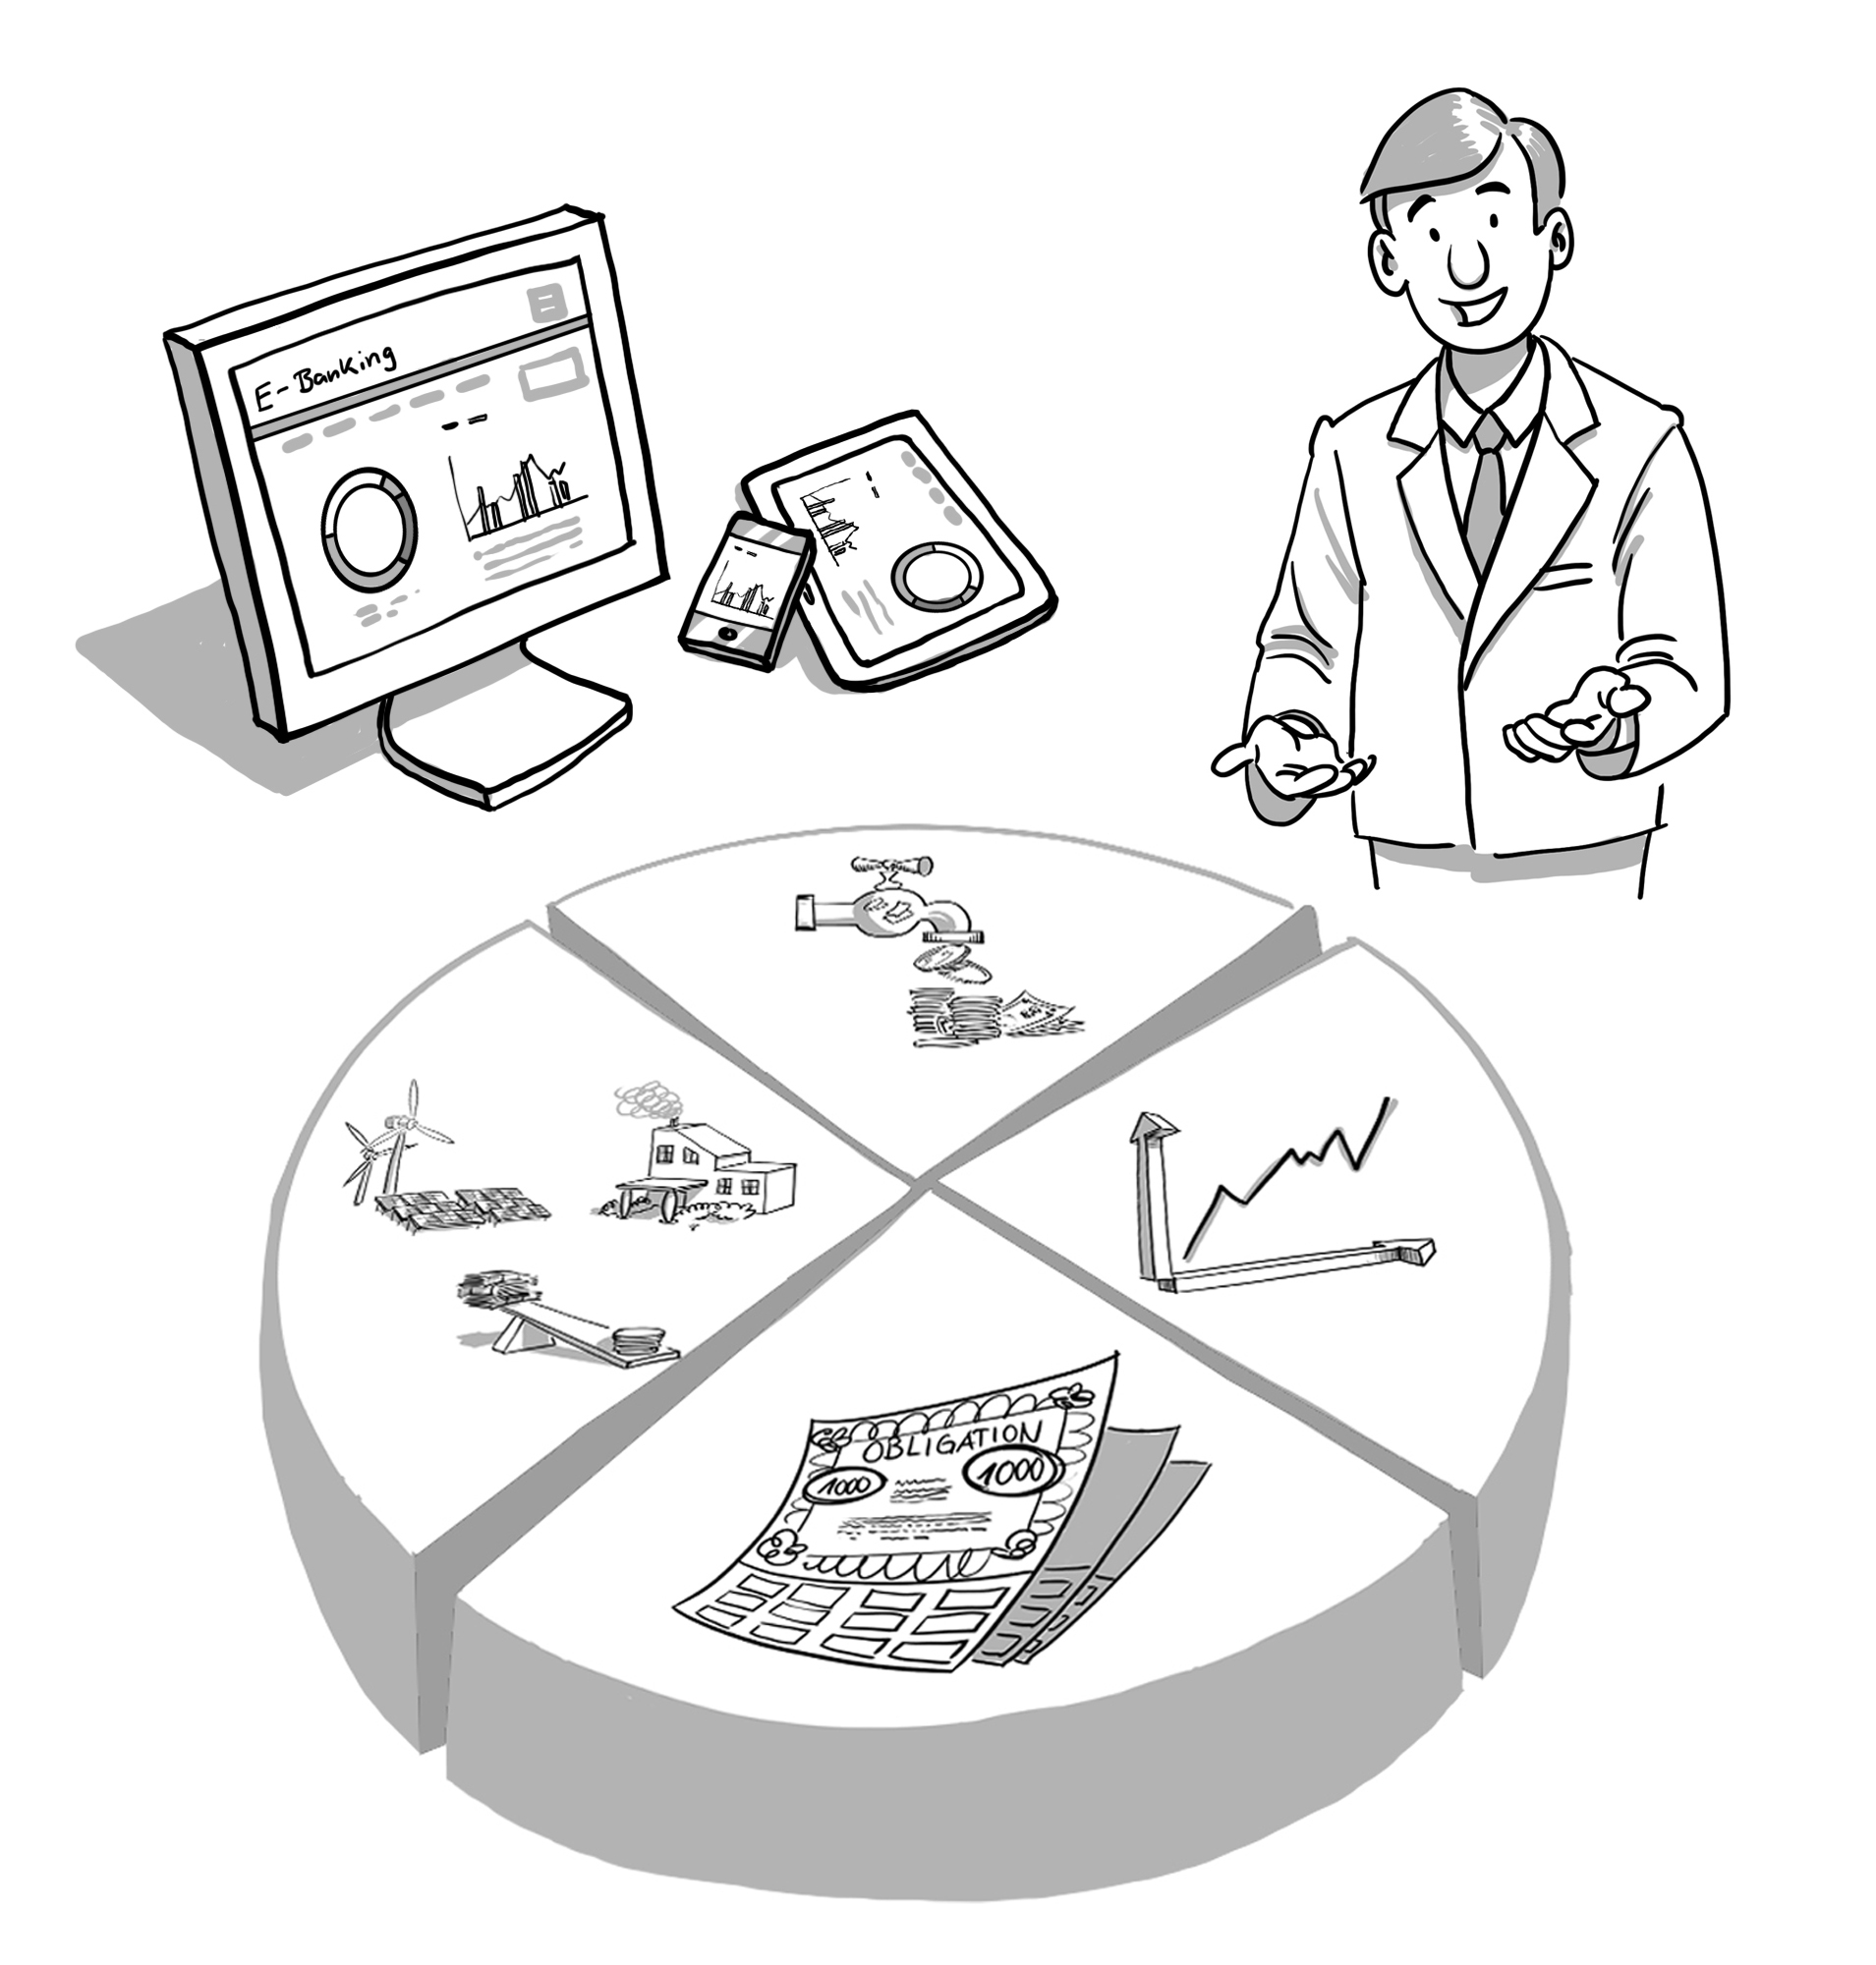
\includegraphics[scale=0.4]{img/InvestmentSolutions.jpg}
	\end{minipage}
\end{figure}

\vspace*{1\baselineskip}

\HRule \\[0.4cm]
{\LARGE \textbf{Development of the Portfolio Management Game 2.0}}
\HRule \\[1.5cm]

\vspace*{1\baselineskip}

{\large \textbf{Master Project}}

\vspace*{1\baselineskip}

\scshape % Small caps
\large University of Zurich - Department of Banking and Finance \\ \vspace{3.5mm}

\vspace*{2\baselineskip}

\textbf{Authors:} \\
\text{Roland Schlaefli - rolandschlaefli@gmail.com} \\
\text{Pascal Zehnder - pascal\_zehnder@outlook.com} \\

\vspace*{0.9\baselineskip}

\textbf{Supervisor IFI:} \\
\text{Prof. Dr. Chat Wacharamanotham} \\

\vspace*{0.9\baselineskip}

\textbf{Supervisors DBF:} \\
\text{Prof. Dr. Markus Leippold, Dr. Benjamin Wilding} \\

\endgroup
\end{titlepage}

\newpage

\pagenumbering{roman}

% ----------------------------------------
% Inhaltsübersicht
% ----------------------------------------
\tableofcontents

\newpage

% ----------------------------------------
% Start des eigentlichen Inhalts
% ----------------------------------------
\pagestyle{headings}
\pagenumbering{arabic}

\clearpage
\section{Introduction}


\clearpage
\section{Project Description}
The ''Portfolio Management Game'' was initially developed in 2001 by an external company for the Department of Banking and Finance. This simulation of a portfolio manager was being used from the DBF over several years by multiple seminars of their departement. A course named ''Advanced Portfolio Seminar'' has given insights to the portfolio management process for Master students by playing the game in between different rounds playing the game. For the final seminar of the ''Executive Education'' the game was being played for two days on Uetliberg with all the executive students.

The game has been deprecated by its implemented technologies and after each round the supervisors had to collect a USB-stick where all decisions of the students have been saved to. The supervisors had to collect this data for each group on a central device with administrative access (on a windows native application) to calculate the result of the teams decisions.


\clearpage
\section{Methodology}
\label{sec:methodology}

Different tools helped us to understand a typical investment process to model the game best for proper learning of the students, as described in \Cref{sec:introduction}. This part should give an insight into our procedure within the project.

\subsection{Requirements Engineering}
The typical requirements engineering builds the base of our engineering design process. By creating user stories we had a common basis to define the requirements together with our principals from the DBF. As usual, when defining user stories we classified those stories into the following three categories: Nice-to-have, Should-have, Must-have. Additionally, they are structured into different functional or organizational parts. All the stories can be found in the appendix~\ref{sec:appendix_user_stories}. The state of the acceptance criteria is marked in the checkboxes of the corresponding story.
% TODO more

\subsection{User Interviews}
Interviews with professionals and other people with deep knowledge of the overall process have been held to get an insight into different practices during the investment process in different companies.
\begin{itemize}
  \item Roger Burger, UBS
  \item Sandro Braun, Zürcher Kantonalbank
\end{itemize}

Both interviewers have described their job and their daily tasks, always referring to the game, as both interviewers already had played the old game. Additionally, they showed some screens of their internal applications which helped us to design the depot realization part of the student's decisions.

\subsection{Observation of Game Execution}
Besides the interviews with experts, the project team had the opportunity during summer 2018 to collect feedback within three different game executions to deepen their knowledge for an investments process and to learn about crunch points of creating a new solution. \\

Firstly, at the beginning of July, the final seminar of the Finance Executive Education took place. At this point of their study, the participants have completed most of their courses and should know the portfolio management process at least theoretically. There are also practitioners who work in the field of asset management respectively private banking. The simulation itself was played during the three days. A group of in about 30 participants played in groups of three and four. The authors had the chance to observe the groups at the beginning during their decision-making process and ask them directly for feedback. Additionally, the seminar management collected final feedbacks as well as ideas for further development at the end of the seminar, when they knew the game well, as multiple periods have been passed. \\

The second setting was set up especially for observation purposes of this project. Two students on Bachelor’s level with only basic knowledge in finance and two students on Master’s level with advanced knowledge in finance played two periods of the game in a seminar room under the observation of the authors. The main intention of this run is also to gain understanding, how players with different understanding levels of the portfolio management process would approach a decision and how a new technically implemented game will improve their play procedure. In the end, they also provided detailed feedback. \\

A third observation chance was the Master seminar ''Advanced Portfolio Management Game'' of the DBF at the beginning of September. During two seminar days, the simulation was conducted at the Swiss Bank Julius Bär. In combination with practical lectures, the students can deepen their understanding of portfolio management and present their outcomes in front of a critical jury. \\

A large number of observed students and practitioners help to gain an overview of the game process and especially from the player’s point of view obsolete or requested elements regarding the simulation. As a result of those observations and interview with students and professionals, the following work model has been defined for a typical investment process: \\

\begin{figure}[h!]
  \centering
  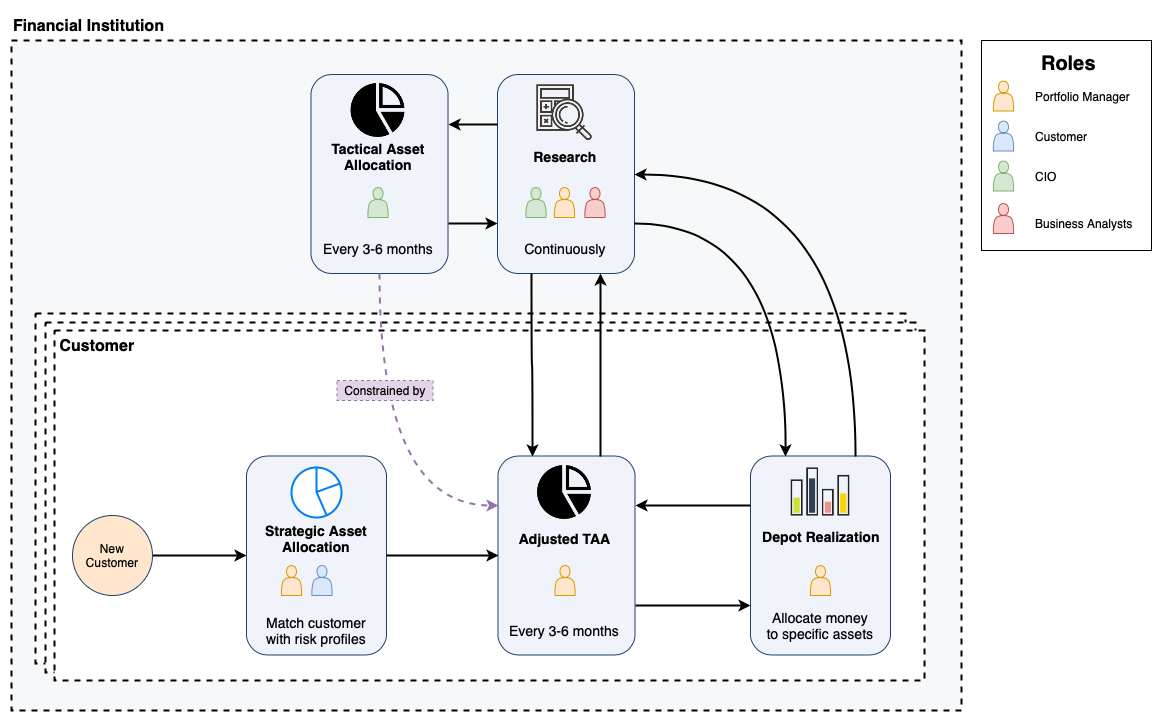
\includegraphics[scale=0.35]{img/work_model_process.png}
  \caption{Work model - global overview}
\end{figure}


Additionally, a number of relevant observations made by the authors as well as the seminar conductors and feedbacks from the participants during the three sessions are depicted – please note that in order to fully understand some of the following aspects, the reader should have seen the old version of the simulation:
\begin{itemize}
  \item \textbf{General:} Generally, the participants enjoyed playing the game and regard it as helpful to deepen their theoretical knowledge for example from the lecture ''Asset Management: Investments'' for Bachelor students. However, they regard the system as outdated and provided the authors with various ideas and critics. Decision data for a starting period 0 will be filled out by participants in Excel for a starting position before the seminar, afterward, they will be saved onto the USB drives for all teams by the seminar conductors. The seminar conductors will let the market model run and save its outcome back on the USB drive. This process is time-consuming and error-prone. In general, the participants think that it is difficult to make a decision in the first round, as too few information is available. More easily accessible comparative figures for the previous year would be helpful. Additionally, the stock selection is based on insufficient knowledge about the different titles.
  \item \textbf{Investment Process:} The given and to be kept bandwidths for the different asset class positions are not optimally placed and have to be looked up frequently. A temporary over-investment during the decision process is not possible and is always disturbed by pop-up windows.
  \item \textbf{Business Administration:} Various decisions regarding marketing, human resources as well as logistics are not very clear as especially in the beginning, the background and previous period information are not completely clear for the participants. The point here is, that a suitable level of abstraction has to be chosen as on the one hand, not every decision that has to be made in reality can be implemented in such a simplified simulation. On the one hand, a suitable number of decisions have to be enabled in order to support an appropriate learning effect.
  \item \textbf{Report:} The reports provided after each round of the game load very slowly and the comparison to other teams is cumbersome. It would be helpful if not only one group member can have the simulation and the reports on their screen. In general, more graphics are desired for better visualization of key aspects.
  \item \textbf{Teamwork:} The enabling of collaboration on several laptops within a team was mentioned many times. With today’s web-based technologies, much more implementation options are available.
\end{itemize}

The observation of the different players – students and practitioners, investment beginners and experts – allowed the project team to sense, what the strengths and weaknesses of the old game are. Further, it helped to define an impact direction for the new game being developed, which resulted in another work model describing the process of the game based on its different phases. % TODO more about customer types etc.

\begin{figure}[h!]
  \centering
  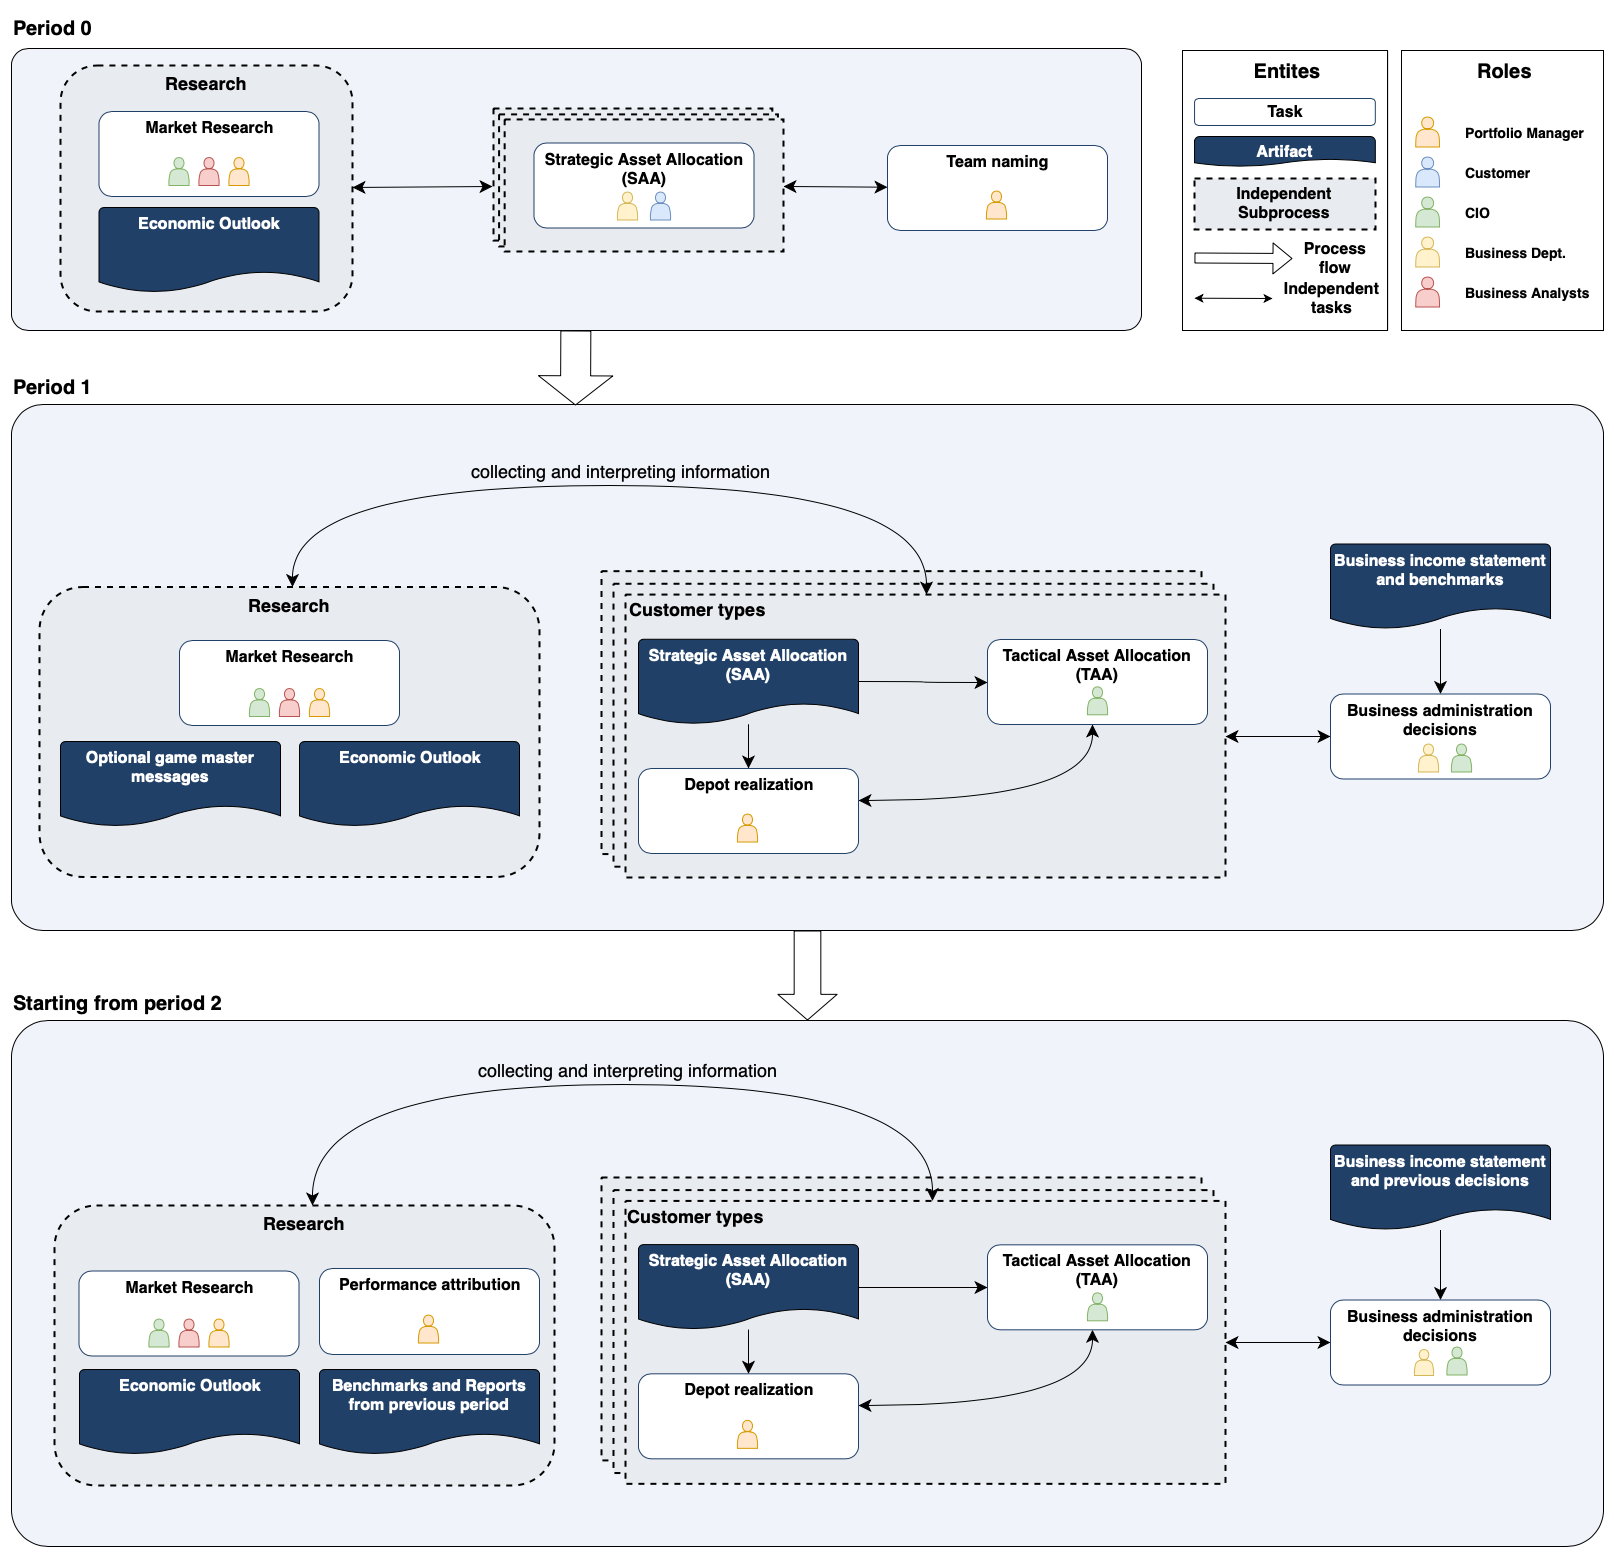
\includegraphics[scale=0.25]{img/work_model_pfm_game.png}
  \caption{Work model - portfolio management game}
\end{figure}

\subsection{Design and Iterative Prototyping}
Initially, the authors designed multiple screens based on the predefined work model. Using a sketching software the basic screens for the student's process which includes the SAA, TAA, depot realization and business administration were prototyped. As the team realized that the game does not only consist of screens from a student perspective they decided, due to time constraints, to start implementing screens by iterative prototyping. \\

Multiple concepts had to be defined, such as how to model the game session management. By defining a timeline the administrative user always gets a direct response of the state of the game. This colorful timeline builds the base of the game detail screen, while other visualizations or forms depending on the state of the game.\\

Another big concept was defining the process of the student's input. The process is depicted on the top located game navigation bar on the right corner. Each processing task (SAA, TAA, depot realization, business administration) has its own progress state. Different concepts have been tried to model this process best intuitive for the users.
% TODO more?


\clearpage
\section{Architecture}

\begin{center}
  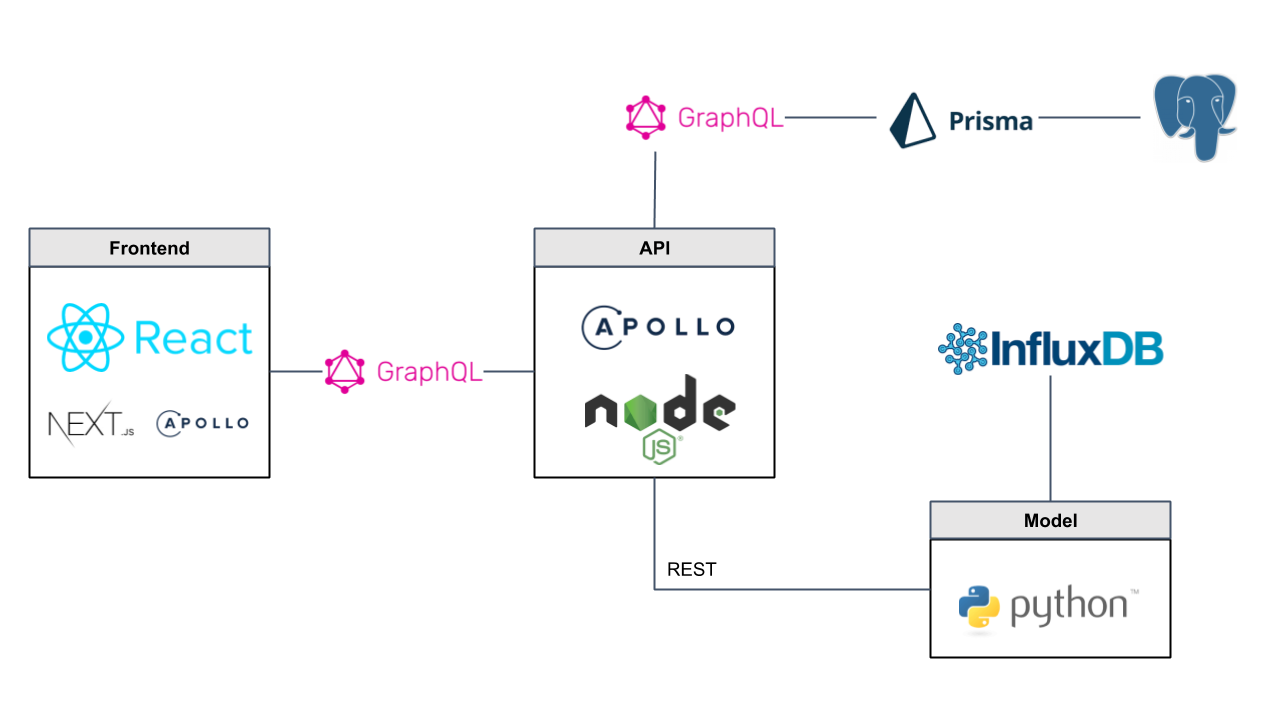
\includegraphics[scale=0.45]{img/architecture.png}
\end{center}

\subsection{Frontend}
We use the React Framework which is developed by Facebook. Based on NextJS.

\subsection{API}
Bla


\subsection{Model}
All calculations of the simulation are performed in a python-model which interacts with the time series data stored on an InfluxDB. A Restful service fetches the data from the model.

\subsection{Contnious development}


\clearpage
\section{Market Model}

\begin{figure}[h!]
  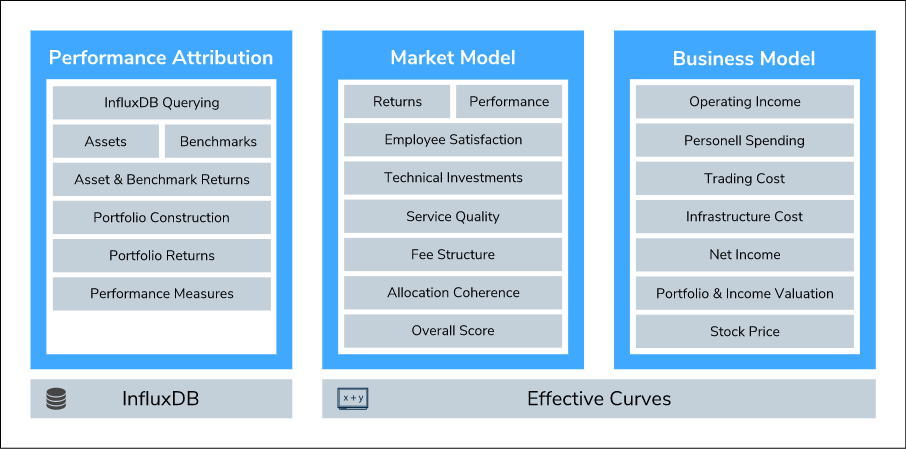
\includegraphics[width=\textwidth]{img/market_model.png}
  \caption{Market Model Overview}
  \centering
  \label{fig:market_model_overview}
\end{figure}

The PFM-Game market model is a module that produces period results based on the business decisions and portfolio allocations of teams participating in a given game. The market model is separated into several subcomponents that, when applied in sequence, produce results for a period of the game.

\subsection{Data and Data Ingestion}
The underlying data driving all portfolio-related calculations in the market model is comprised of several hunderd time-series that are stored in InfluxDB. The majority of these time-series describe asset price or return indices (i.e., asset prices normalized by the payment of dividends and other interest) as extracted from the Thomson Reuters Datastream platform. Further relevant time-series are based on macroeconomic data extracted from the FRED (Federal Reserve Economic Data) database. These data are used to calculate portfolio and benchmark returns as well as parameters of an economic forecast.

The above described data can be extracted from Datastream and FRED and ingested into an instance of InfluxDB automatically by means of a Python module that was created as an extension to the PFM-Simulation project. Data to be ingested is defined inside an assets.csv file in the following CSV format:

\begin{table}[h!]
  \begin{tabular}{lllllll}
    \toprule
    Name & Symbol  & Start Date & Market      & Data Type & Asset Type & Currency \\
    \midrule
    SWISS BOND AAA & SWBND3A & 29.12.2006 & Switzerland & RI        & BONDS      & CHF      \\
    NESTLE 'R'     & S:NESN  & 01.01.1973 & Switzerland & RI        & EQUITY     & CHF      \\
    \bottomrule
  \end{tabular}
  \centering
  \caption{Exemplary assets in a valid assets.csv definition format (optional columns omitted)}
  \label{table:assets_csv}
\end{table}

During processing of the CSV definition of all assets, the module will incrementally extend existing time-series with new data up to the current day. Time-series that were not previously available will be stored as a new series in full-length.


\subsection{Performance Attribution}
The performance attribution module is the first module in the sequence of model calculations that are applied to an incoming period scoring request (i.e., a request made by the game master on completion of a game period).

% modules/performance_attribution/influx.py
\subsubsection{InfluxDB Querying}
As can be seen in \ref{fig:market_model_overview}, one of the most important responsibilities of the performance attribution module is handling all data querying from the InfluxDB time-series database. Based on the incoming depot allocations of all participating teams, the module fetches all necessary asset and benchmark values from the database.\footnote{See pfm-model/api/modules/performance\_attribution/influx.py}

% modules/performance_attribution/returns.py
\subsubsection{Asset \& Benchmark Returns}
For all of these extracted time-series, returns need to be calculated in order to be able to continue with portfolio construction steps. All computations later in the sequence will be based on these relative return measures and not on any absolute values of the time-series.\footnote{See pfm-model/api/modules/performance\_attribution/returns.py}

% modules/performance_attribution/portfolio.py
\subsubsection{Portfolio Construction}
With returns being available for all assets and their benchmarks, the performance attribution module then constructs portfolios for each team. Each team will have created one portfolio allocation for each customer type that is enabled in the current period. The module will account for this by building as many portfolios per team as there are customer types.\footnote{See pfm-model/api/modules/performance\_attribution/portfolio.py}

In addition to building portfolios for all depot allocations of the current period, the performance attribution module also computes one benchmark portfolio for each asset portfolio. These benchmark portfolios are based on the strategic asset allocation of the corresponding customer type. As the strategic asset allocation is defined once per game during period zero, the composition of these benchmark portfolios will stay the same. Only their returns will change, as the time-frame played changes with each period.

% modules/performance_attribution/returns.py
\subsubsection{Portfolio Returns}
Once portfolios are built for each combination of teams and active customer types, returns need to be calculated in the same way that returns were calculated for the assets previously. However, these returns need to be additionaly weighted by the amount of money that has been invested into each asset. For example, if a team were to invest 10\% of their total assets under management in one asset and 20\% in another, the latter would influence the overall portfolio returns twice as much as the former.

% modules/performance_attribution/kpi.py
\subsubsection{Performance Measures}
Upon completion of all previous returns calculations, the returns of assets, benchmarks, and portfolios can be combined into many useful performance measures that characterize a portfolio in different ways and allow for an easier intercomparison between teams. A byproduct of these calculations is also the new assets under management for a customer given their portfolio returns, as well as the new asset positions that a portfolio is composed of after returns are applied.For example, if one invested 50\% in one asset and 50\% in another, the new positions after returns might be 45\%-55\% if the latter asset outperforms the former.\footnote{See pfm-model/api/modules/performance\_attribution/kpi.py}

% TODO: measure list in appendix
The calculated portfolio measures include measures like the selection and tactical performance attribution that can show how much an investment into a specific asset, asset type, or market benefitted the overall portfolio. A list of all calculated measures can be found in TODO: APPENDIX. These measures could then be used by the teams to reevaluate their investments.

The final results of the performance attribution module are compiled into a suitable format and passed on to the market model module, which handles the integration of these results with business decisions as well as the grading of performance measures according to efficient curves.


\subsection{Market Model}
The market model module is the second module in the sequence of calculations and builds upon the results of the performance attribution module. It ingests these results as well as business decisions of all teams and performs several grading procedures based on all of these data. The final output of the module are several index and subindex values that, e.g., describe the employee satisfaction or the overall team score on a range from 0 to 10.

As the market model is comprised of quite a lot of calculation steps and formulas, we will not go deeply into technical specifics. Instead, we briefly describe the overall structure of the module and its main subcomponents as well as how the underlying effective curves (i.e., formulas) can be parametrized.

\subsubsection{Effective Curves}
To facilitate the grading of arbitrary values on a scale of zero to ten and allow for additional parametrization, formulas that we call effective curves are applied. These formulas most often follow the general schema of computing the market average and, based on a comparison with specific portfolio-related values (\(\Delta = value - value_{avg}\)), calculating a positive or negative deviation from a base value (e.g., \(5 + \Delta \)).

An simple example for an effective curve could be:
\[\text{index value} = 5 + \frac{\Delta}{20000}\]

where the value would be constrained to lie in \([0, 10]\). More complex variants apply different functions based on the domain of the delta value. For example, the full returns index is computed as follows (if the delta value is positive):
\[\text{returns index} = 5 + \log(1 + 10 * |(return - return_{avg}) * 100|)\]

If the delta were negative, the result of the logarithm would simply be inverted to its negative value.

\subsubsection{Overview of Computed Indices}
The market model encompasses many calculations and intermediary values. \ref{fig:market_model_dependencies} shows the dependencies and interconnections between all these values, as well as how the final score index and number of customers are calculated.

\begin{figure}[h!]
  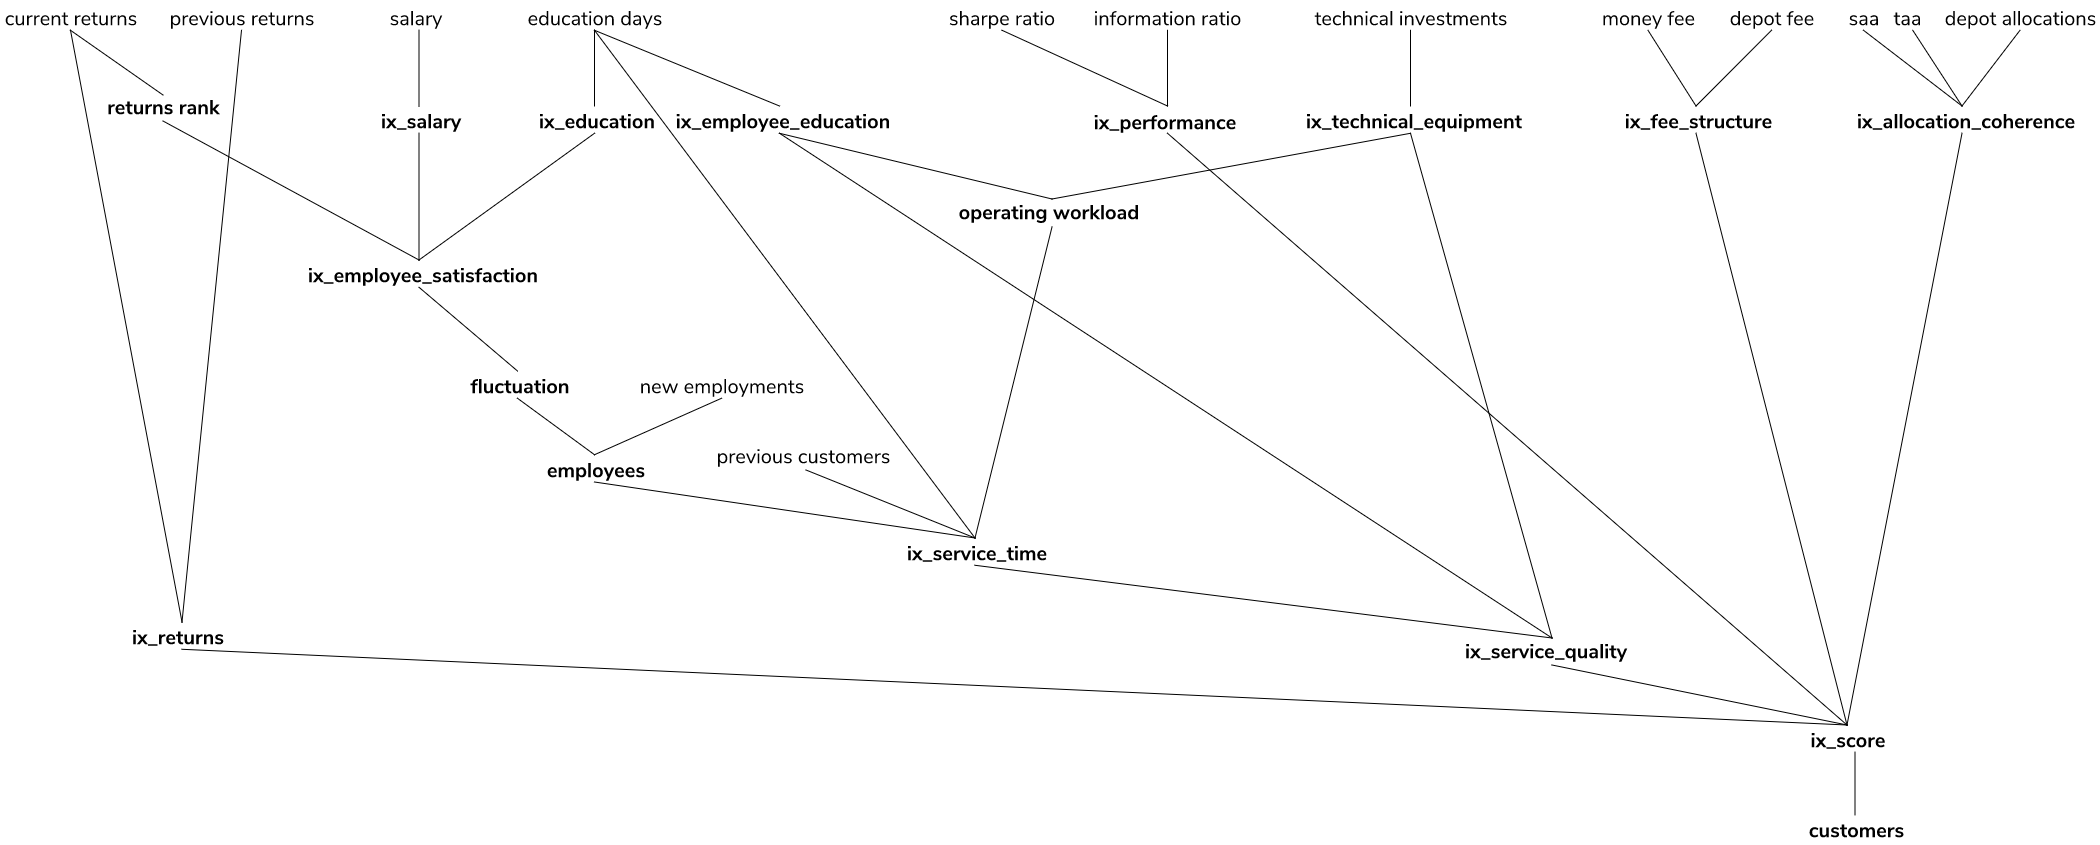
\includegraphics[width=\textwidth]{img/market_model_dependencies.png}
  \caption{Market Model Dependencies}
  \centering
  \label{fig:market_model_dependencies}
\end{figure}

\begin{table}[h!]
  \begin{tabular}{lp{11cm}}
    \toprule
    Name & Description \\
    \midrule
    ix\_returns & How portfolio returns compare against competitors \\
    \midrule
    ix\_sharpe\_ratio & How well the sharpe ratio compares against competitors \\
    ix\_information\_ratio & How the information ratio compares against competitors \\
    ix\_performance & Combination of performance indices \\
    \midrule
    ix\_salary & How satisfied employees are with their salary \\
    ix\_education & How satisfied employees are with their education \\
    ix\_employee\_satisfaction & How satisfied the employees are with overall working conditions \\
    \midrule
    ix\_employee\_education & How much employee education boosts efficiency \\
    ix\_technical\_equipment & How appropriate the IT infrastructure is after depreciation  \\
      ix\_service\_time & How appropriate the time spent for customer service is perceived \\
    ix\_service\_quality & How well overall customer service is perceived \\
    \midrule
    ix\_fee\_structure & How well the all-in management fee is perceived \\
    \midrule
    ix\_allocation\_coherence & Number of SAA violations and relative TAA discrepancy \\
    \midrule
    ix\_score & Combination of all indices into an overall rating \\
    \bottomrule
  \end{tabular}
  \centering
  \caption{Description of all indices calculated in the market model module}
  \label{table:market_model_indices}
\end{table}




\subsection{Business Model}



\subsection{API Specification}


\clearpage
\section{Application Overview}
For playing a game, an administrator of a specified game and an infinite number of teams have to interact together and compete against each other. This section should give an overview about functionalities of the game, as well as introducing the reader about crunch points in the sense of creating an intuitive user interface.

\subsection{Administration}
All administrative tasks will be described in this part to provide a game for the students which is supported well by the game master. An administrator may supervise multiple games in one account and the games could be played simultaneously.

\subsubsection{Administrator login}
An administrator needs to have a login for having all these administrative functionalities. Therefore he has to provide his credentials on the following screen which he reaches by following the instructions on the start page. By entering his game master credentials, the administrator will be redirected to the game overview (Paragraph~\ref{paragraph:game_overview}).
\begin{figure}[h!]
  \centering
  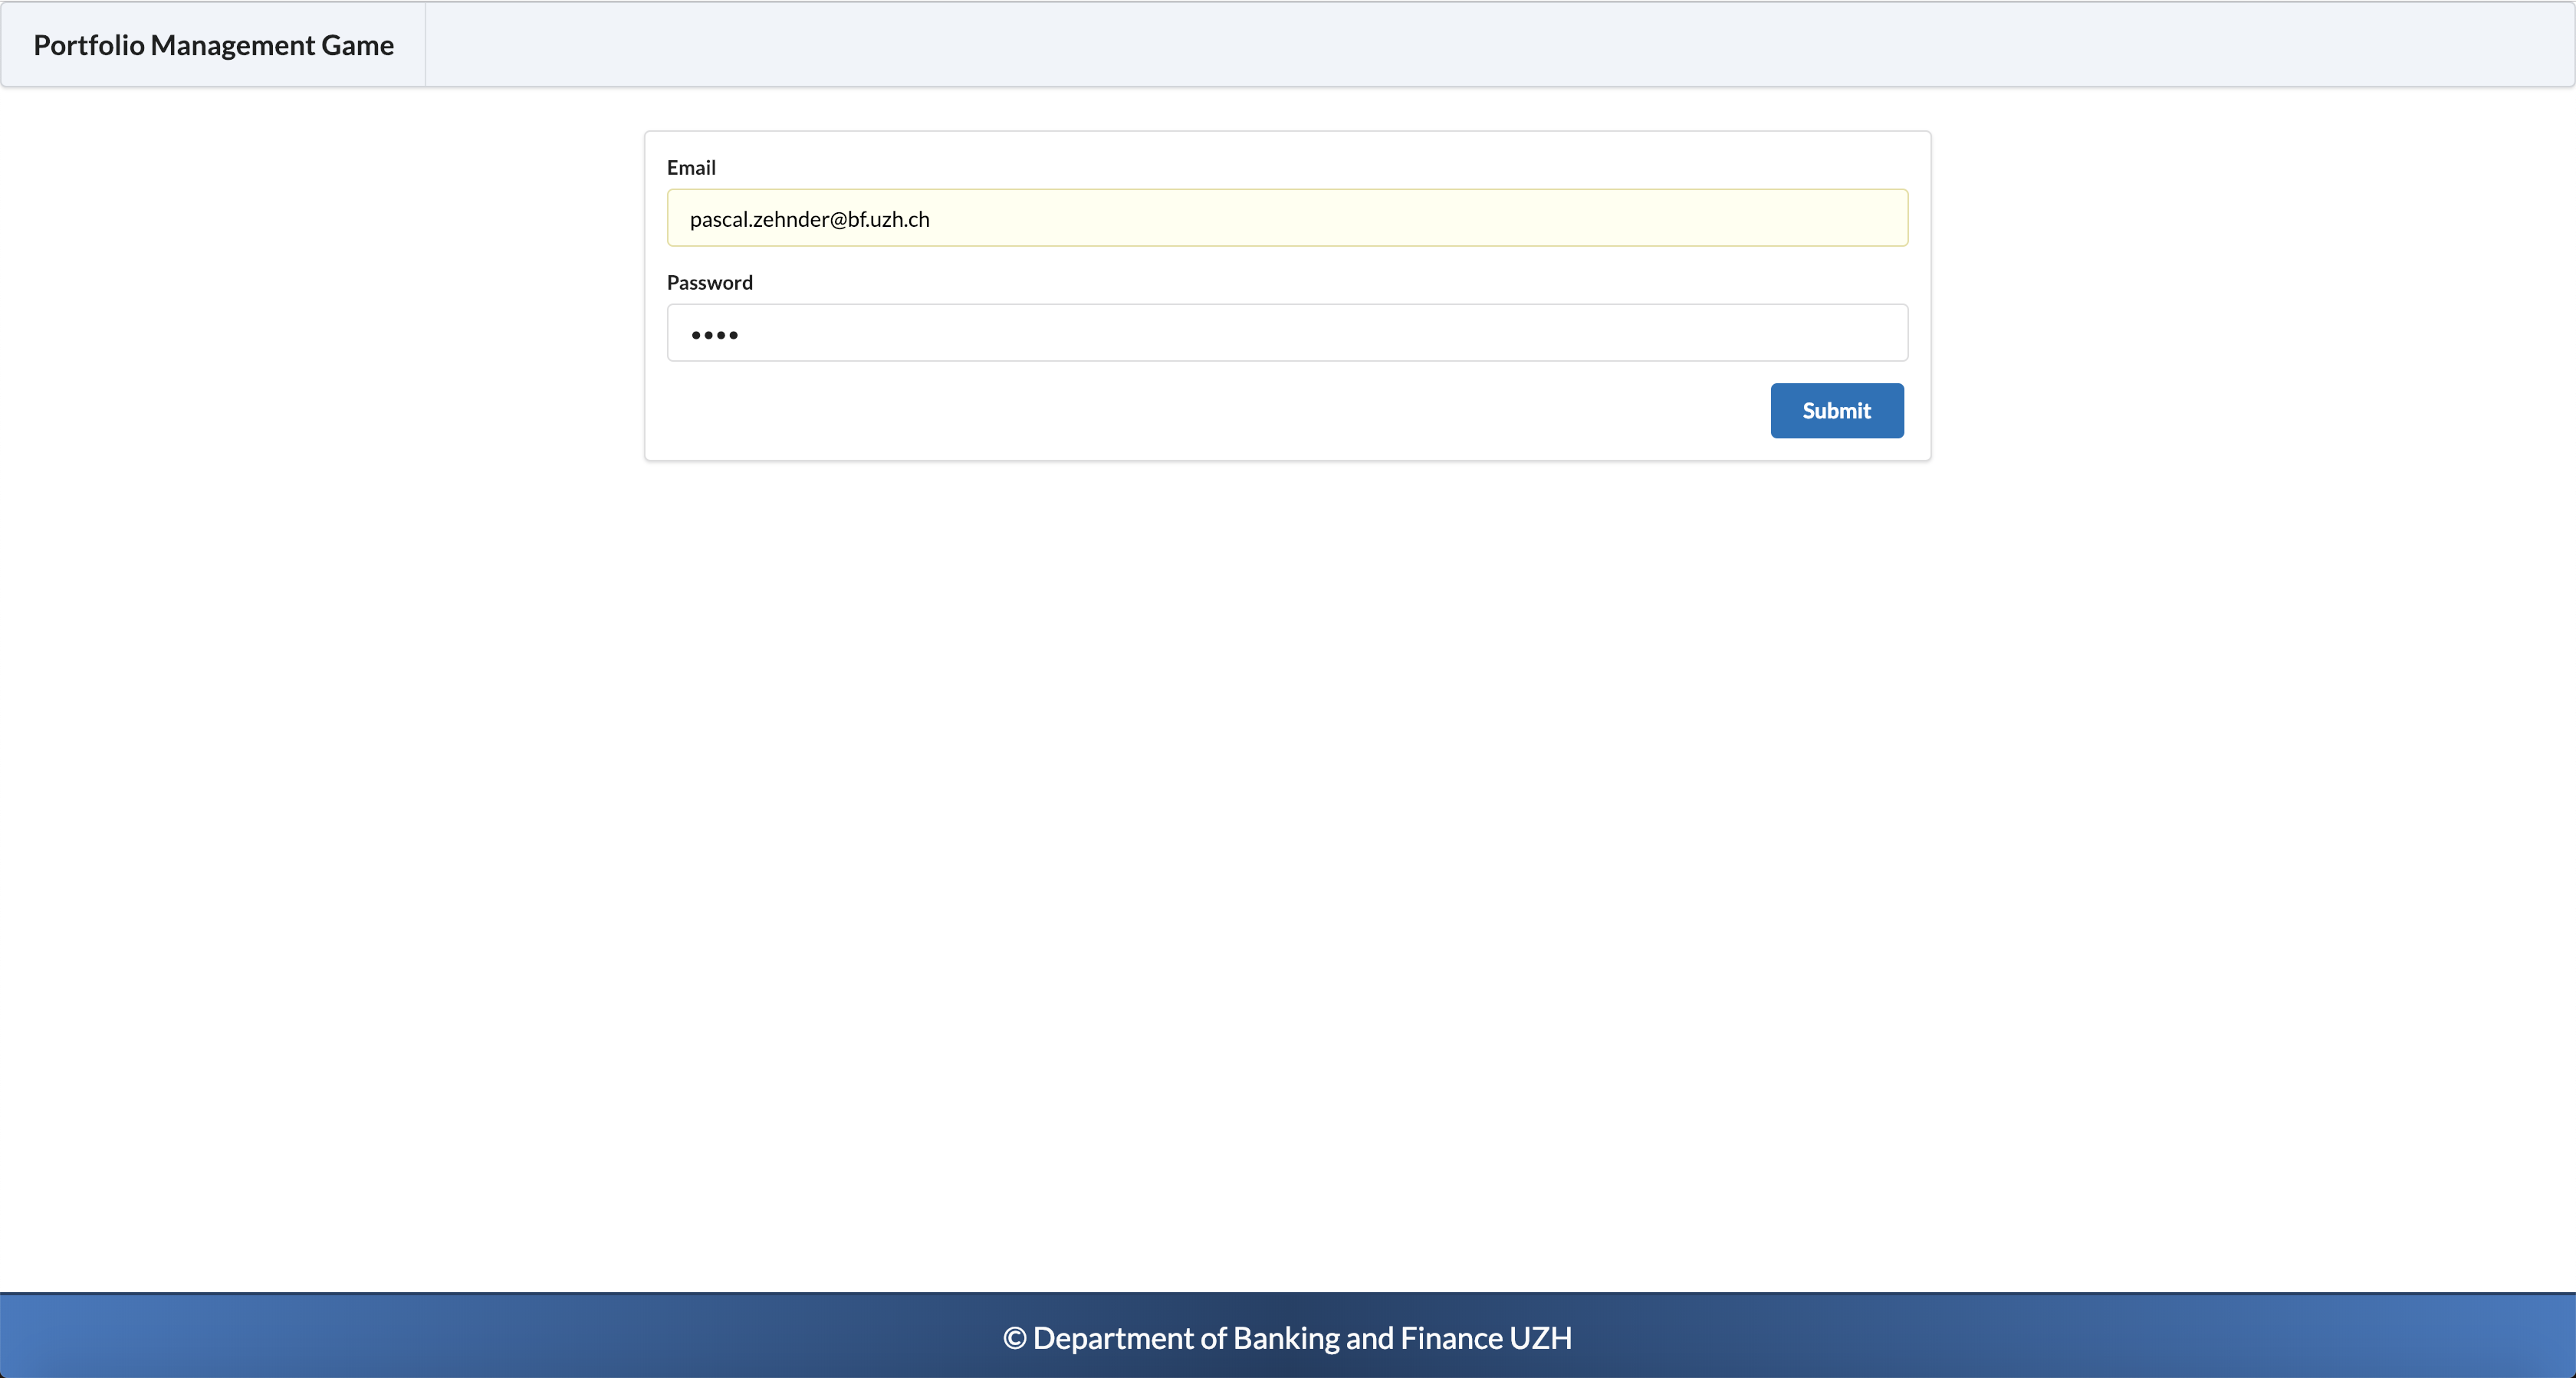
\includegraphics[scale=0.2]{img/application-overview/administrator/01_login.png}
  \caption{Administrator login}
\end{figure}

\subsubsection{Game management}
\paragraph{Game overview}
\label{paragraph:game_overview}
As for landing page of the administrator the game overview exists. It serves as the control center of the game administration. Multiple games can be maintained simultaneously by one game master. Some instant information identifies the current progress of the game within the list, such as game name, short game id or the phase of the game.
\begin{figure}[h!]
  \centering
  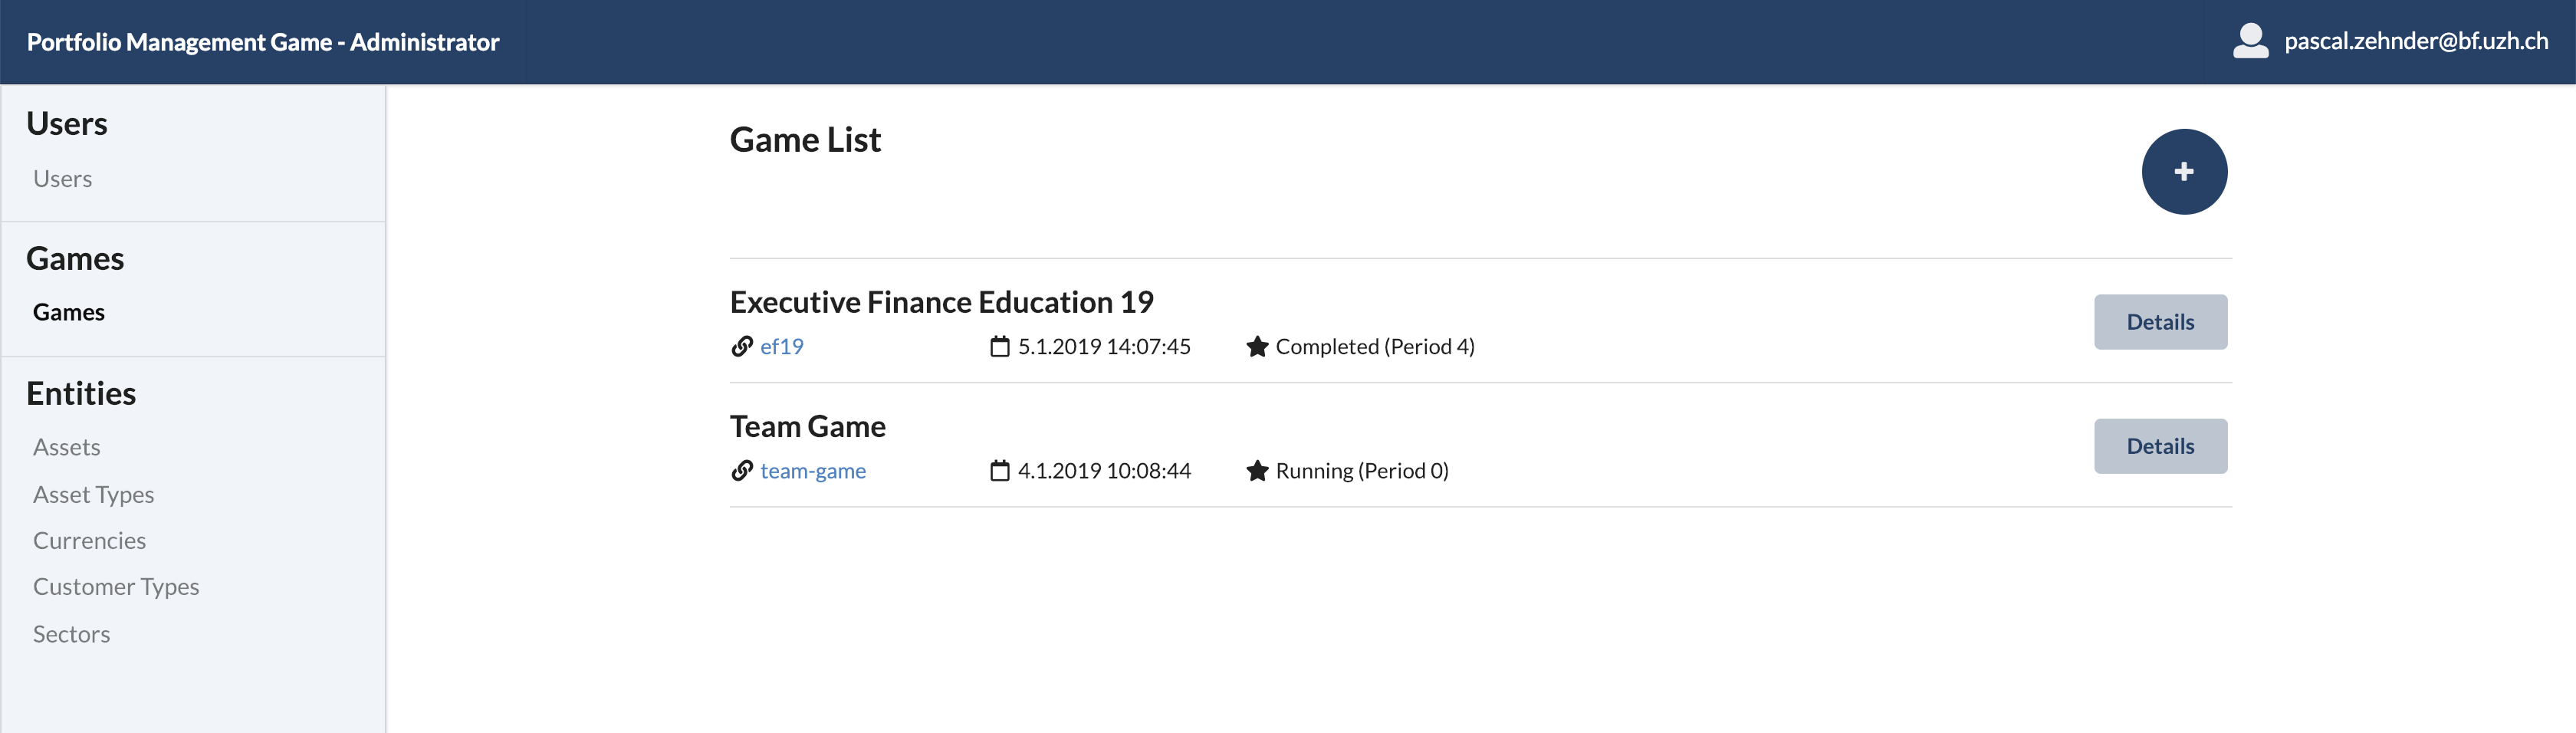
\includegraphics[scale=0.2]{img/application-overview/administrator/02_game_overview.png}
  \caption{Game overview}
  \label{fig:game_overview}
\end{figure}

\paragraph{Game creation}
For creating a game the administrator needs to define some parameters, by filling out a form which is structured into three steps. By pressing on the ''next''-button the administrator will be led through the form. Some tooltips help users to understand the purpose of the provided input. After submitting the creation of the game, the user will be redirected to the game detail of the newly created game.
\begin{figure}[h!]
  \centering
  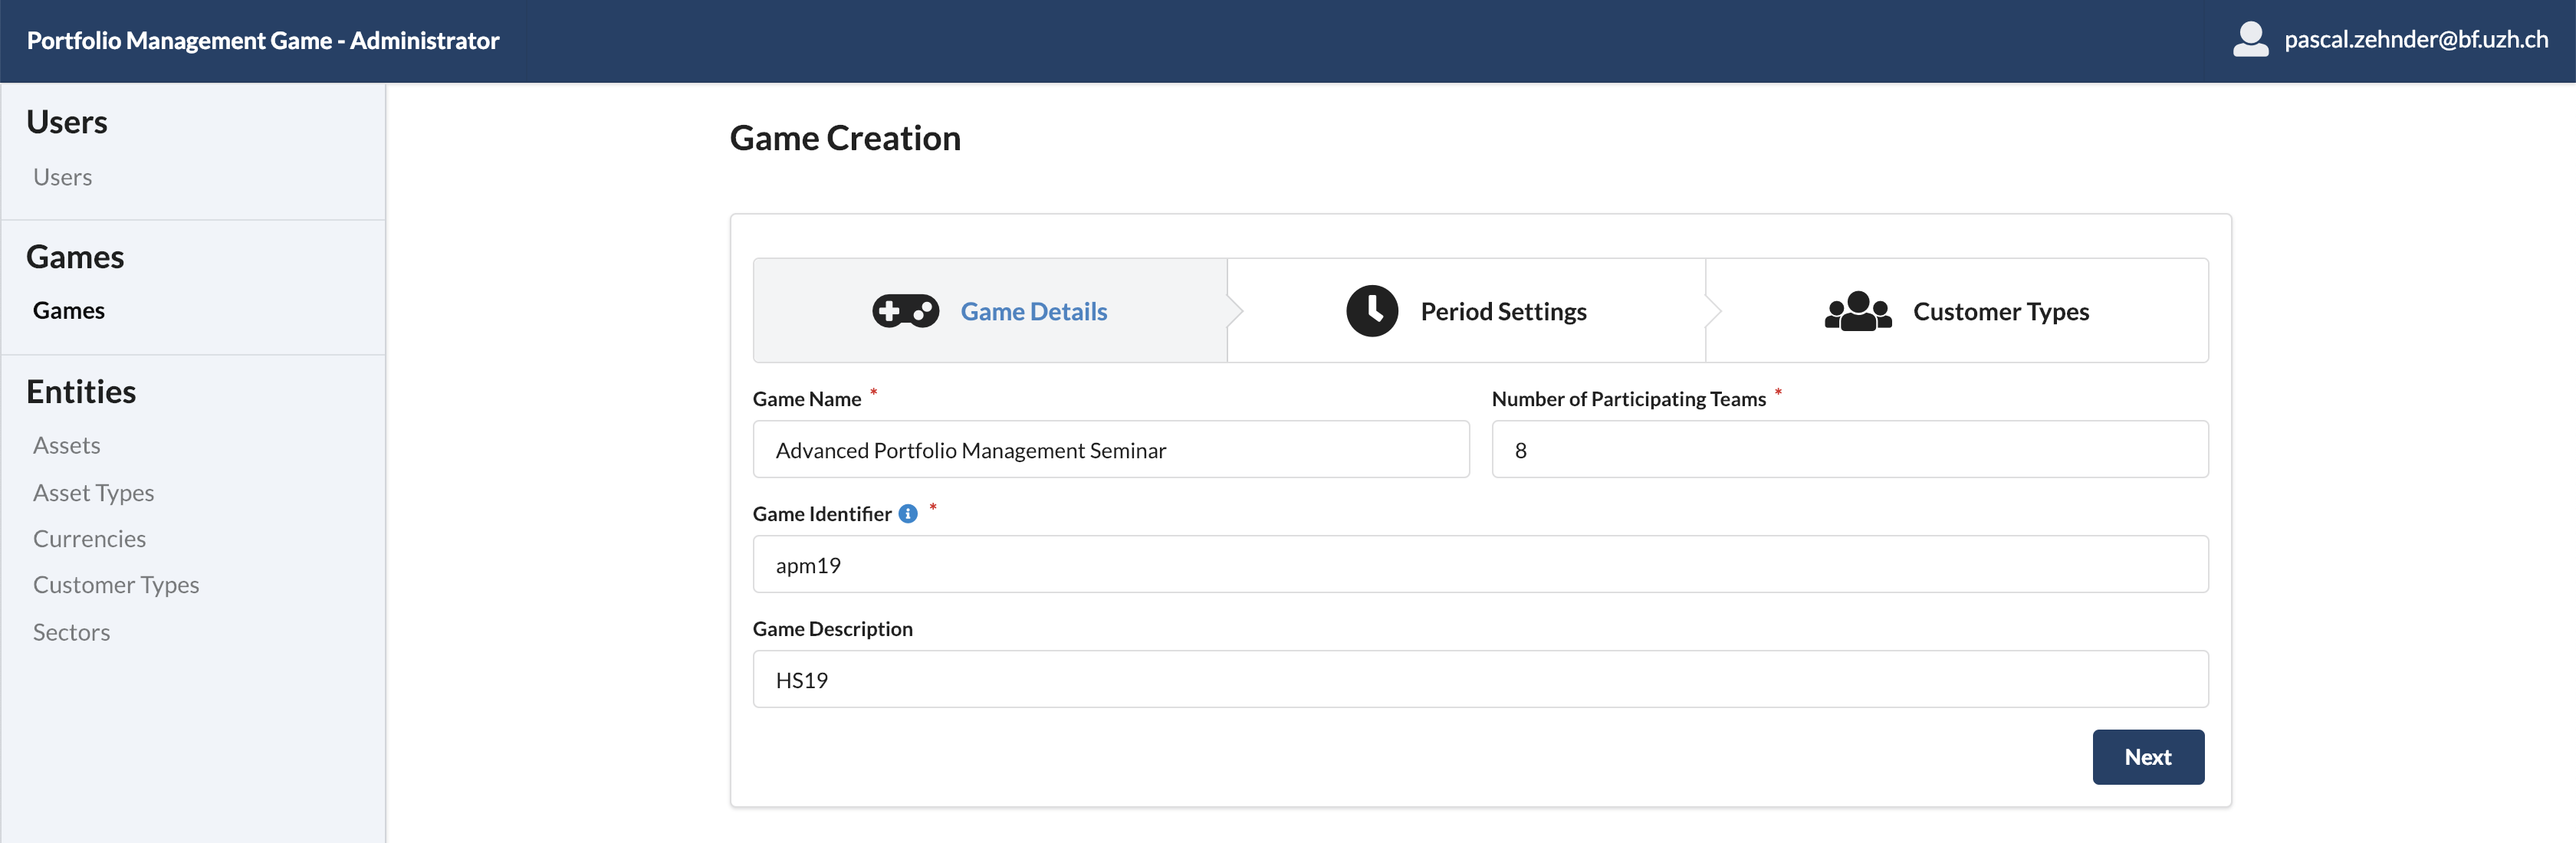
\includegraphics[scale=0.2]{img/application-overview/administrator/03_game_creation.png}
  \caption{Game creation}
\end{figure}


\paragraph{Game detail}
The game detail for each game may be accessed over the game overview list, as seen in figure~\ref{fig:game_overview}. In this page a user can initialize period, start periods, have an overview of the teams' submission and many other features, which will be described in this paragraph:

\subparagraph{Game initialization}
As the game creation may be done in advance we have split the game creation from the game initialization, such that last adjustments of the game may be done just before the start of the game.
\begin{figure}[h!]
  \centering
  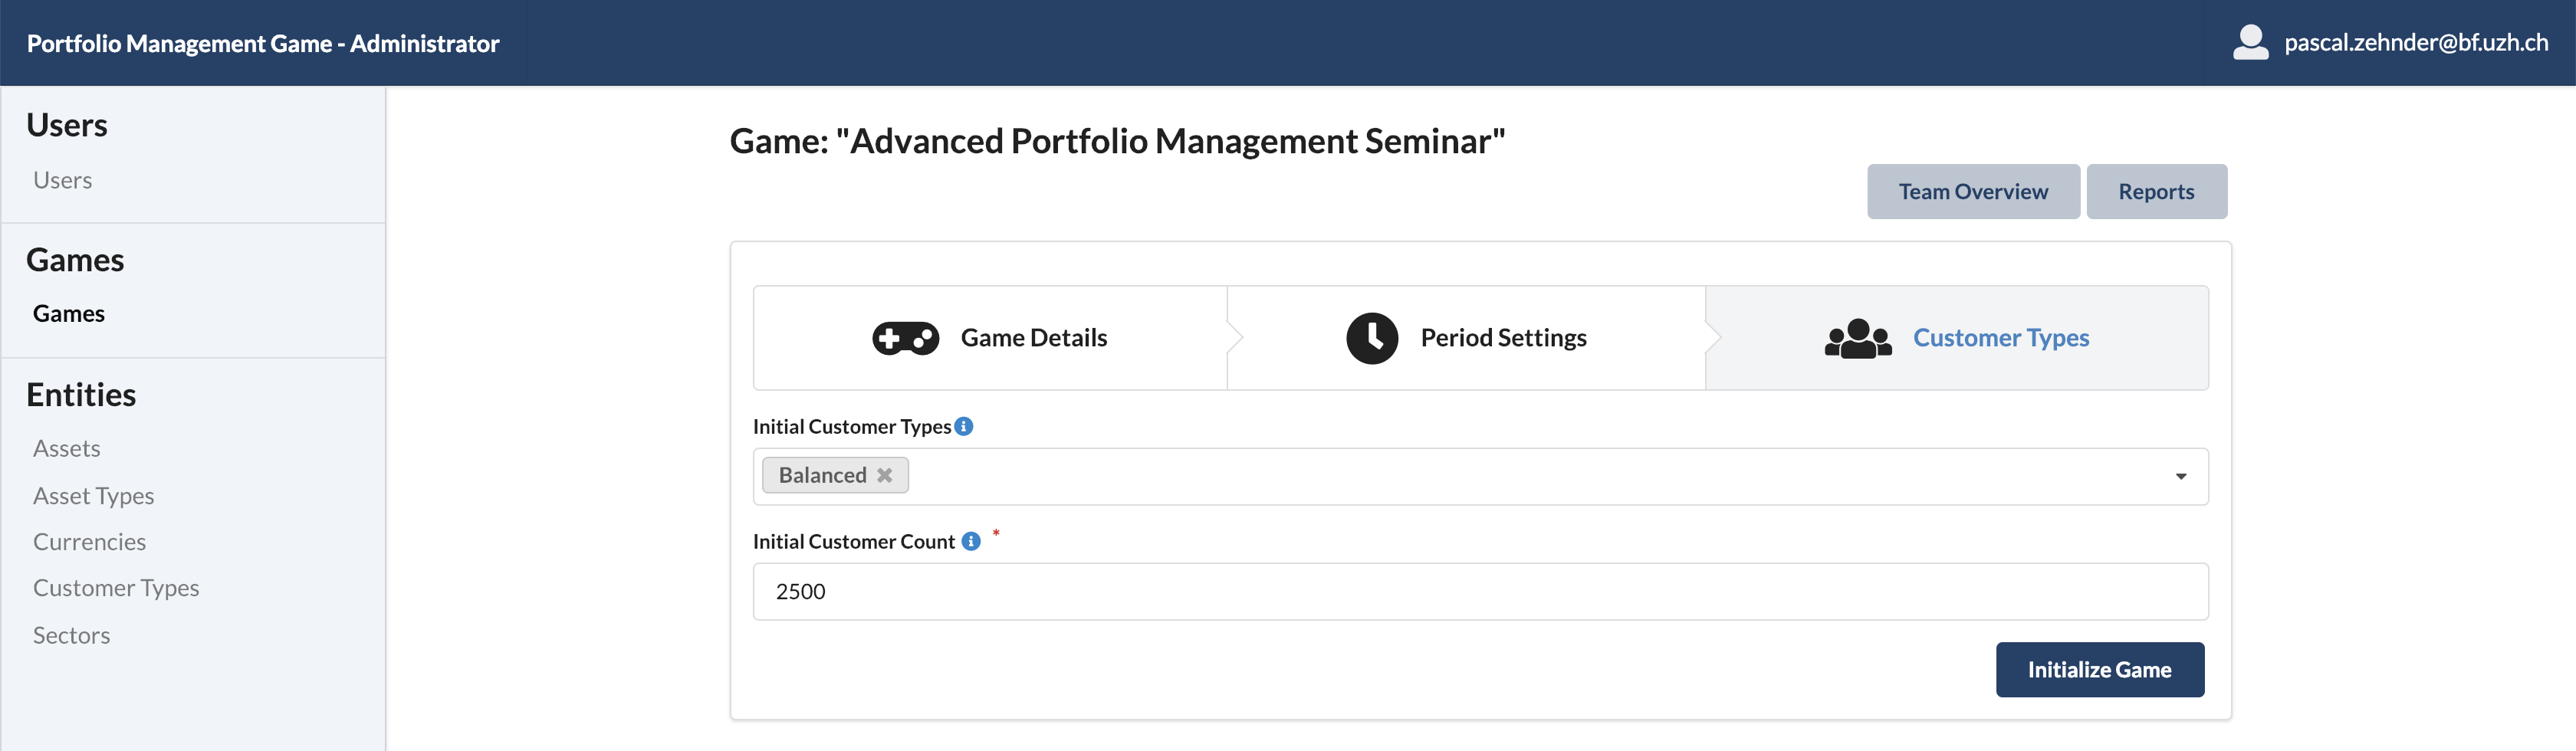
\includegraphics[scale=0.2]{img/application-overview/administrator/04_game_initialization.png}
  \caption{Game initialization}
\end{figure}

\subparagraph{Game start}
By starting the game the students or teams are finally able to start with their period zero decisions. Administrators are able to give them some help over messages which will be visible for the teams in their report section by creating customizable messages. Figure~\ref{fig:game_start} shows a game which is still planned and may be started next.
\begin{figure}[h!]
  \centering
  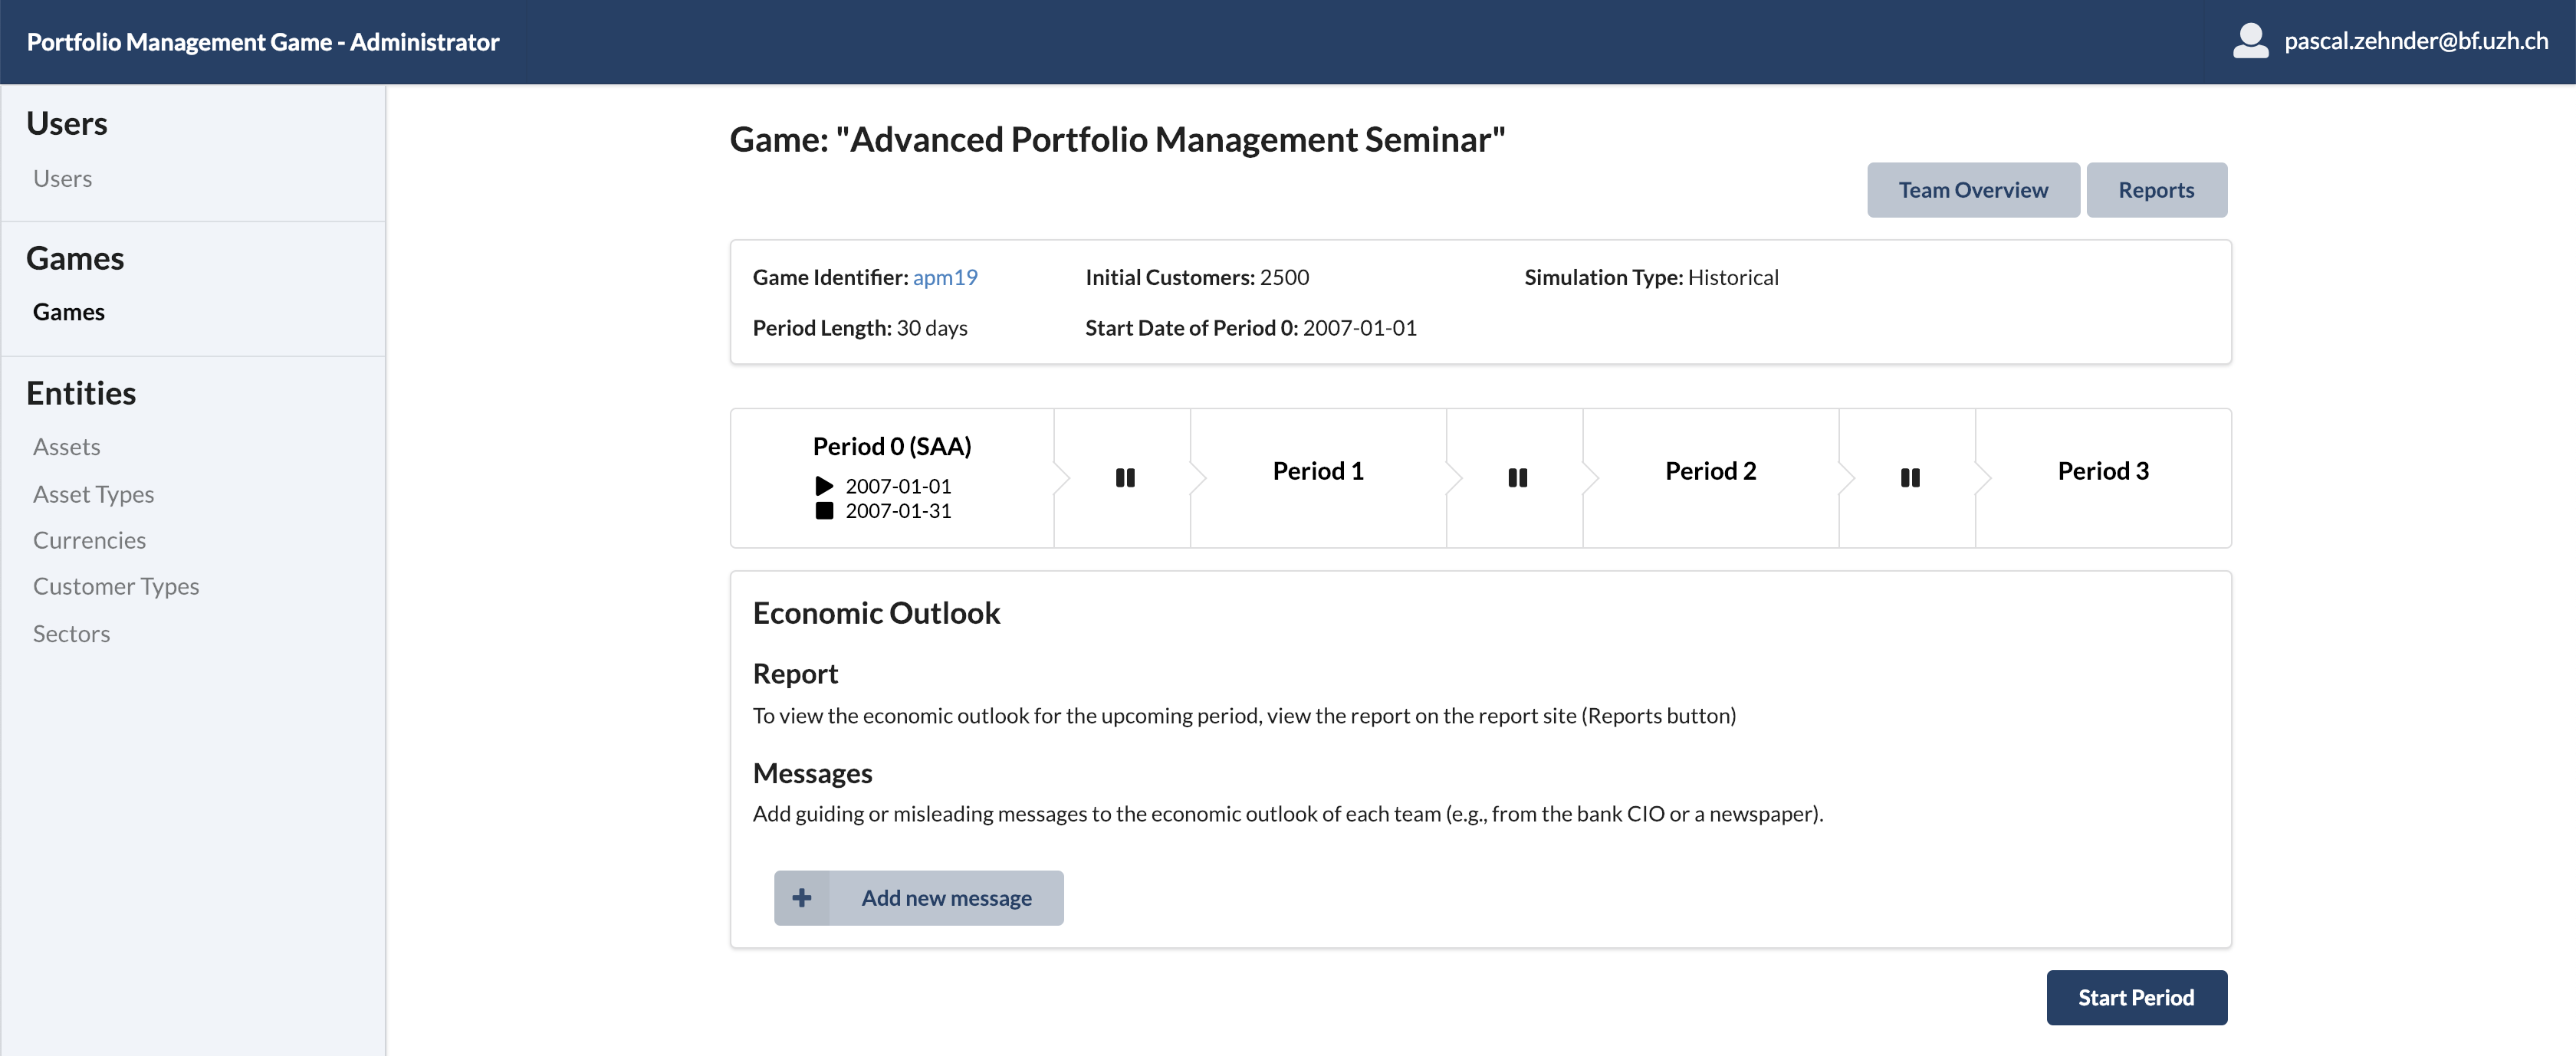
\includegraphics[scale=0.2]{img/application-overview/administrator/05_game_start.png}
  \caption{Game start}
  \label{fig:game_start}
\end{figure}


\subparagraph{Team overview}
\label{subparagraph:team_overview}
For providing access for all teams an administrator has an overview about the team logins (figure~\ref{fig:team_overview}), which are generated automatically when initializing a game.
\begin{figure}[h!]
  \centering
  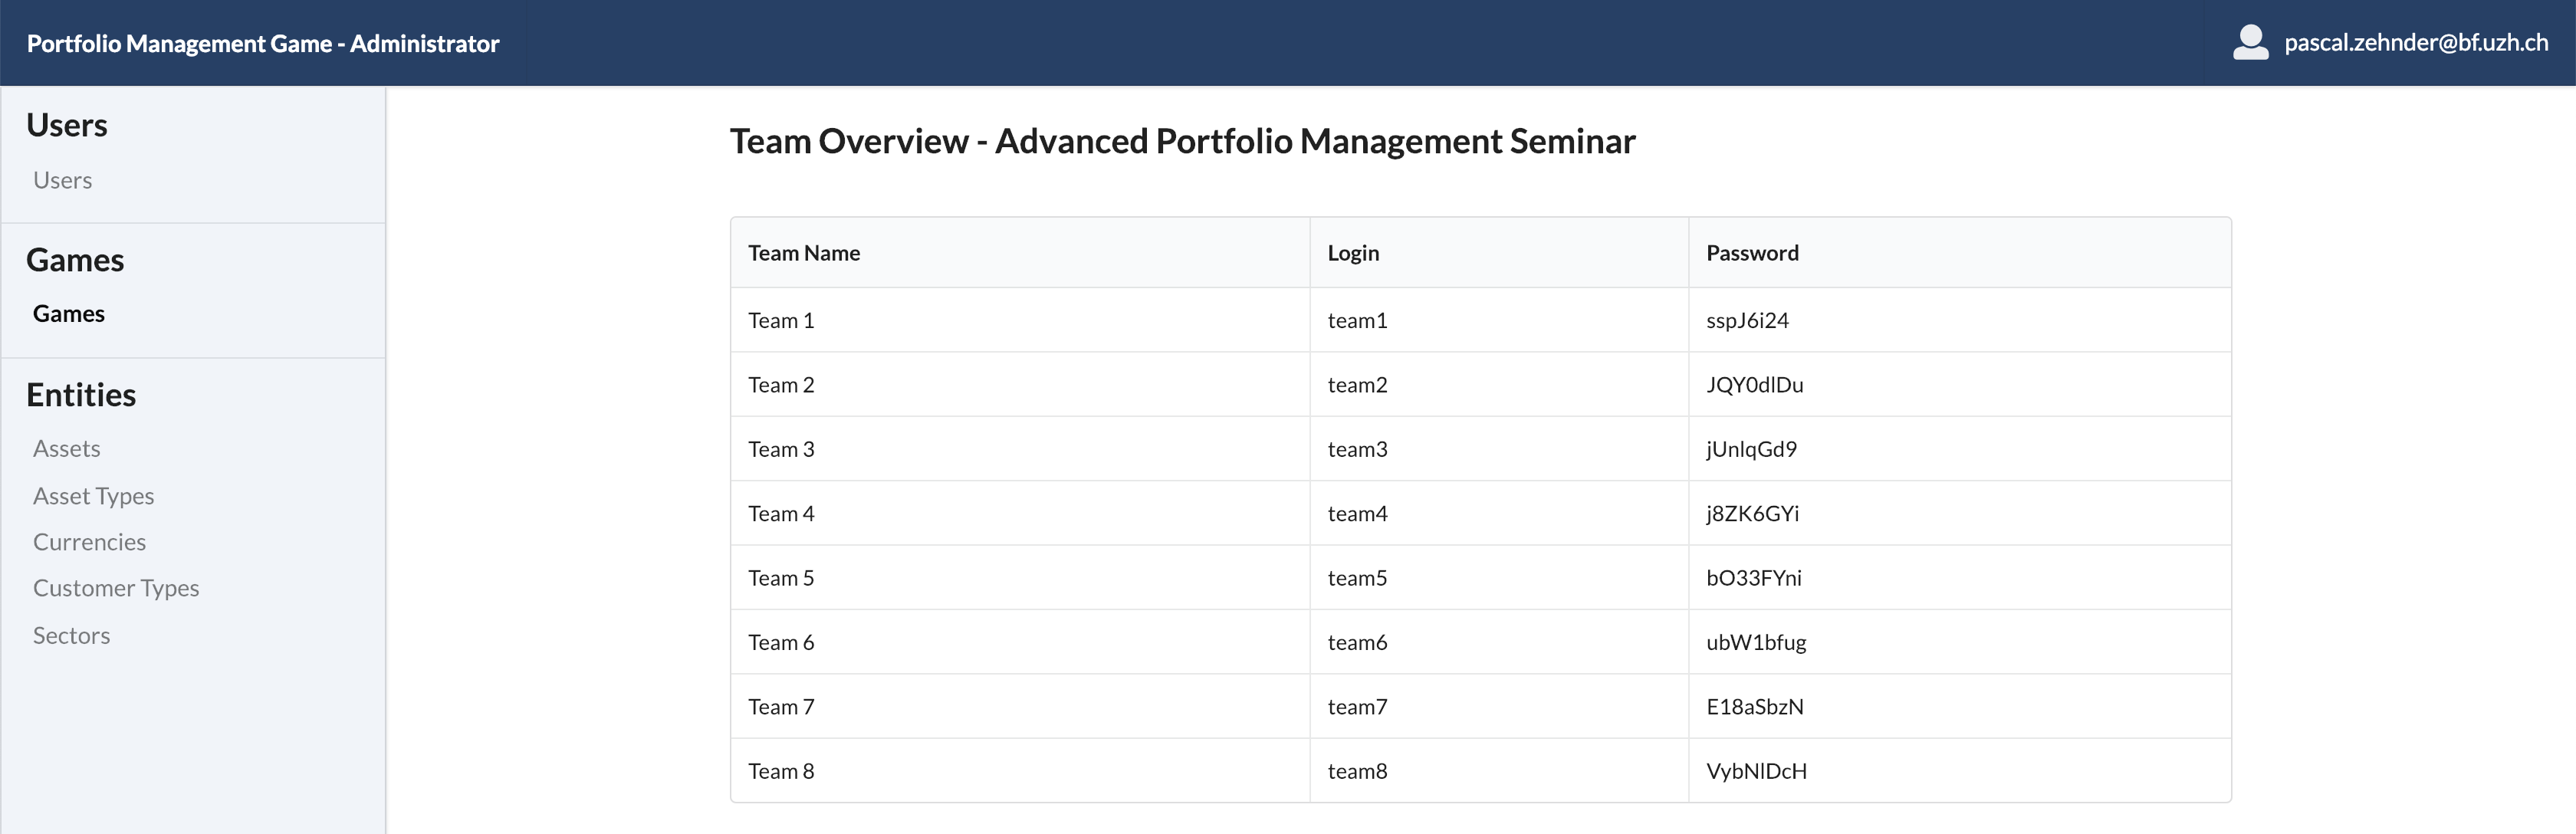
\includegraphics[scale=0.2]{img/application-overview/administrator/06_team_login_overview.png}
  \caption{Team overview}
  \label{fig:team_overview}
\end{figure}

\subparagraph{Running game}
Overview of the submission state of all teams. The administrator is able to get an insight about the decisions of all submitted teams. The period can only be finished if all teams submitted and therefore the state of the teams has been green.
\begin{figure}[h!]
  \centering
  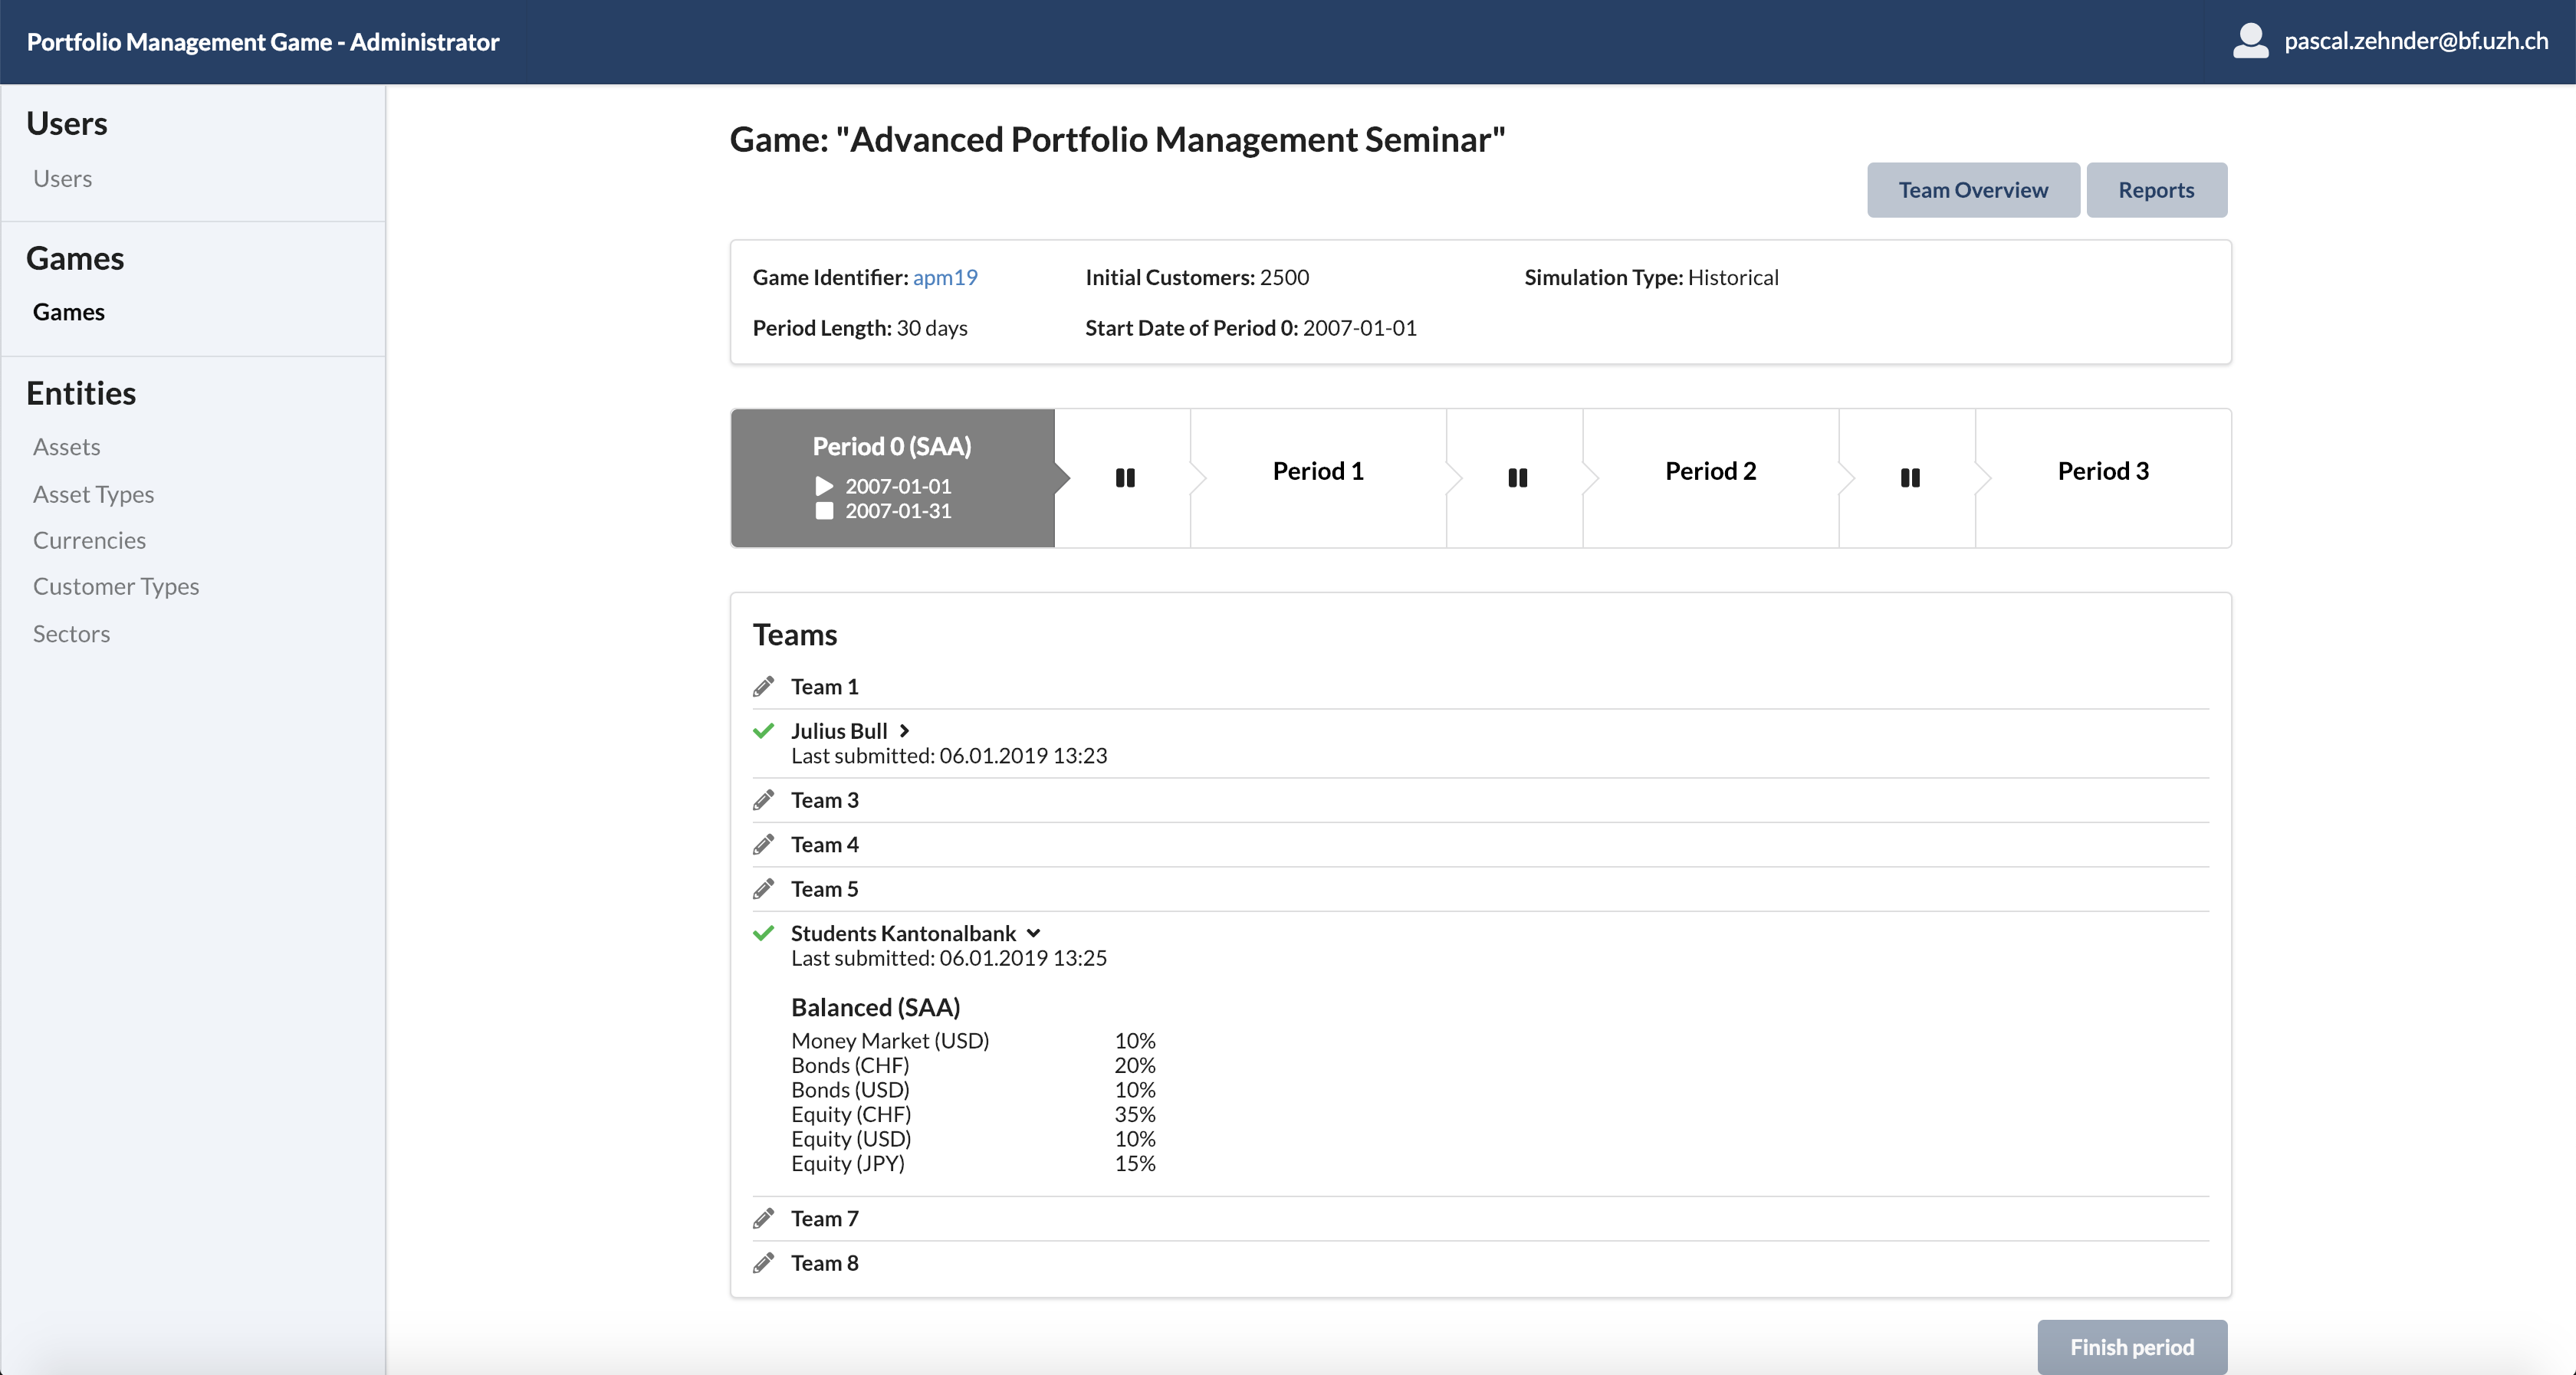
\includegraphics[scale=0.2]{img/application-overview/administrator/07_running_game.png}
  \caption{Running game}
\end{figure}

\subparagraph{Initializing period}
After completion of period zero, the administrator has to initialize a period in which the team decisions will be compared to the other teams decisions and evaluated. Additionally, new customer types for the next period and other settings could be defined in this phase of the game.
% TODO replace with a screen including customer type settings from period 2 e.g.
\begin{figure}[h!]
  \centering
  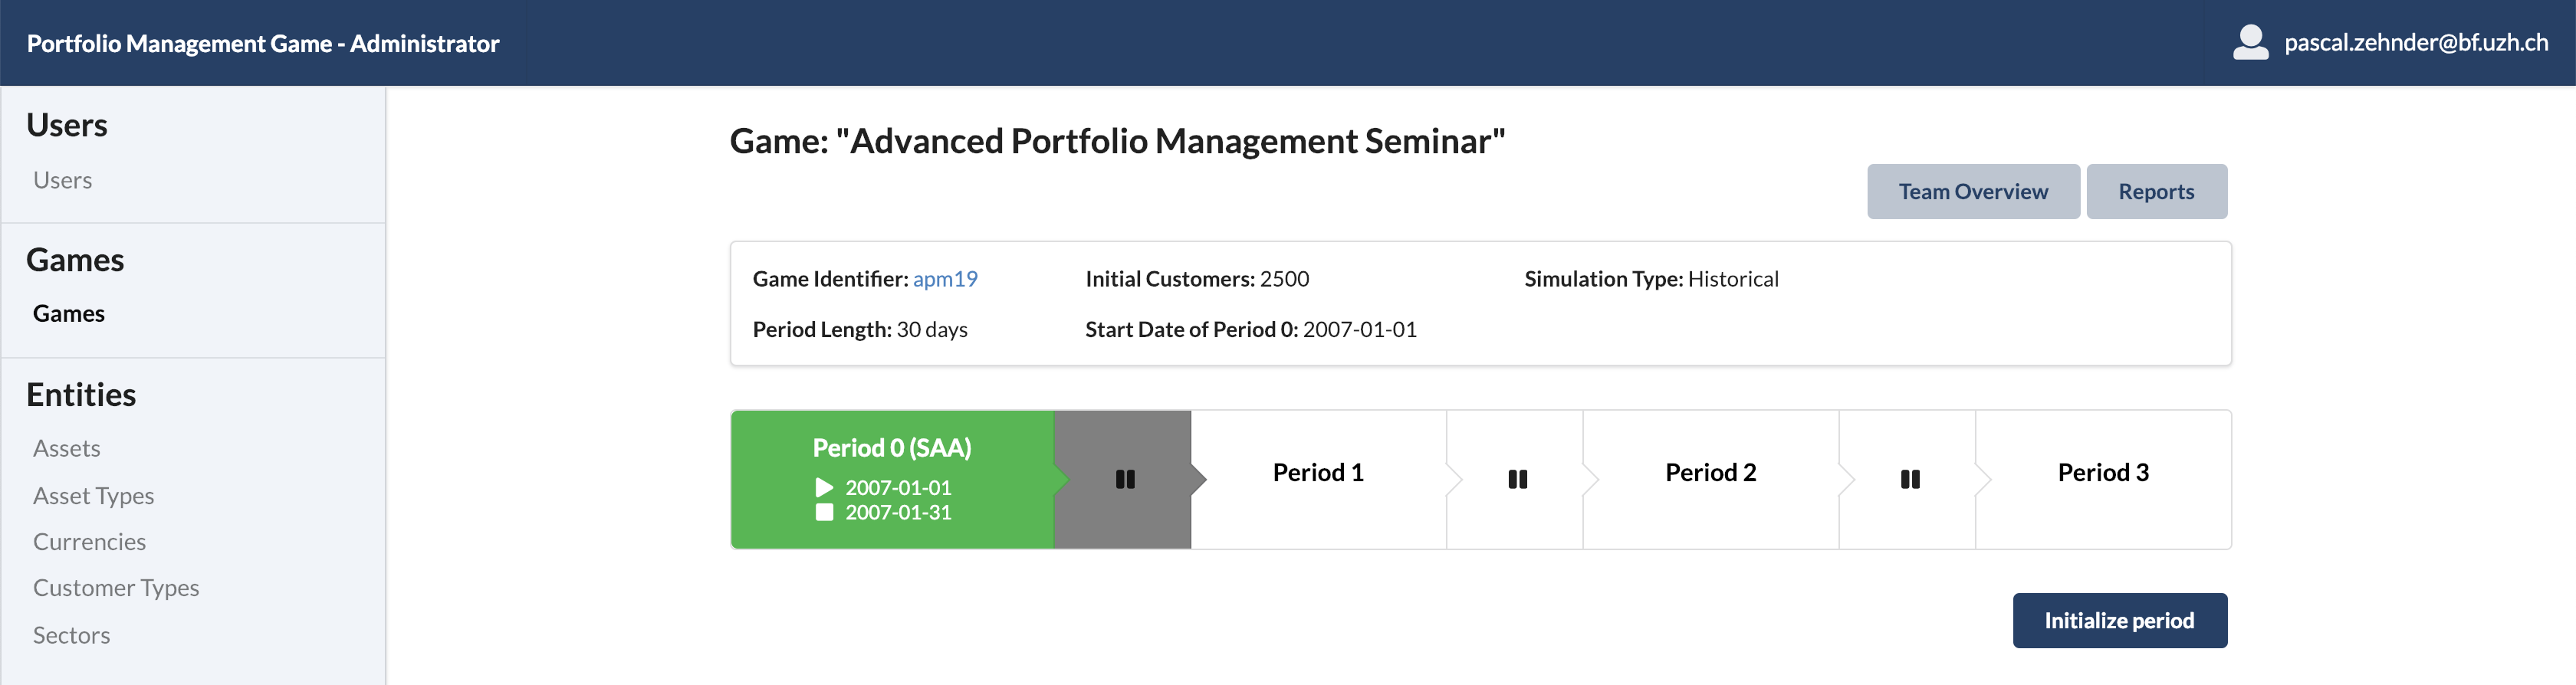
\includegraphics[scale=0.2]{img/application-overview/administrator/08_period_initialization.png}
  \caption{Initialize period}
\end{figure}


\subparagraph{Period start}
By completing the simulation, respectively evaluation of the previous period, a next period may be started. If the game is still paused the teams cannot access the decisions site. The administrator can define some optional messages which will be displayed in the teams report page. Some adjustments to the simulation results will be edited in this phase of the game.
\begin{figure}[h!]
  \centering
  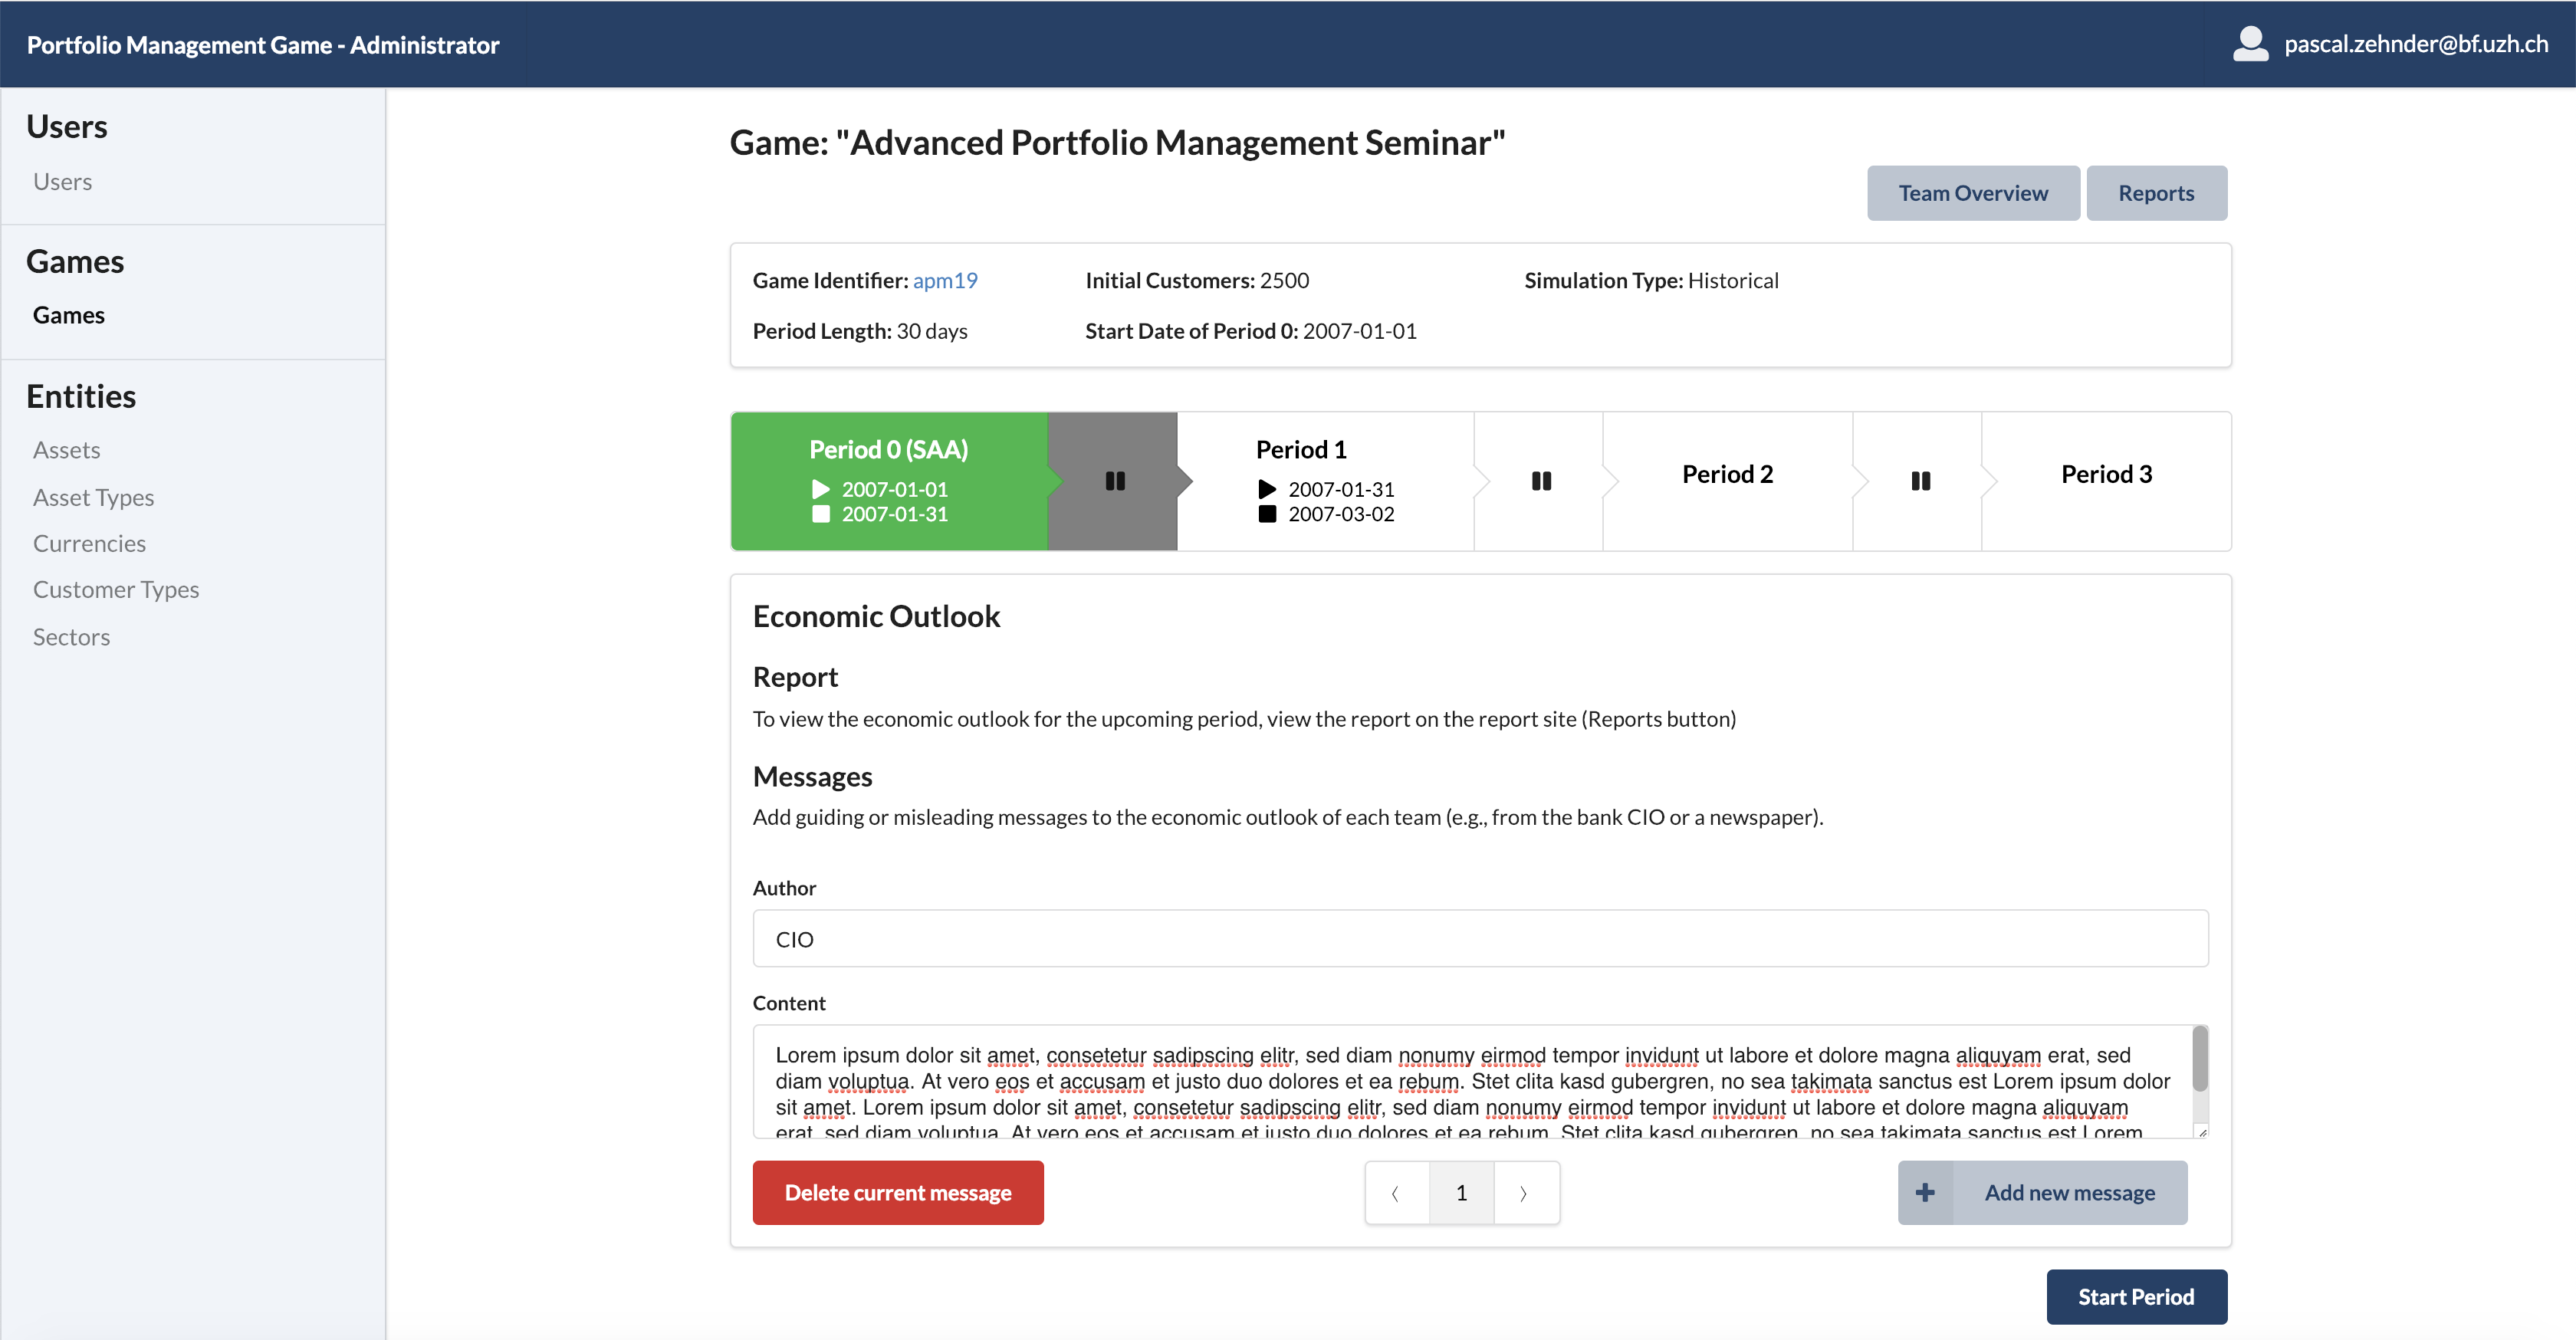
\includegraphics[scale=0.2]{img/application-overview/administrator/09_period_start.png}
  \caption{Period start}
\end{figure}

\subsubsection{Reports}
For the presentation of the teams result in between two running periods being played, a report is accessible for the administrator. A more detailed description will be in section X, as the teams access the same reports as the administrator.


\subsubsection{Entities administration}

\paragraph{Assets}
All assets are visible within this page. They can be synchronized to the current definition within the market repository. % TODO on what?
\begin{figure}[h!]
  \centering
  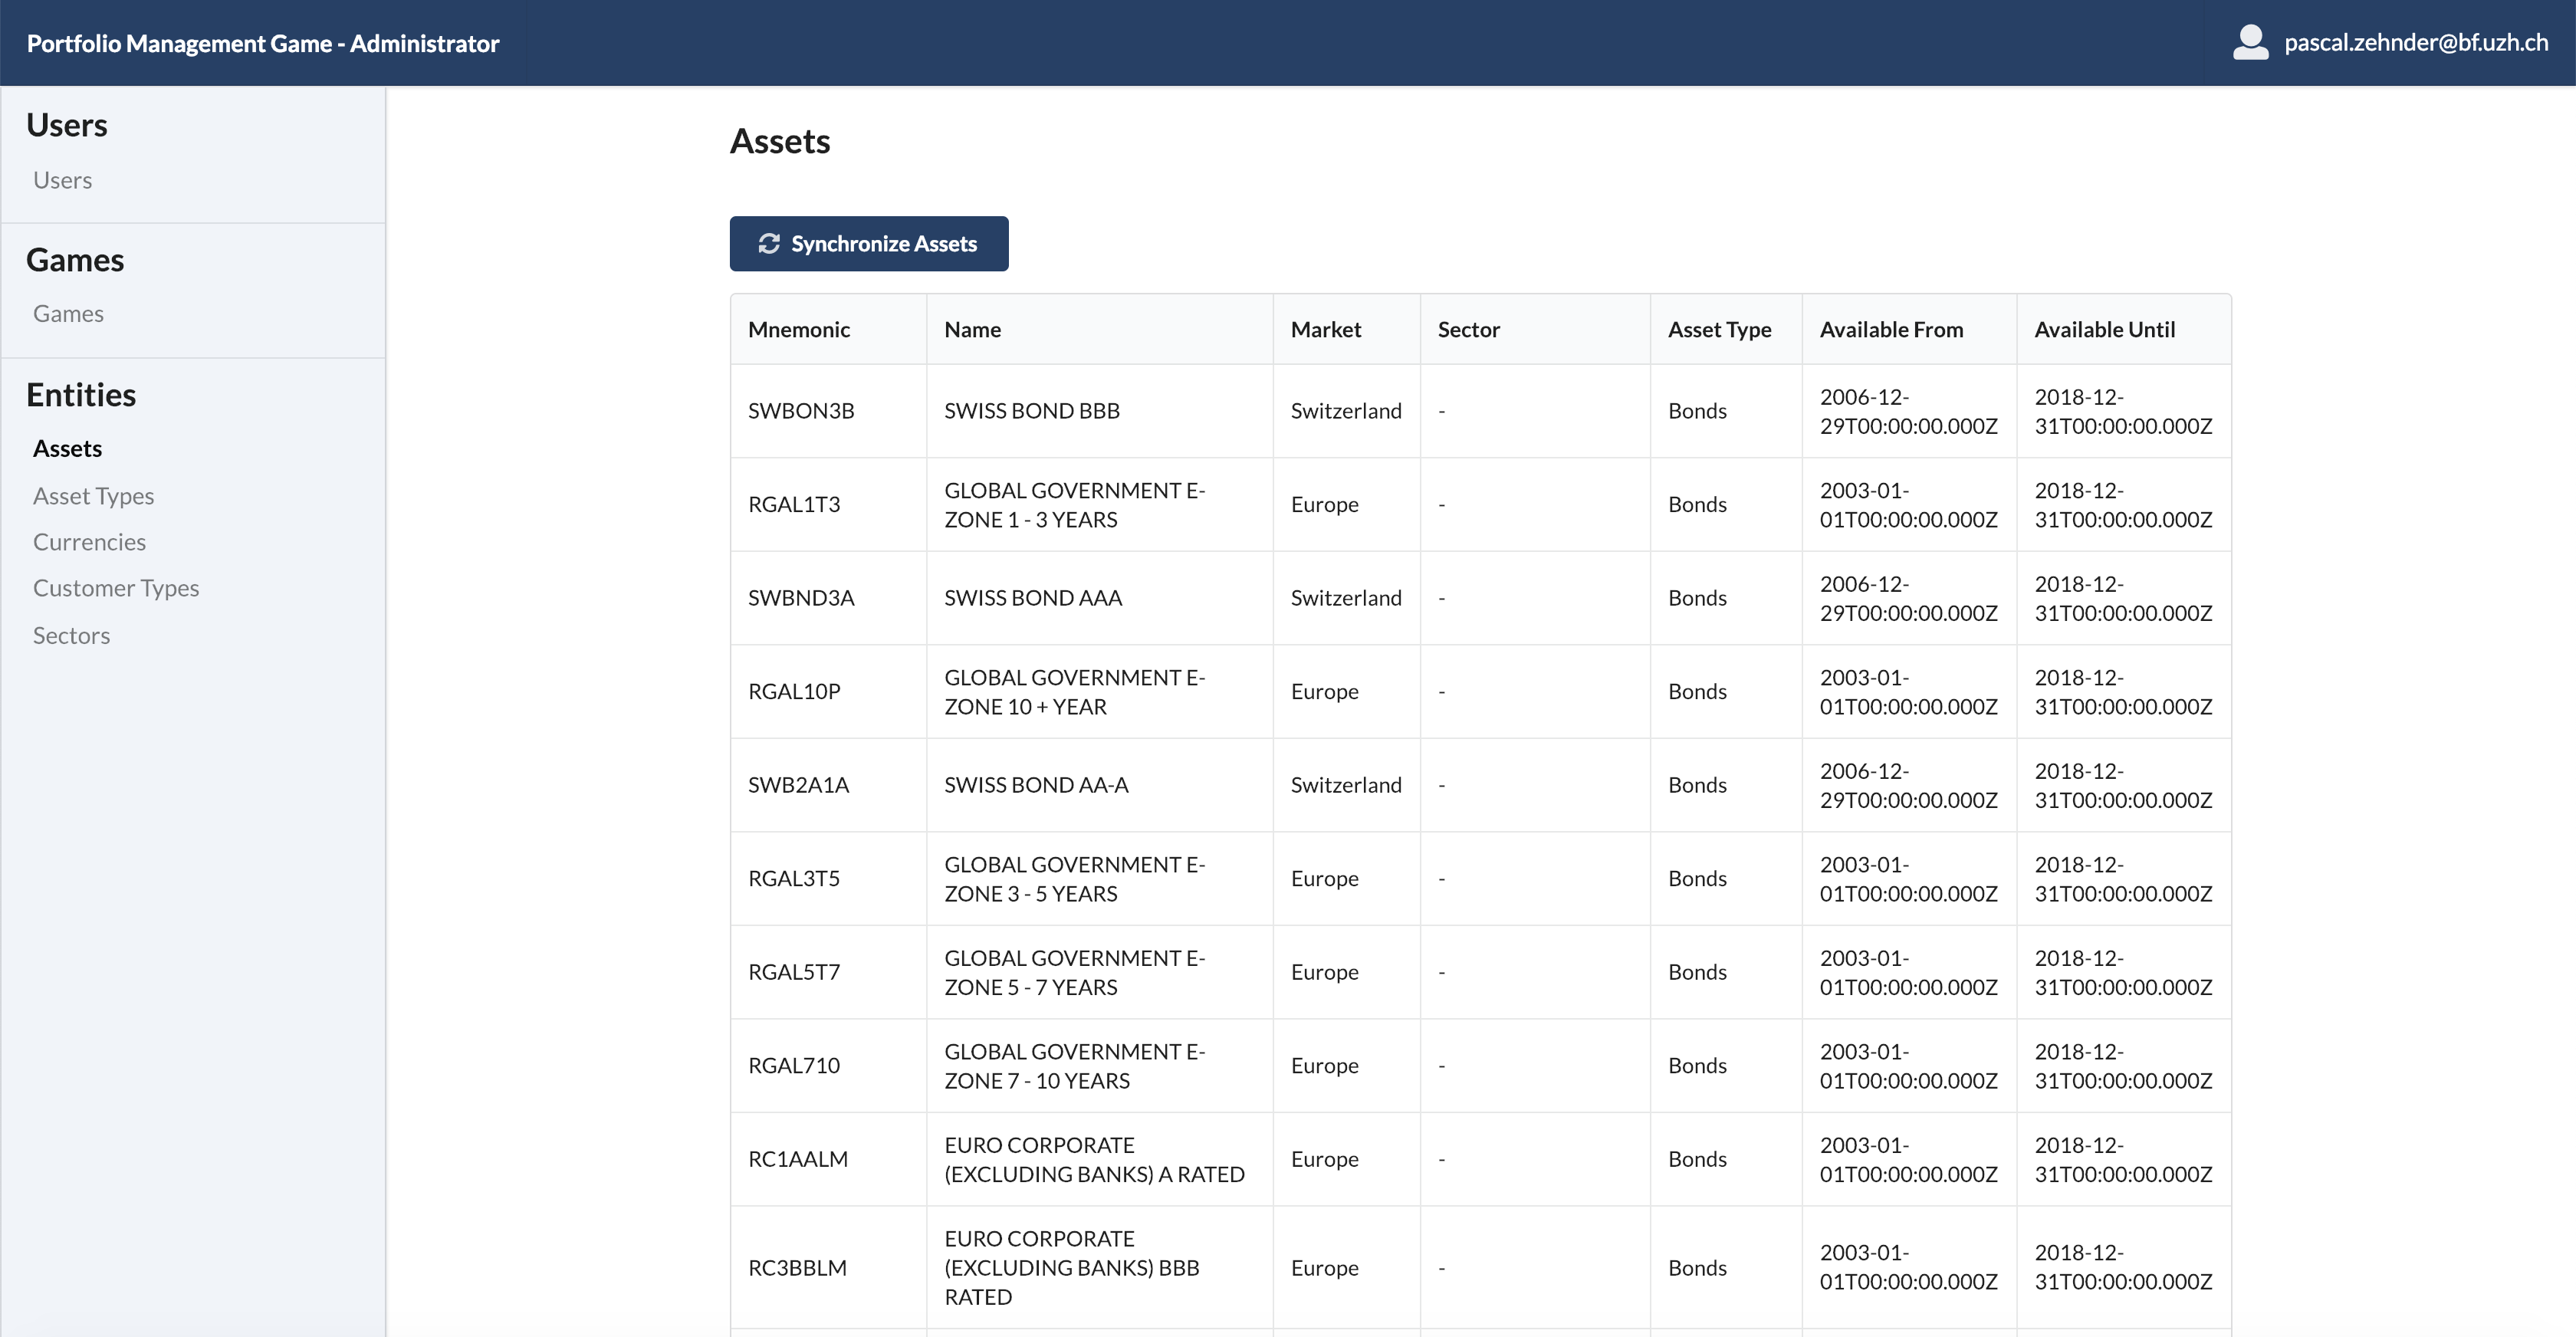
\includegraphics[scale=0.2]{img/application-overview/administrator/entities_assets.png}
  \caption{Assets administration}
\end{figure}


\paragraph{Asset Types}
A table showing all asset types which may be edited is the landing page of this entity. By editing a specified asset type the administrator can change some characteristics of its type, such as info text as shown in figure~\ref{fig:asset_types}.
\begin{figure}[h!]
  \centering
  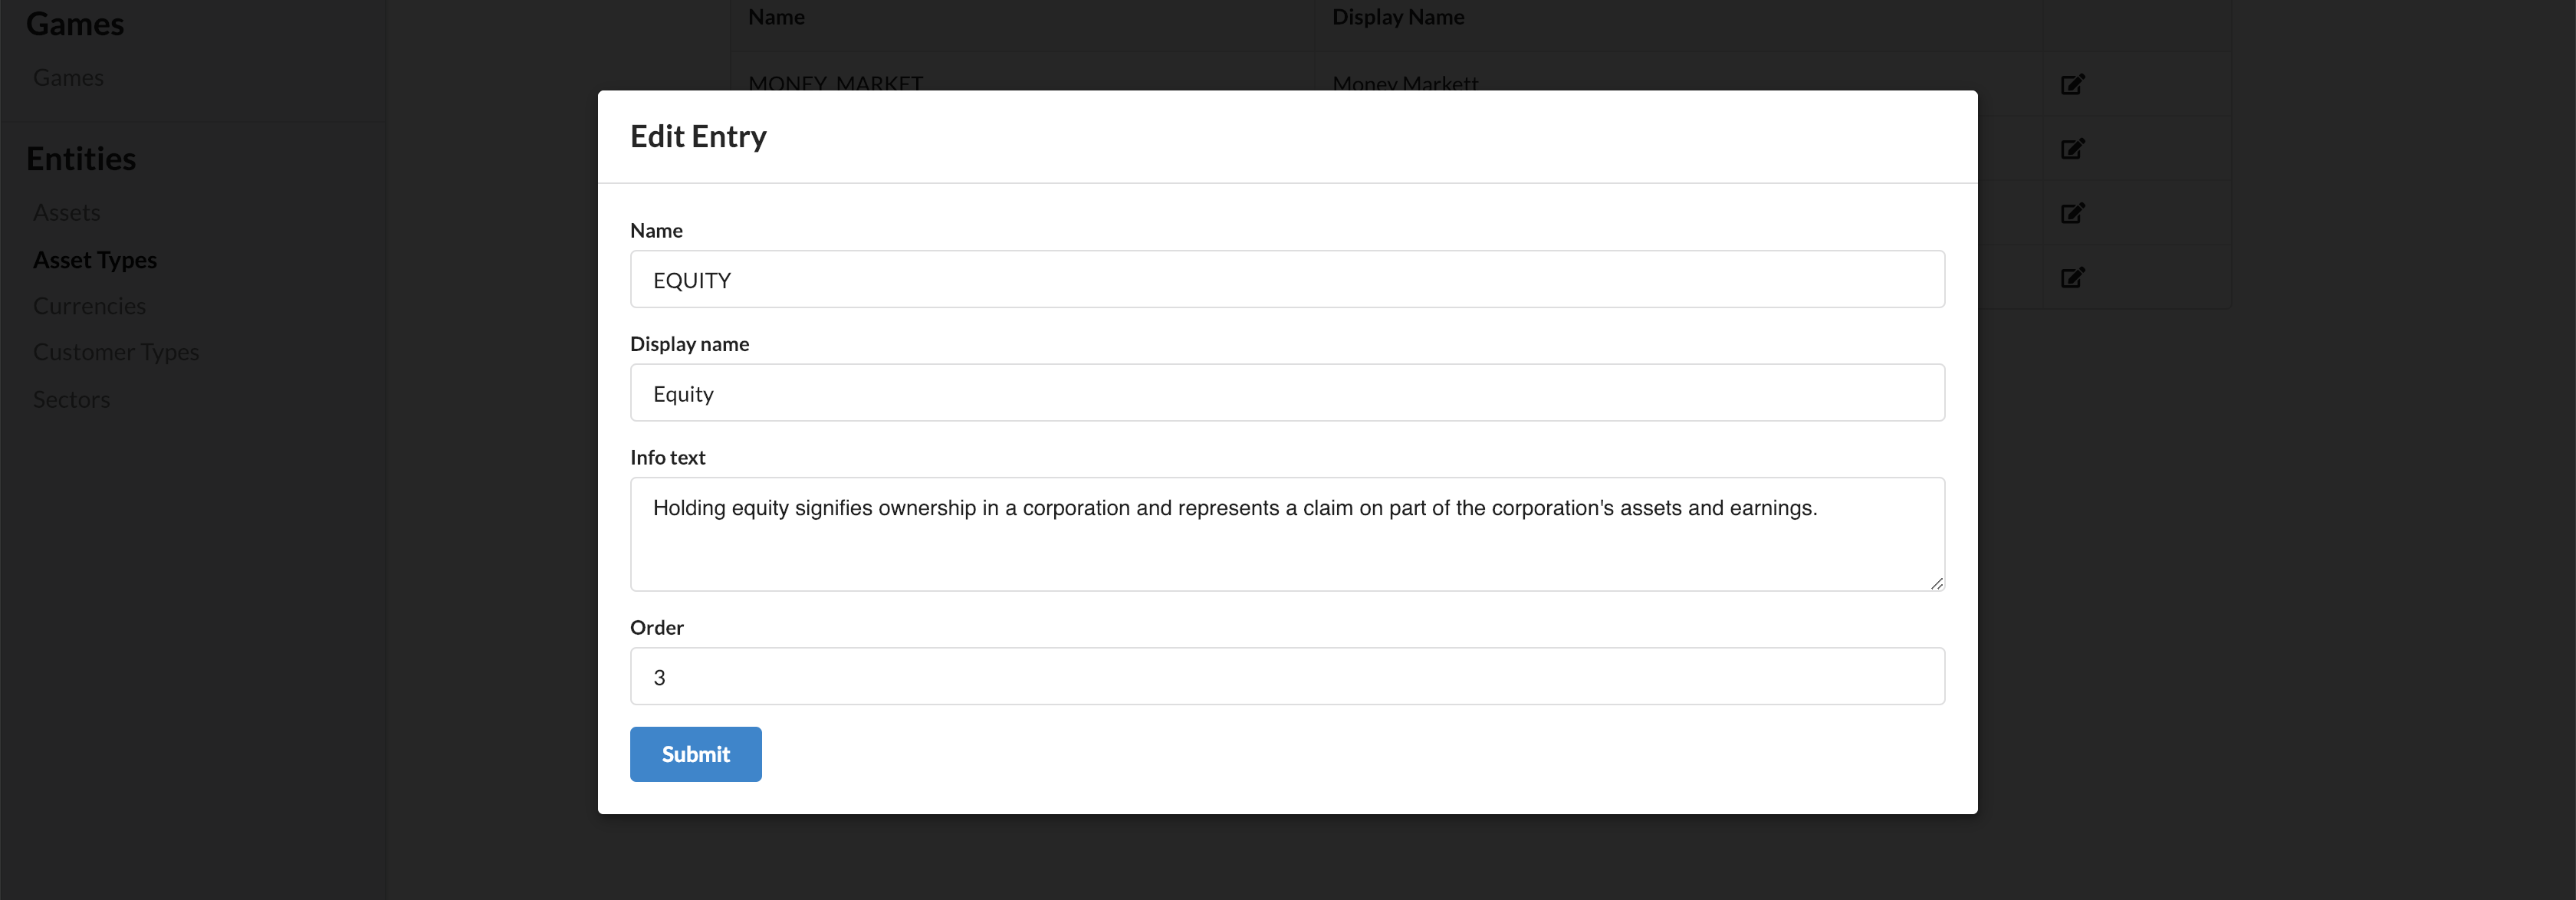
\includegraphics[scale=0.2]{img/application-overview/administrator/entities_asset_types.png}
  \caption{Asset types administration}
  \label{fig:asset_types}
\end{figure}

\paragraph{Currencies}
The currencies may be edited in the same manner as the asset types. By submitting the displaying name or symbol of the corresponding currency may be changed.

\paragraph{Customer Types}
An overview of all in the game available customer types is provided for the administrator. For each customer type, the ideal strategic asset allocation and the ranges for currencies and asset types (both dimensions) can be modified. Additionally, the info bullets and the displaying name may be modified too.
\begin{figure}[h!]
  \centering
  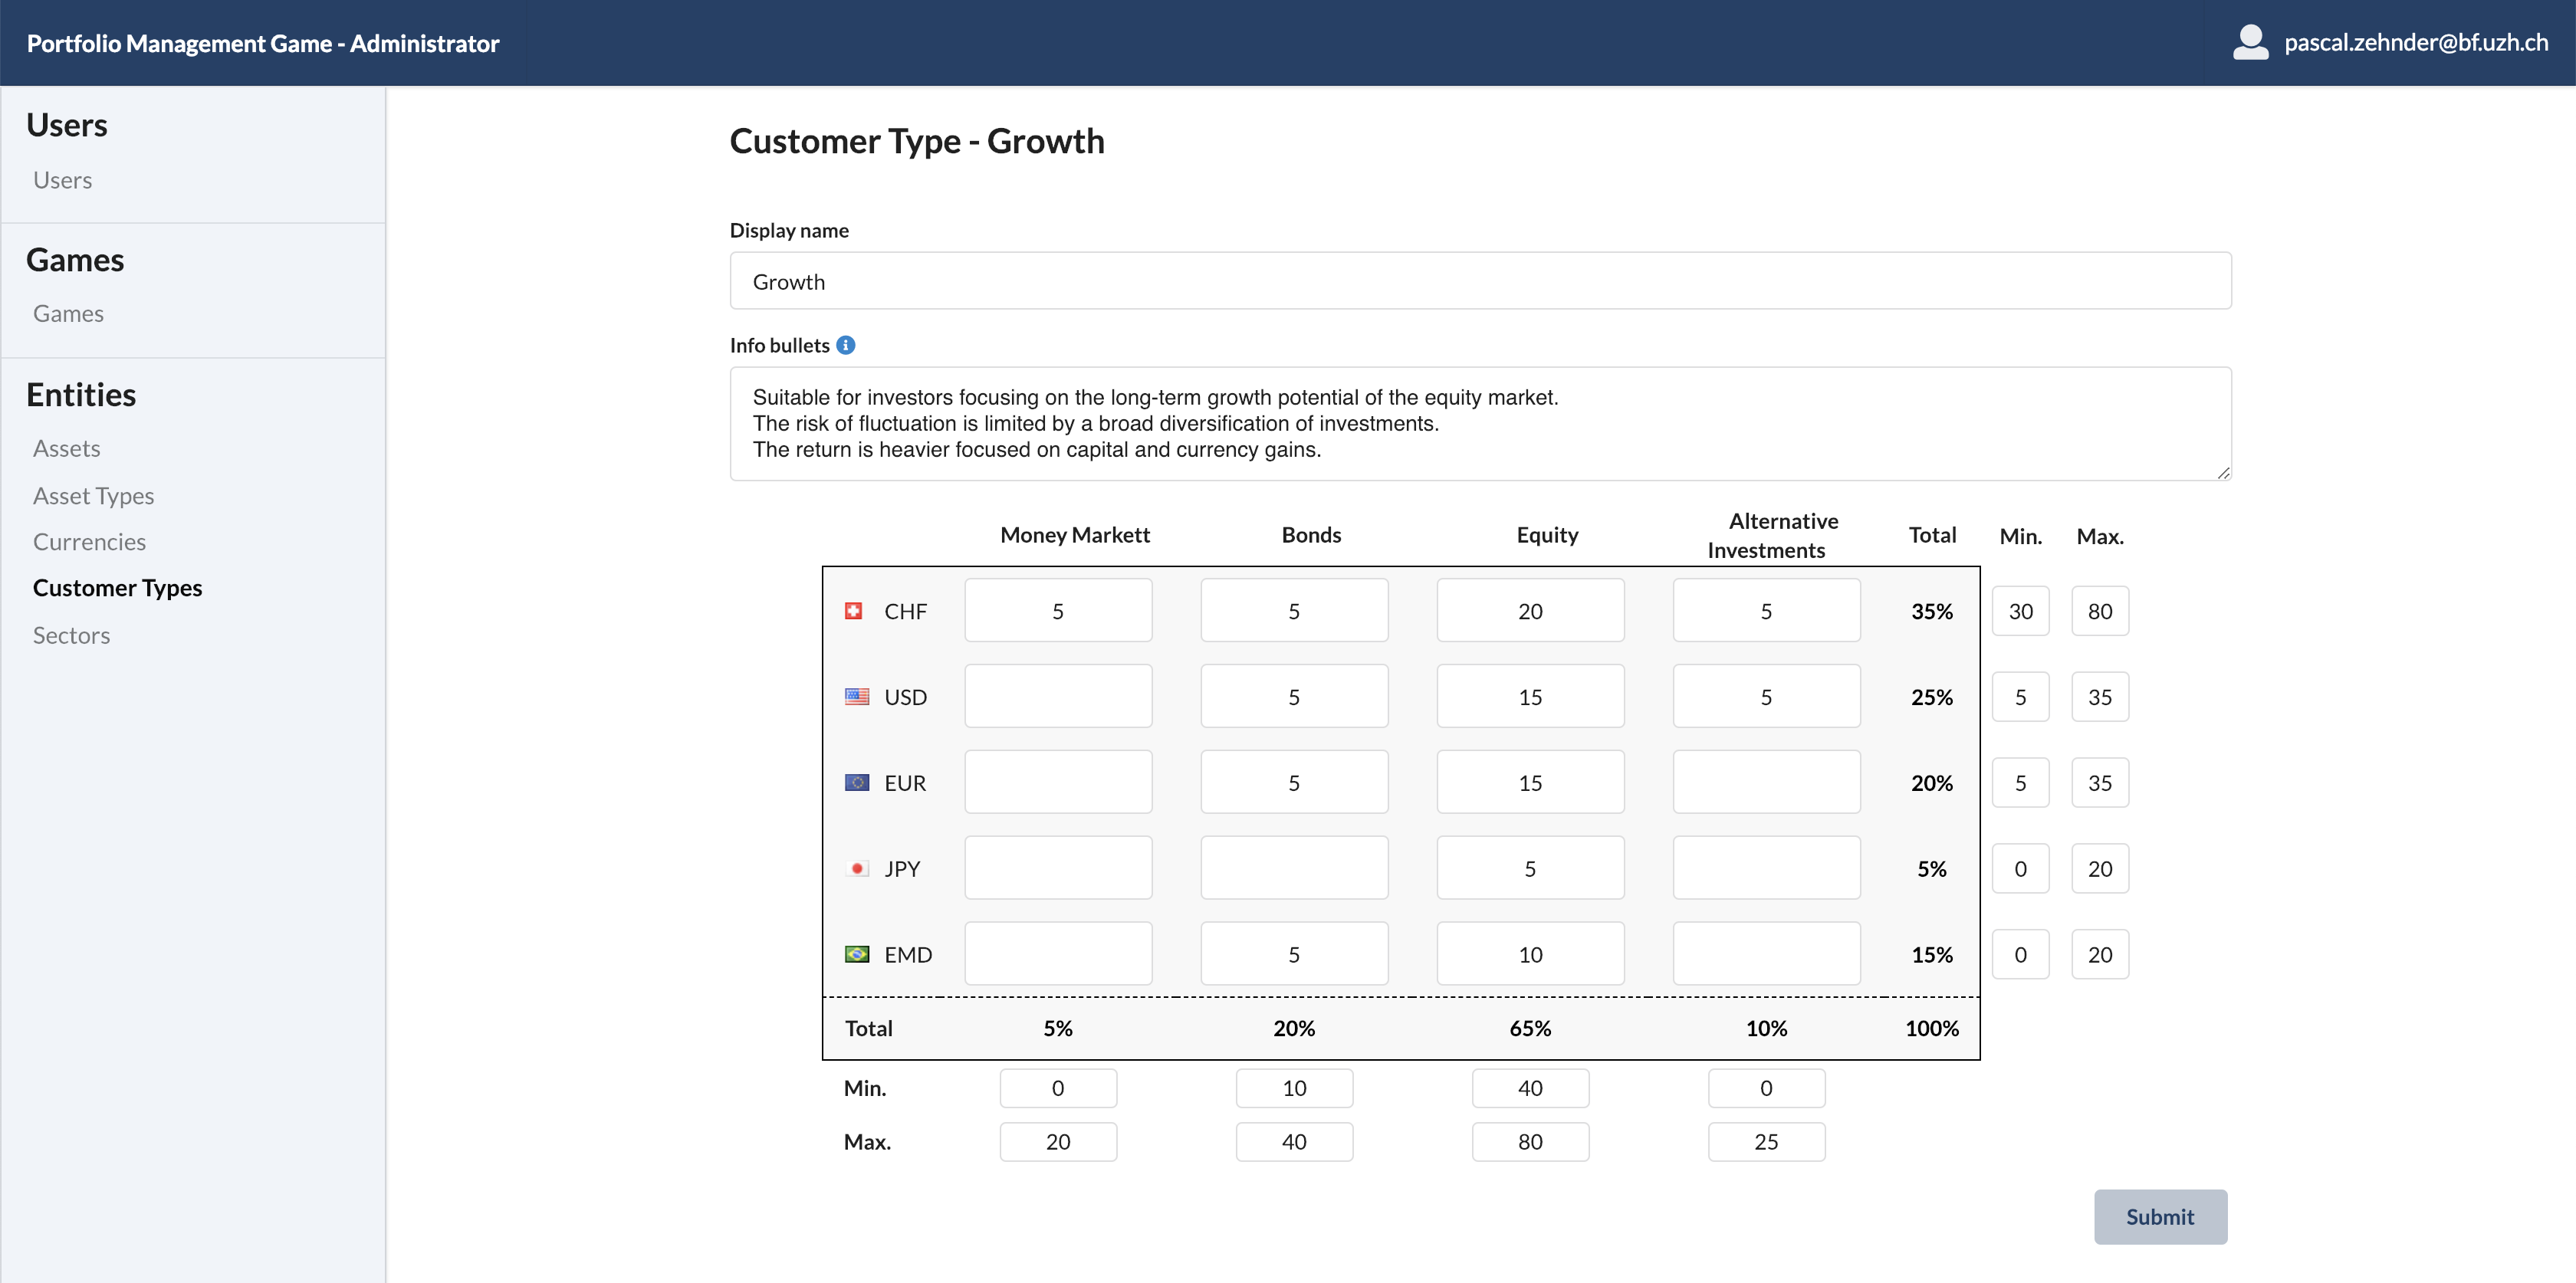
\includegraphics[scale=0.2]{img/application-overview/administrator/entities_customer_types.png}
  \caption{Customer types administration}
\end{figure}


\paragraph{Sectors}
A short overview of all sectors which are used in the asset overview.





\subsection{Team View}

\subsubsection{Login}
%\begin{center}
%  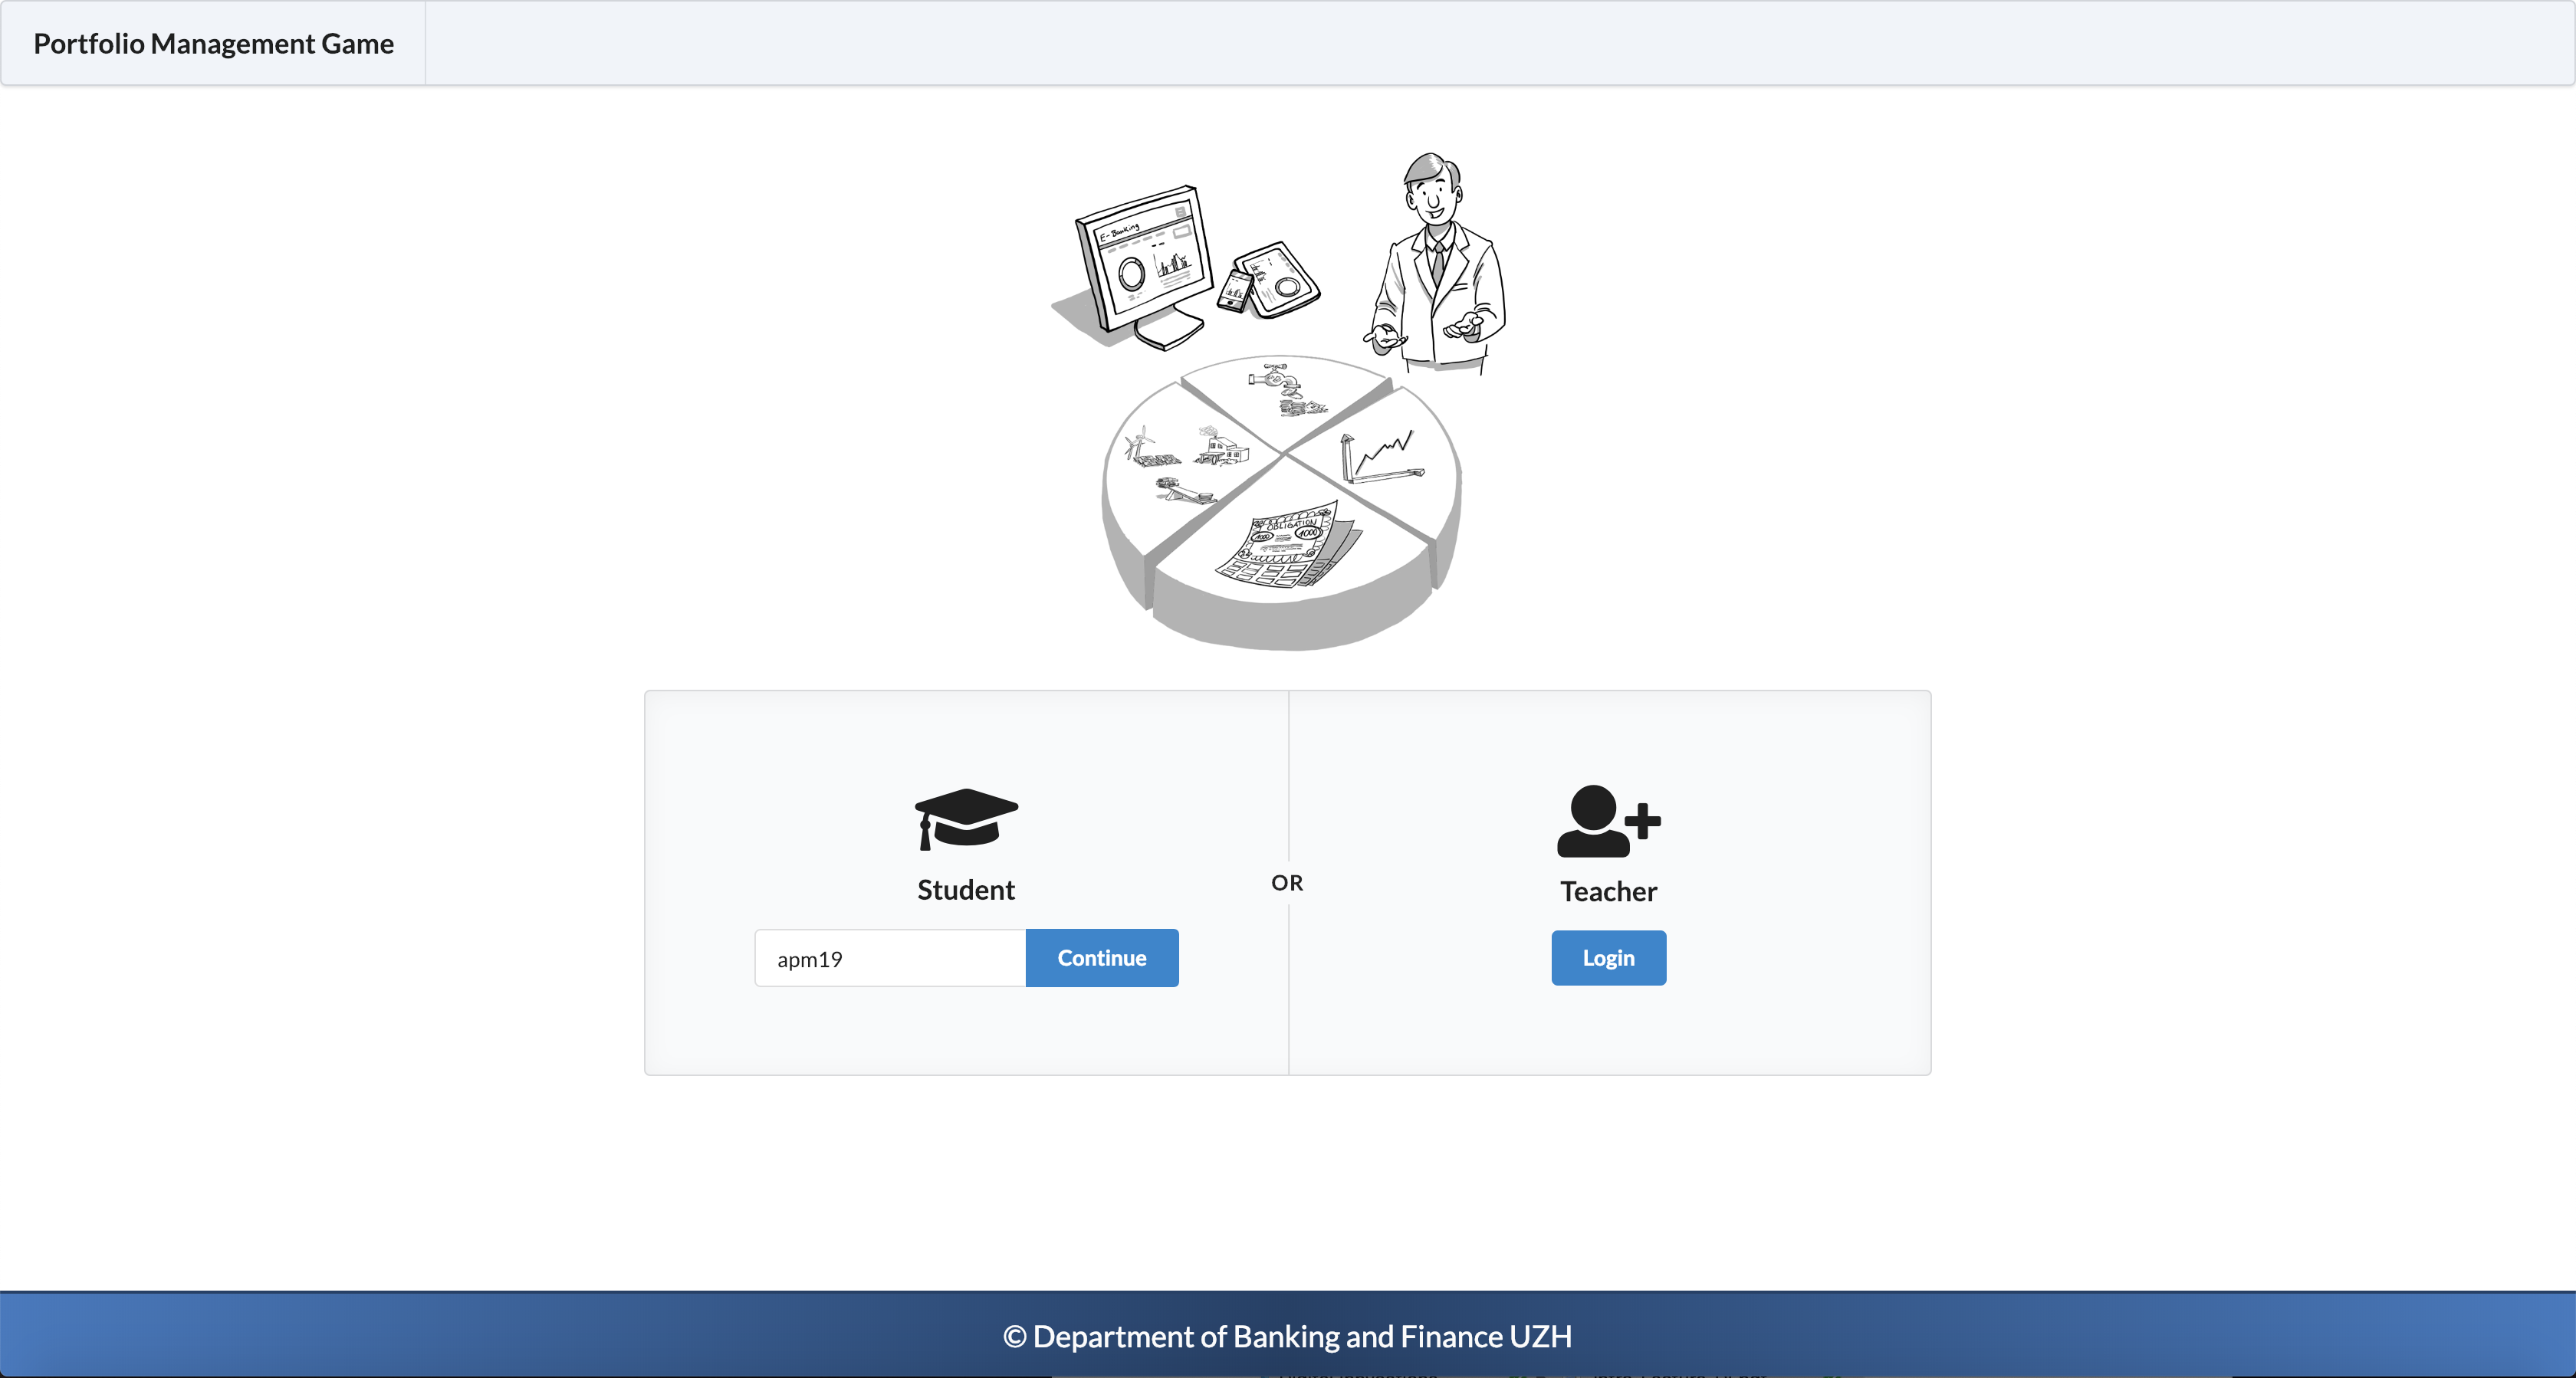
\includegraphics[scale=0.2]{img/application-overview/teams/startpage.png}
%\end{center}
By accessing the starting page, a team has to input a game short id which is provided from the administrator. Afterwards, the team has to login within a correct game identifier to participate within a game. The login credentials are accessible from the administrator screen fro each team (Paragraph~\ref{subparagraph:team_overview}).
\begin{figure}[h!]
  \centering
  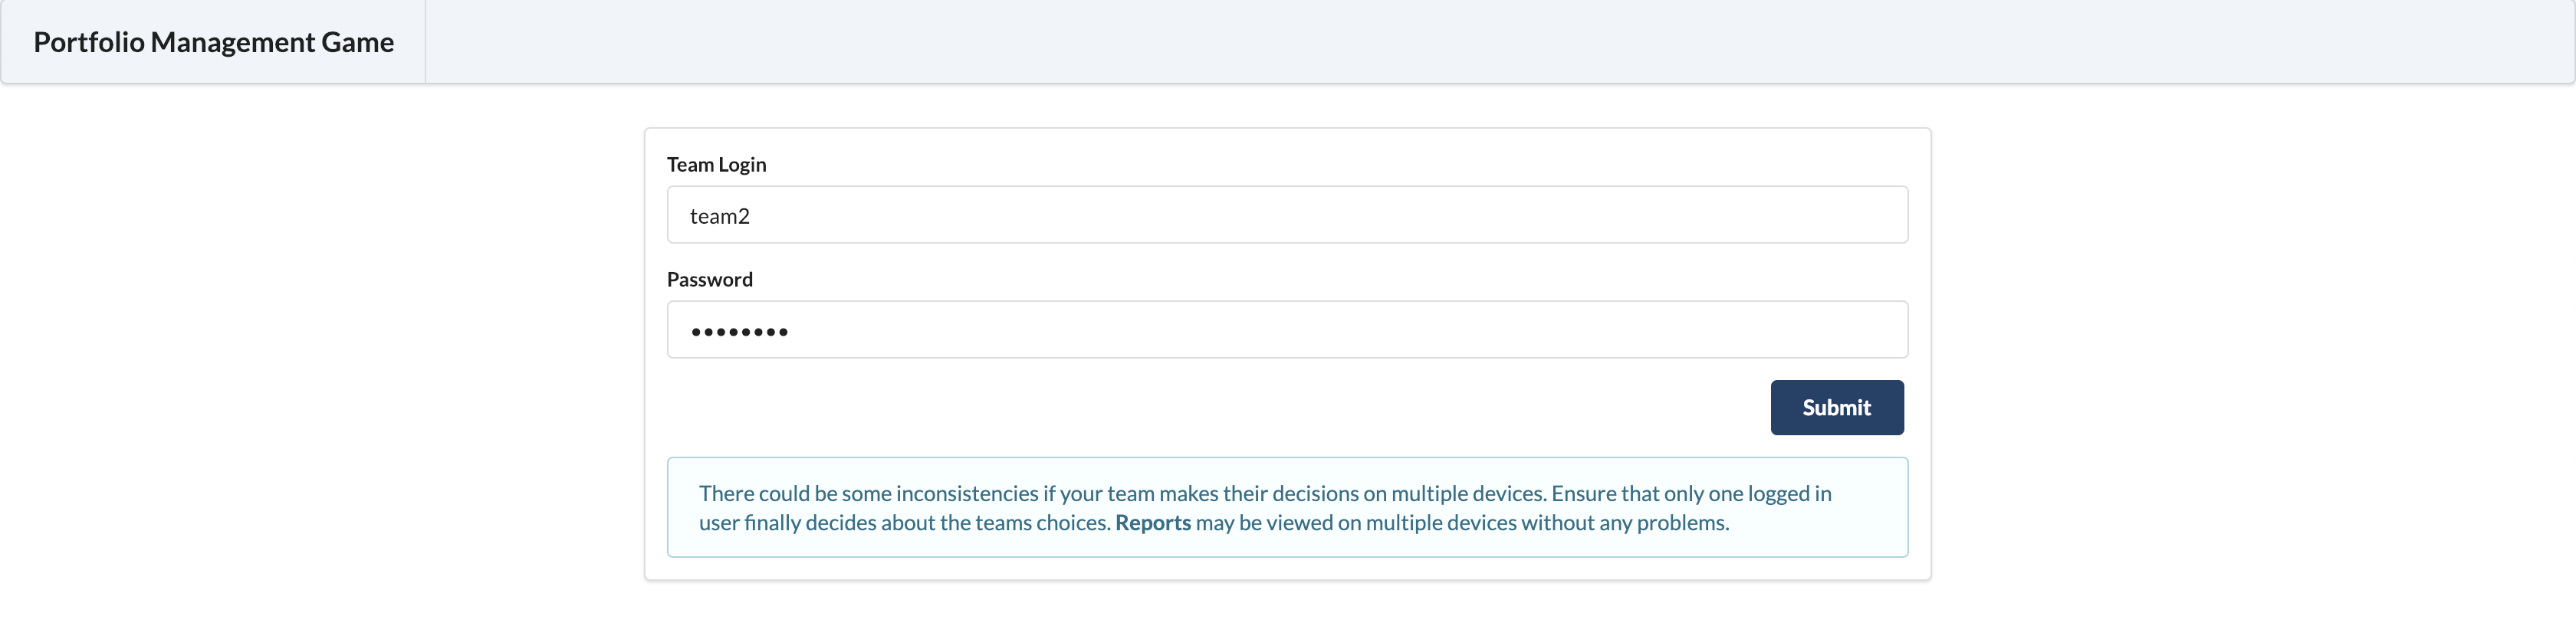
\includegraphics[scale=0.2]{img/application-overview/teams/01_login.png}
  \caption{Team login}
\end{figure}

\subsubsection{Period 0 decisions}
In period 0 which represents phase 1 of the game, the teams define their SAA for all customer types which are enabled by the administrator of the specific game. The teams need to fulfill the ranges for all dimensions to submit their decisions. Supportive graphs in form of pie charts help the teams to decide about the share of the two dimensions. Additionally, the players can name their team on the top left corner of the screen.
\begin{figure}[h!]
  \centering
  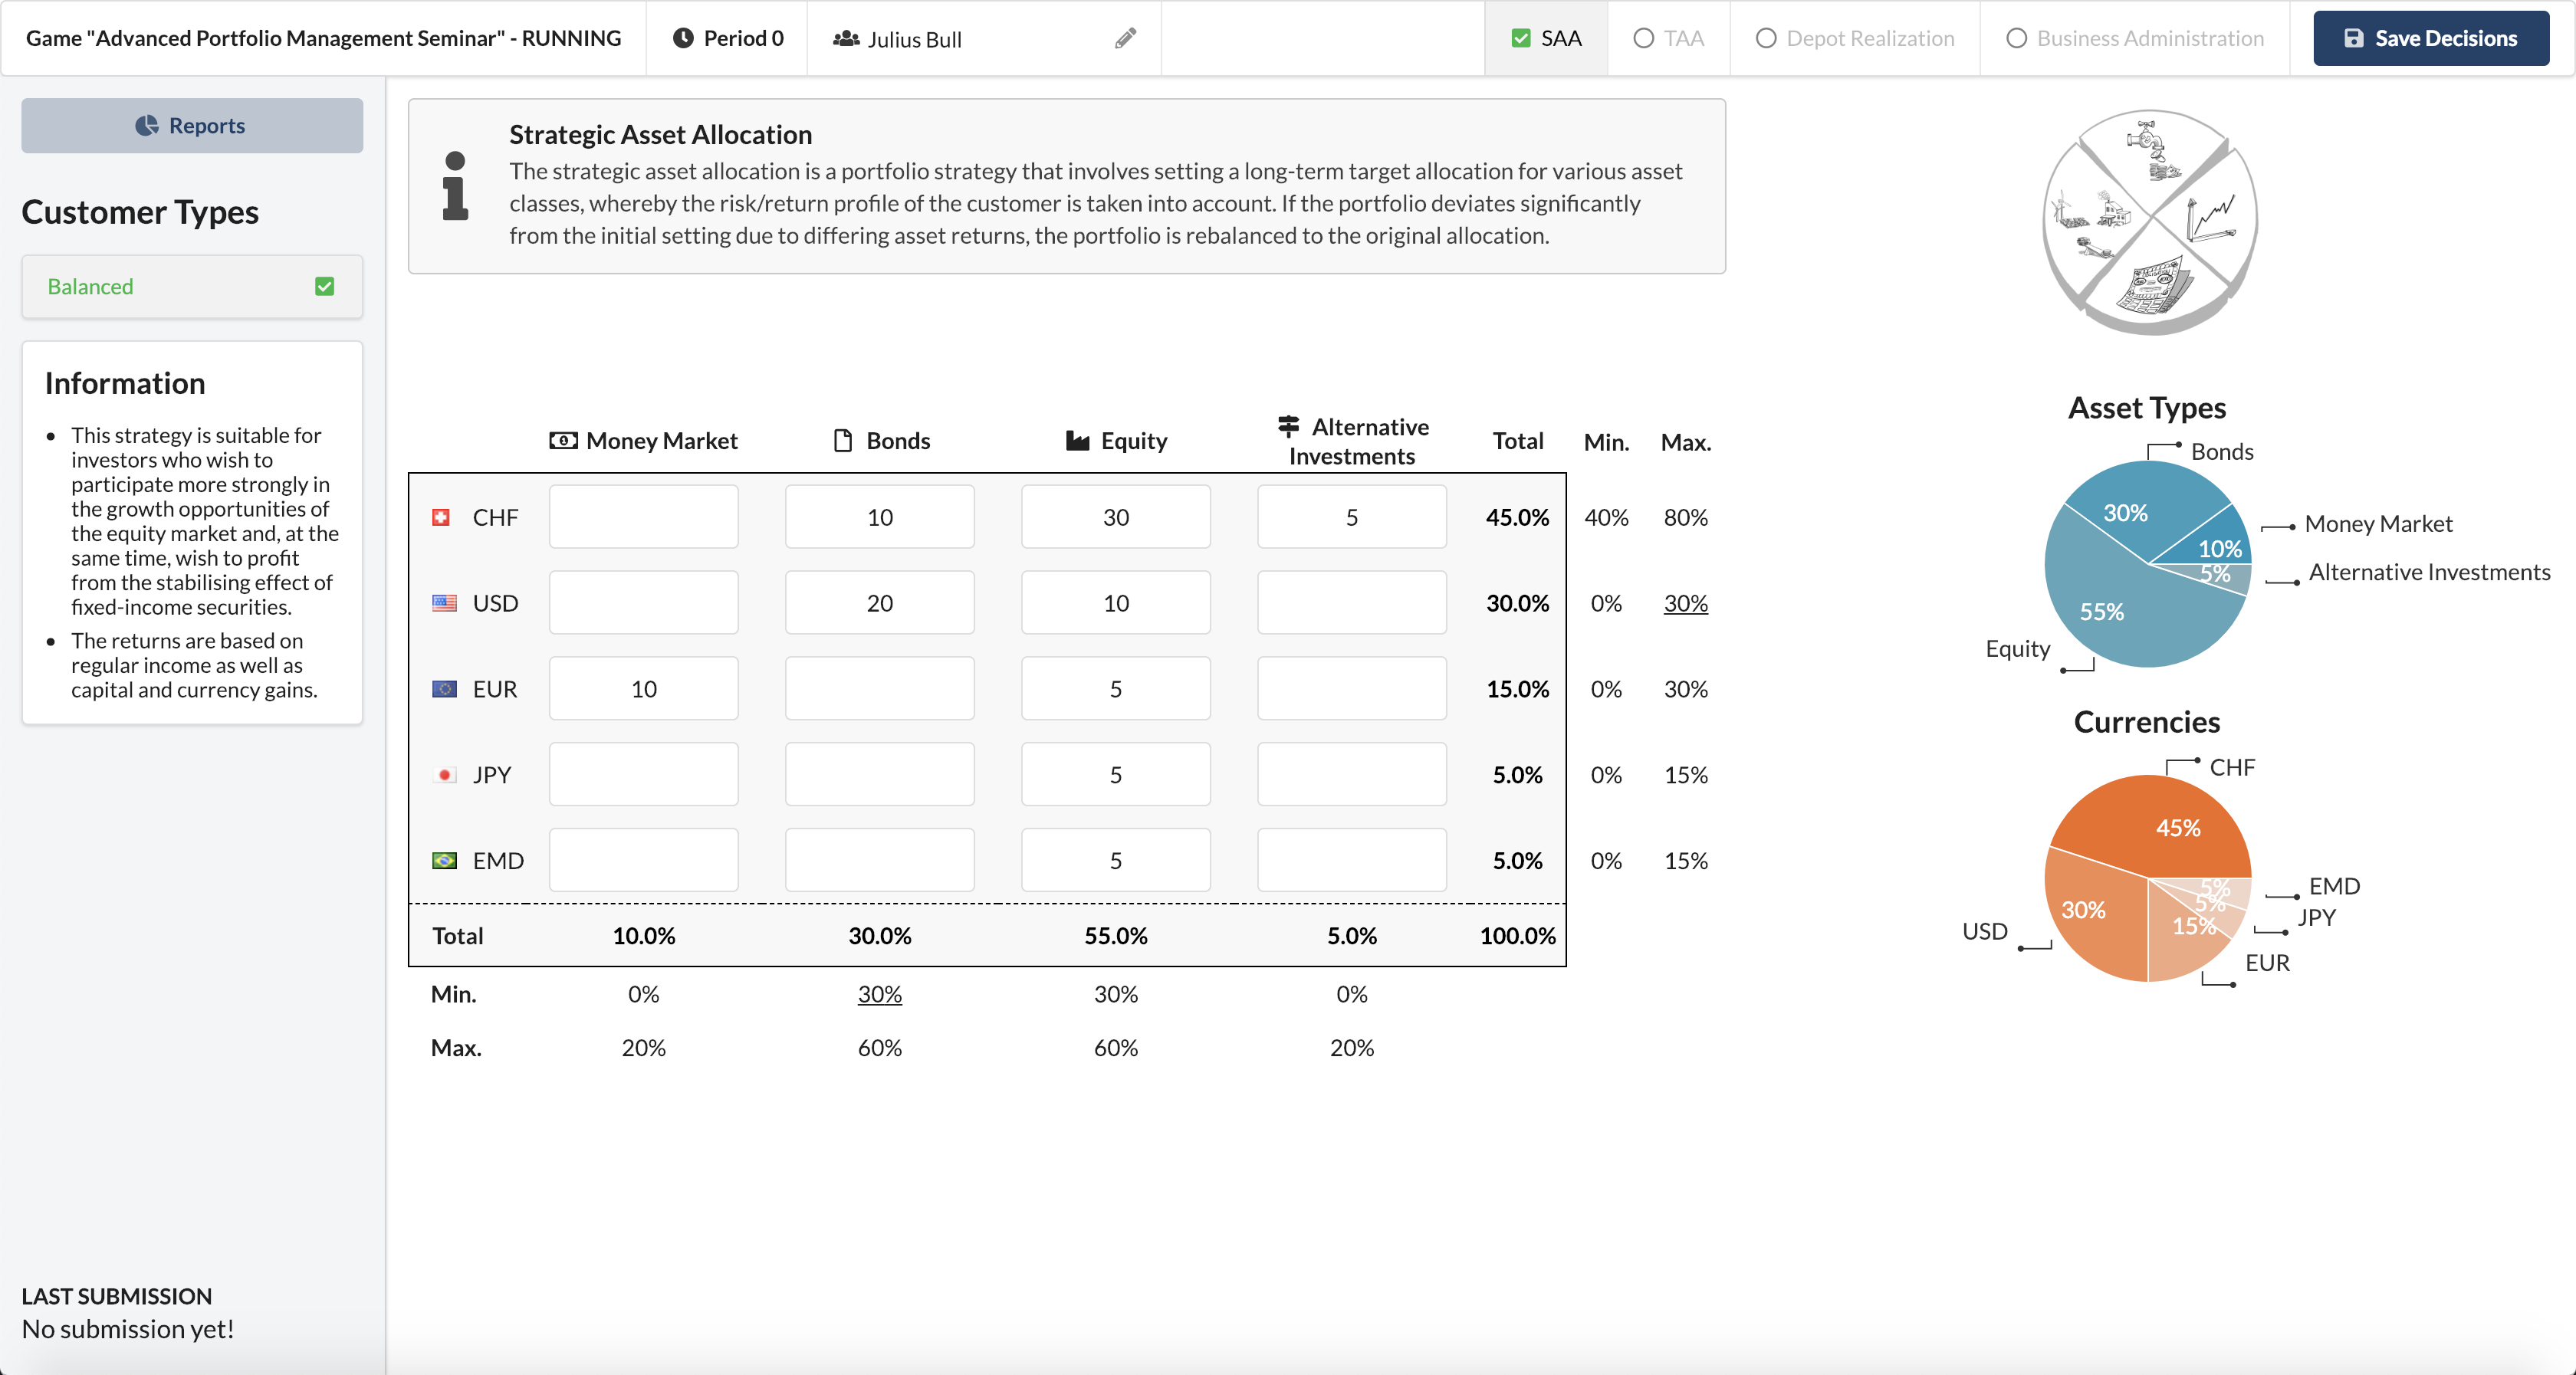
\includegraphics[scale=0.2]{img/application-overview/teams/02_period_zero_decisions.png}
  \caption{Period zero decisions}
\end{figure}

\subsubsection{Other periods decisions}
Starting from period 1, a team has to complete multiple decisions separated into four pages. Strategic asset allocation is fixed and not editable for a customer type which was defined at the beginning of the game. When the administrator defines a new customer type for an upcoming period, the teams have to allocate an SAA for the new customer type.\\

For each step within this process, a progress state helps the teams to understand the state of each step. For saving their decisions, all four steps have to be completed. In the bottom left corner, the submission state may be seen.

\paragraph{TAA}
For the tactical asset allocation, the teams can deviate from the SAA due to changes in the overall market. Equal to the strategic asset allocation screen the teams change the input within the table and get illustrative support with two graphs, displaying the allocations for both dimensions of the table. Initially, the inputs from the strategic asset allocation are loaded, whereas the students can adjust them to market changes. Arrows within the total summation of each asset type or currency show the status of being within the range.
\begin{figure}[h!]
  \centering
  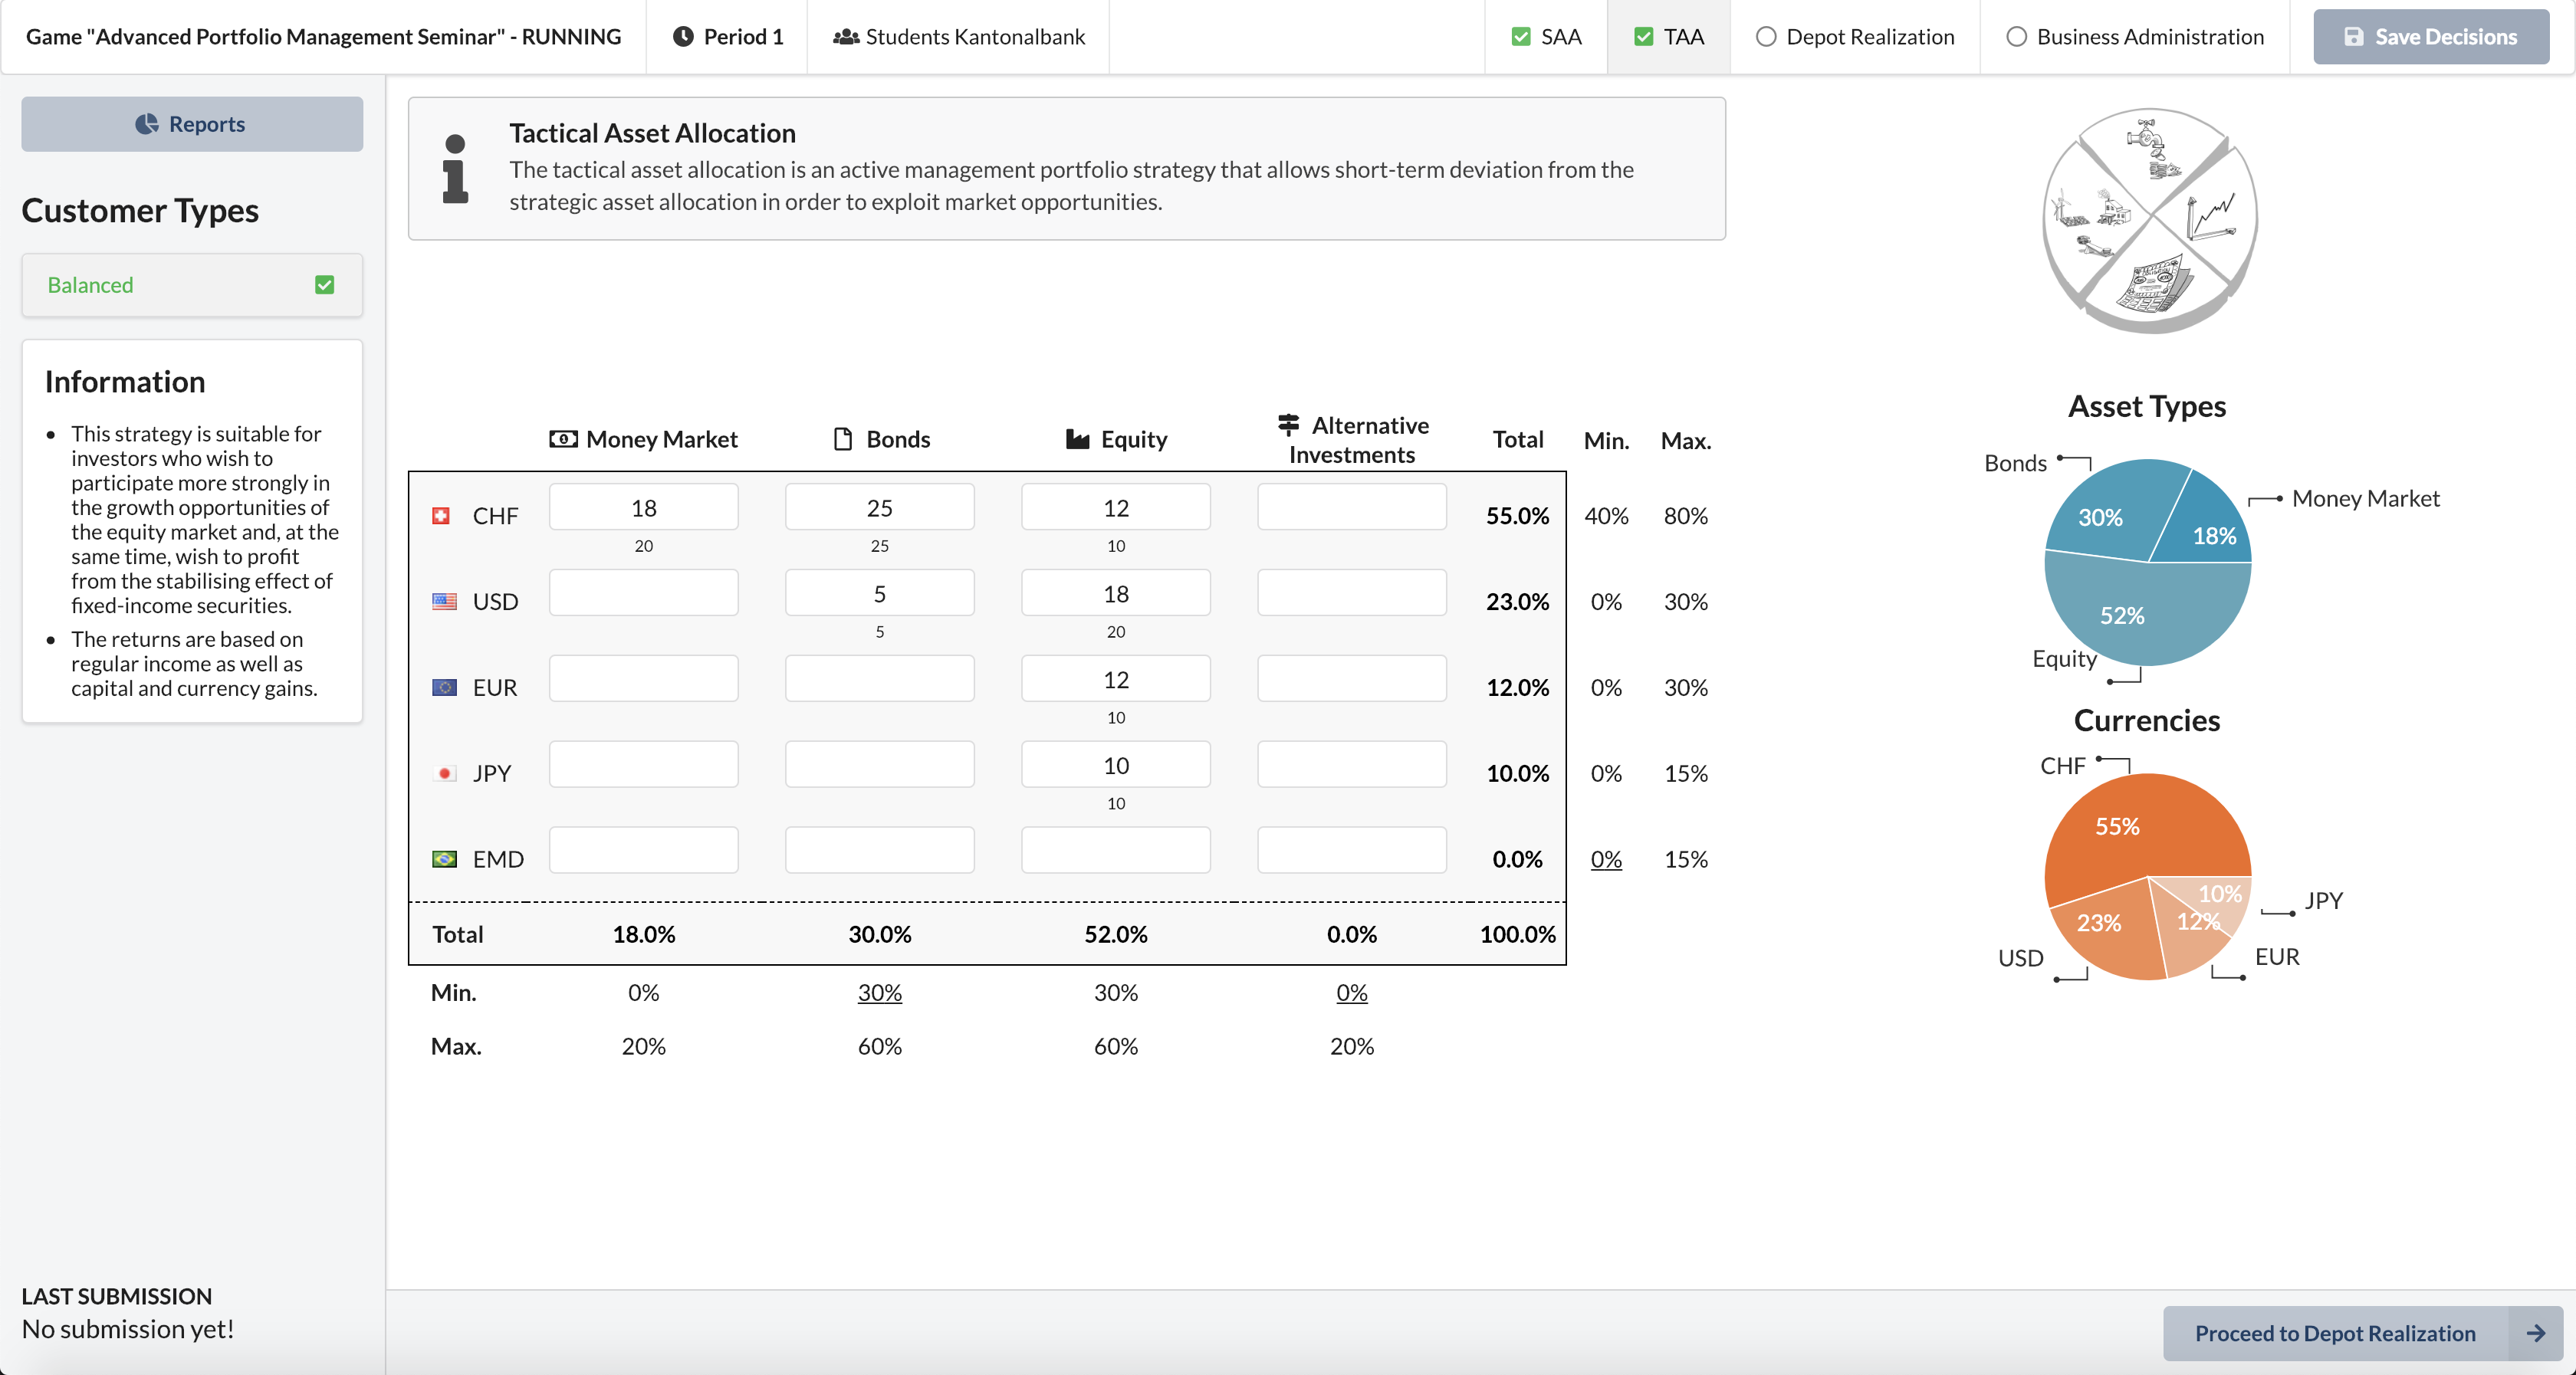
\includegraphics[scale=0.2]{img/application-overview/teams/04_taa.png}
  \caption{Tactical asset allocation}
\end{figure}

\paragraph{Depot Realization}
Based on SAA and TAA the teams finally have to allocate on specific assets. By having a bar chart on the top of the screen, students have an overview of their SAA and TAA decisions of the current active customer type. A target for the students is to allocate assets such that the yellow bar aligns with TAA for each asset type/currency combination. On the top right corner, a short summary of the most important key numbers for the allocations is present.
% TODO table description with filters etc.
This process has to be repeated for each customer type defined by navigating on the left menu. Equal to the SAA and TAA screen, the progress of the customer types is highlighted with checkmarks and corresponding colors.

\begin{figure}[h!]
  \centering
  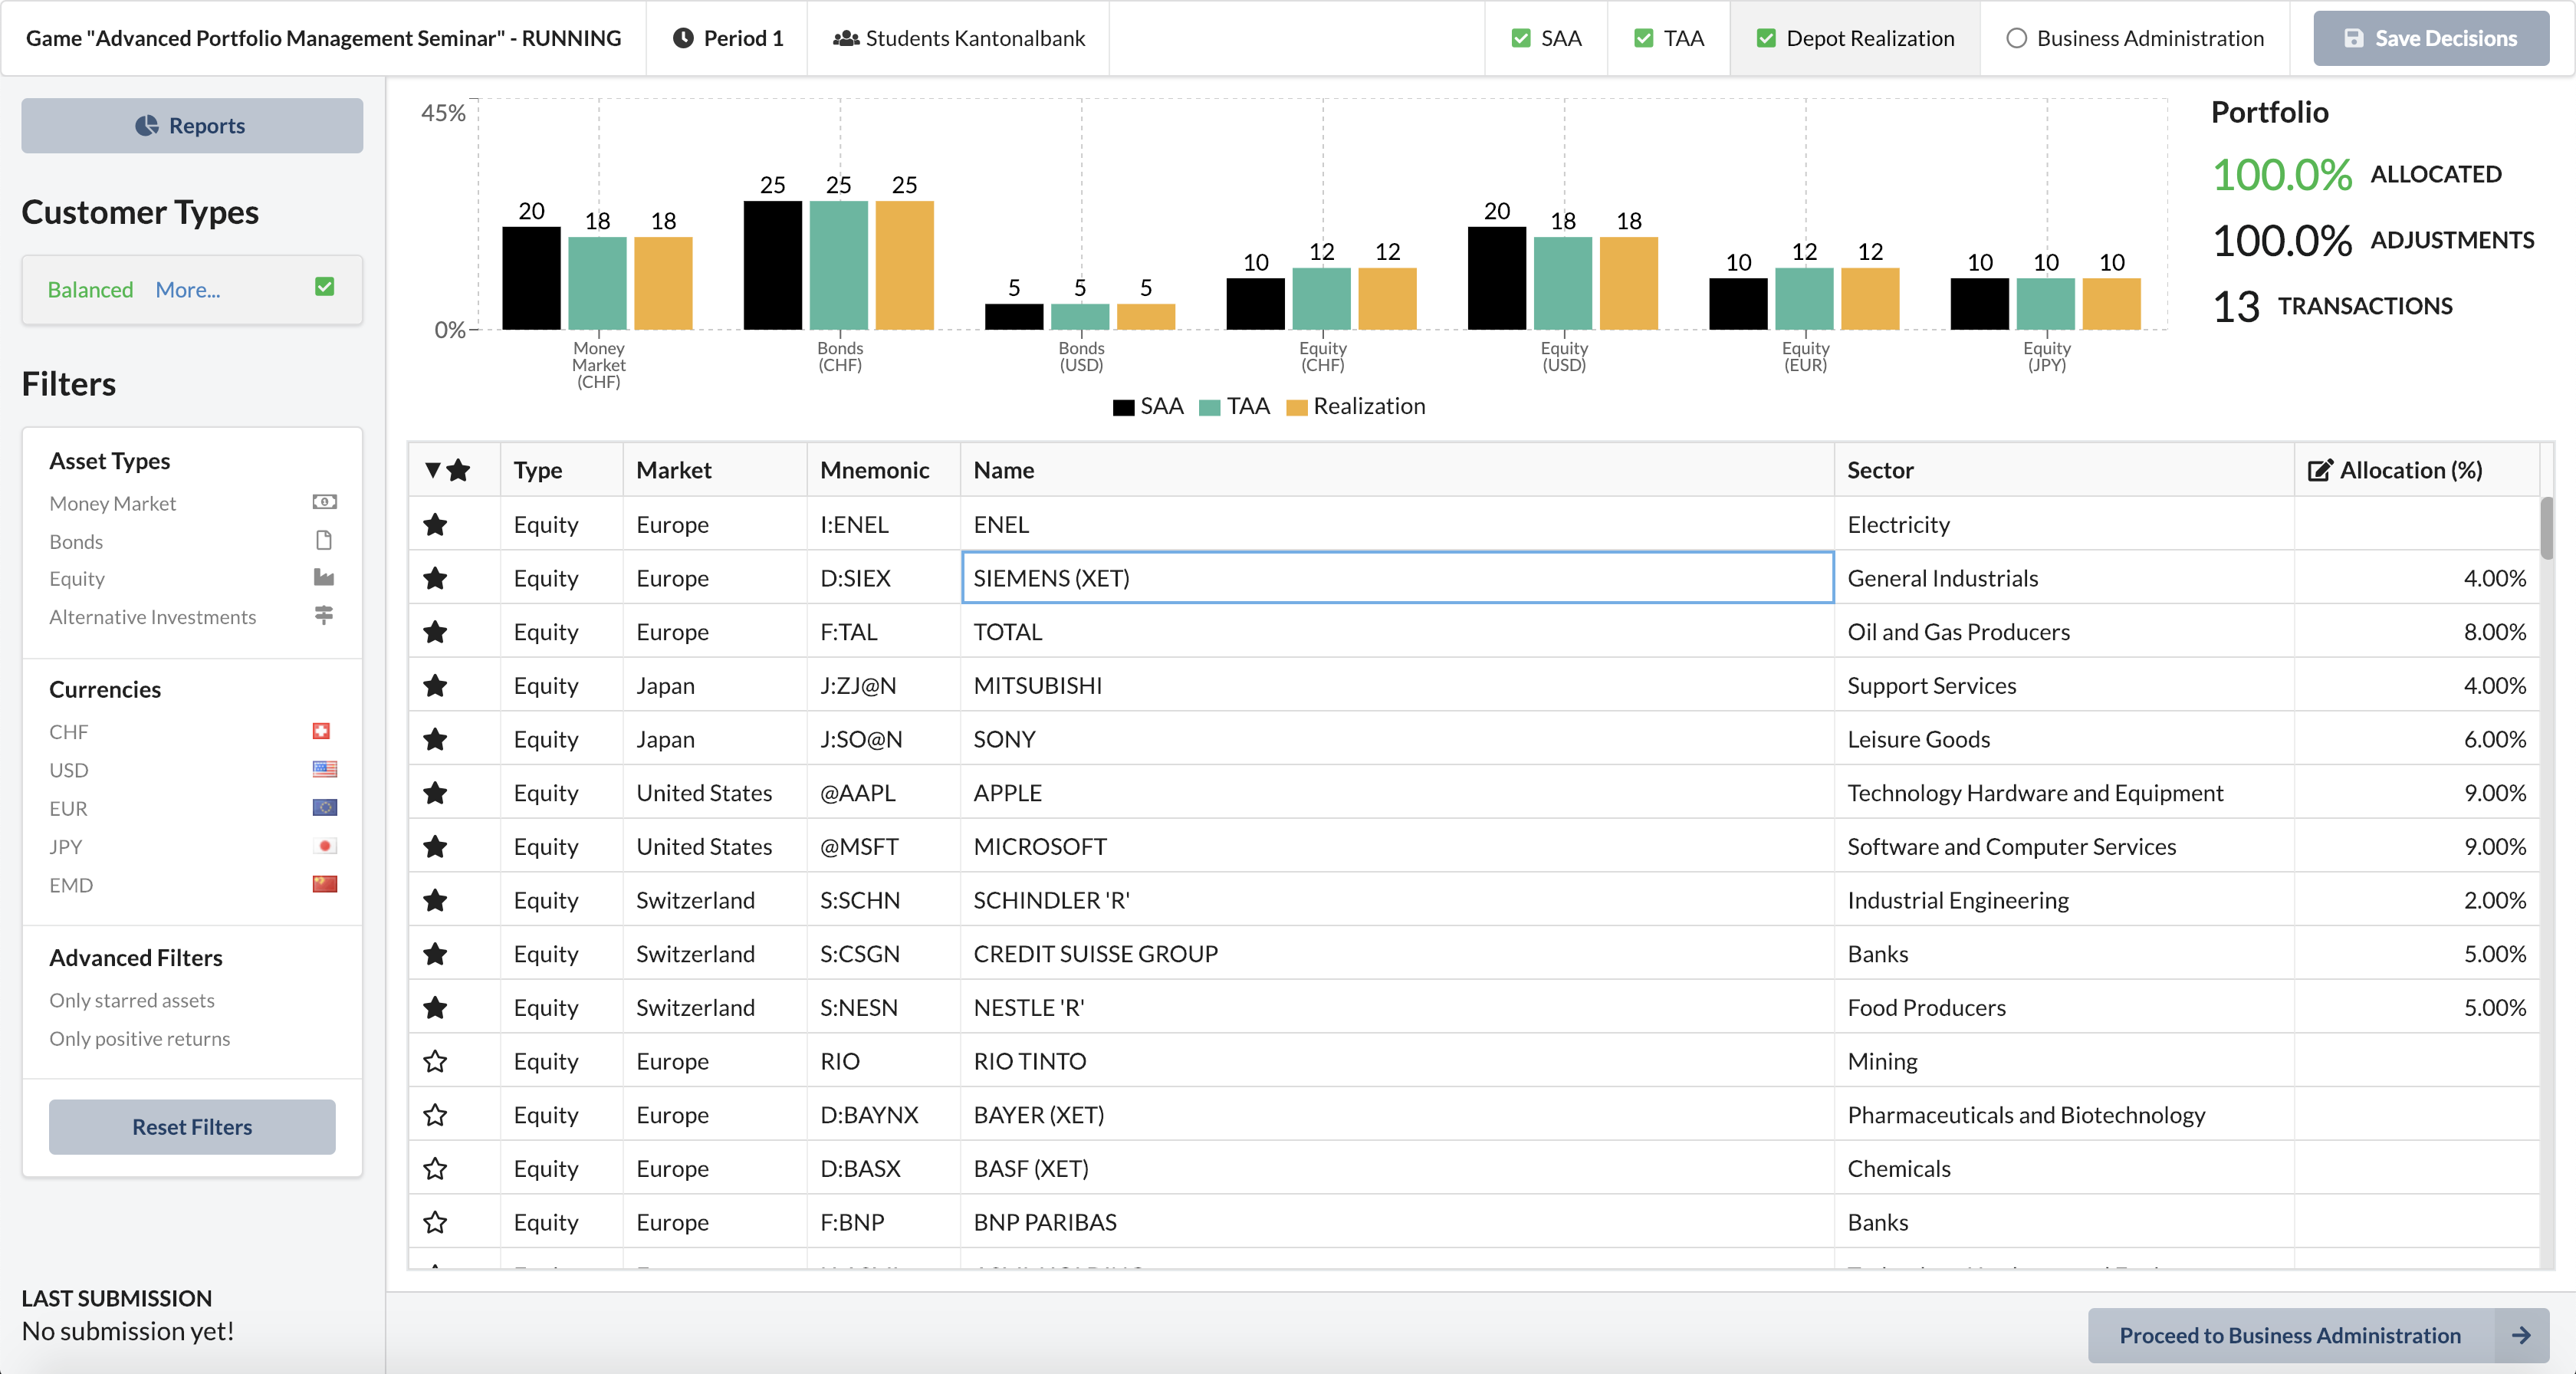
\includegraphics[scale=0.2]{img/application-overview/teams/05_depot_realization.png}
  \caption{Depot realization}
\end{figure}

\paragraph{Business Administration}
Business administration operates as the final decisions for a period. On the left side of the screen teams input numbers for four different categories: Conditions \& Fees, Human resources, logistics, and profit distribution. For each input field, the initial value (in period 1) or the previous period value (for all other periods) is displayed next to the input field.\\

On the right side, the balance sheet from the previous period is visualized to inform teams about their business results. Further key information is displayed on top of the balance sheet.
\begin{figure}[h!]
  \centering
  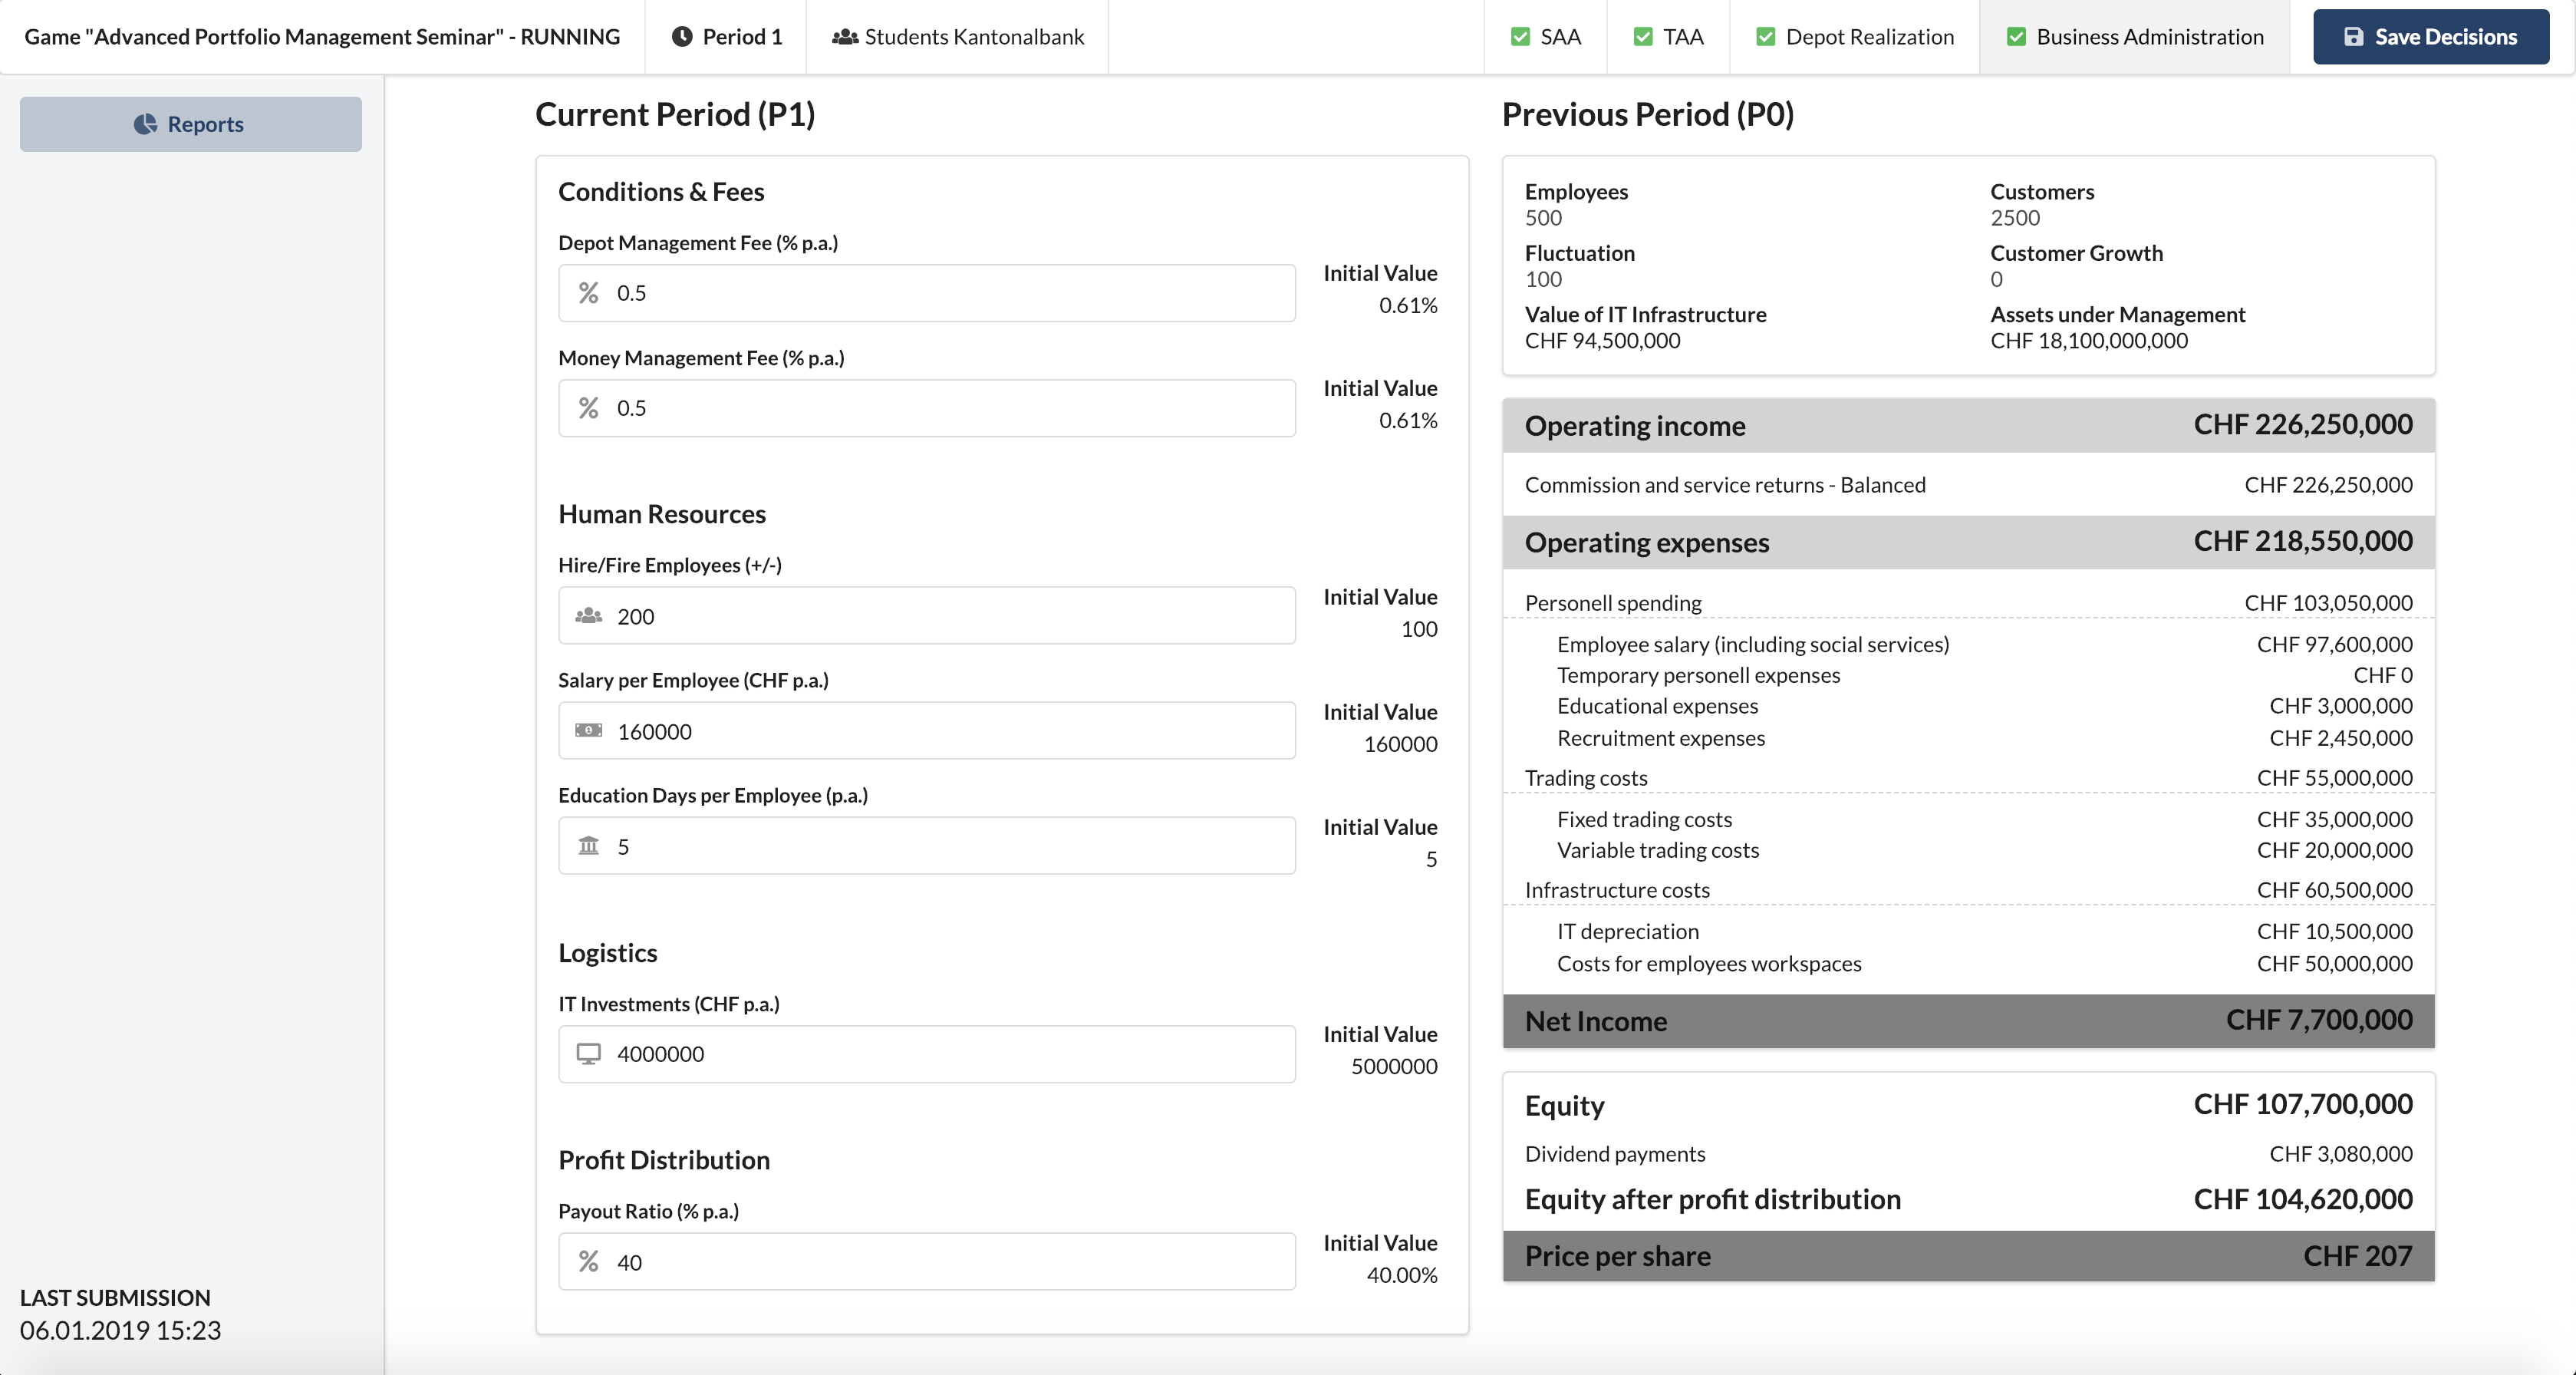
\includegraphics[scale=0.2]{img/application-overview/teams/06_business.png}
  \caption{Business administration}
\end{figure}

\subsection{Reports}
Reports are available for both administrators of a game and teams. They explain the results of the different periods of each team and compare them to the results of the other teams. As there are many graphs available, they are structured into multiple tabs, which will be explained within this subsection. The report section may be filtered by team and by periods.

\subsubsection{Overview}
A short overview sets up the report page. A two-dimensional comparison between performance and total earnings should summarize up the investment profits of the teams, where each point represents a team at a specific period. The stock price development of the different teams shows the progress of the stock price over all periods. The best performing team concludes the last period of the game with the highest stock price. On the bottom of those graphs, there is a spider chart for each team describing indexes within a range of 0 to 10.
\begin{figure}[h!]
  \centering
  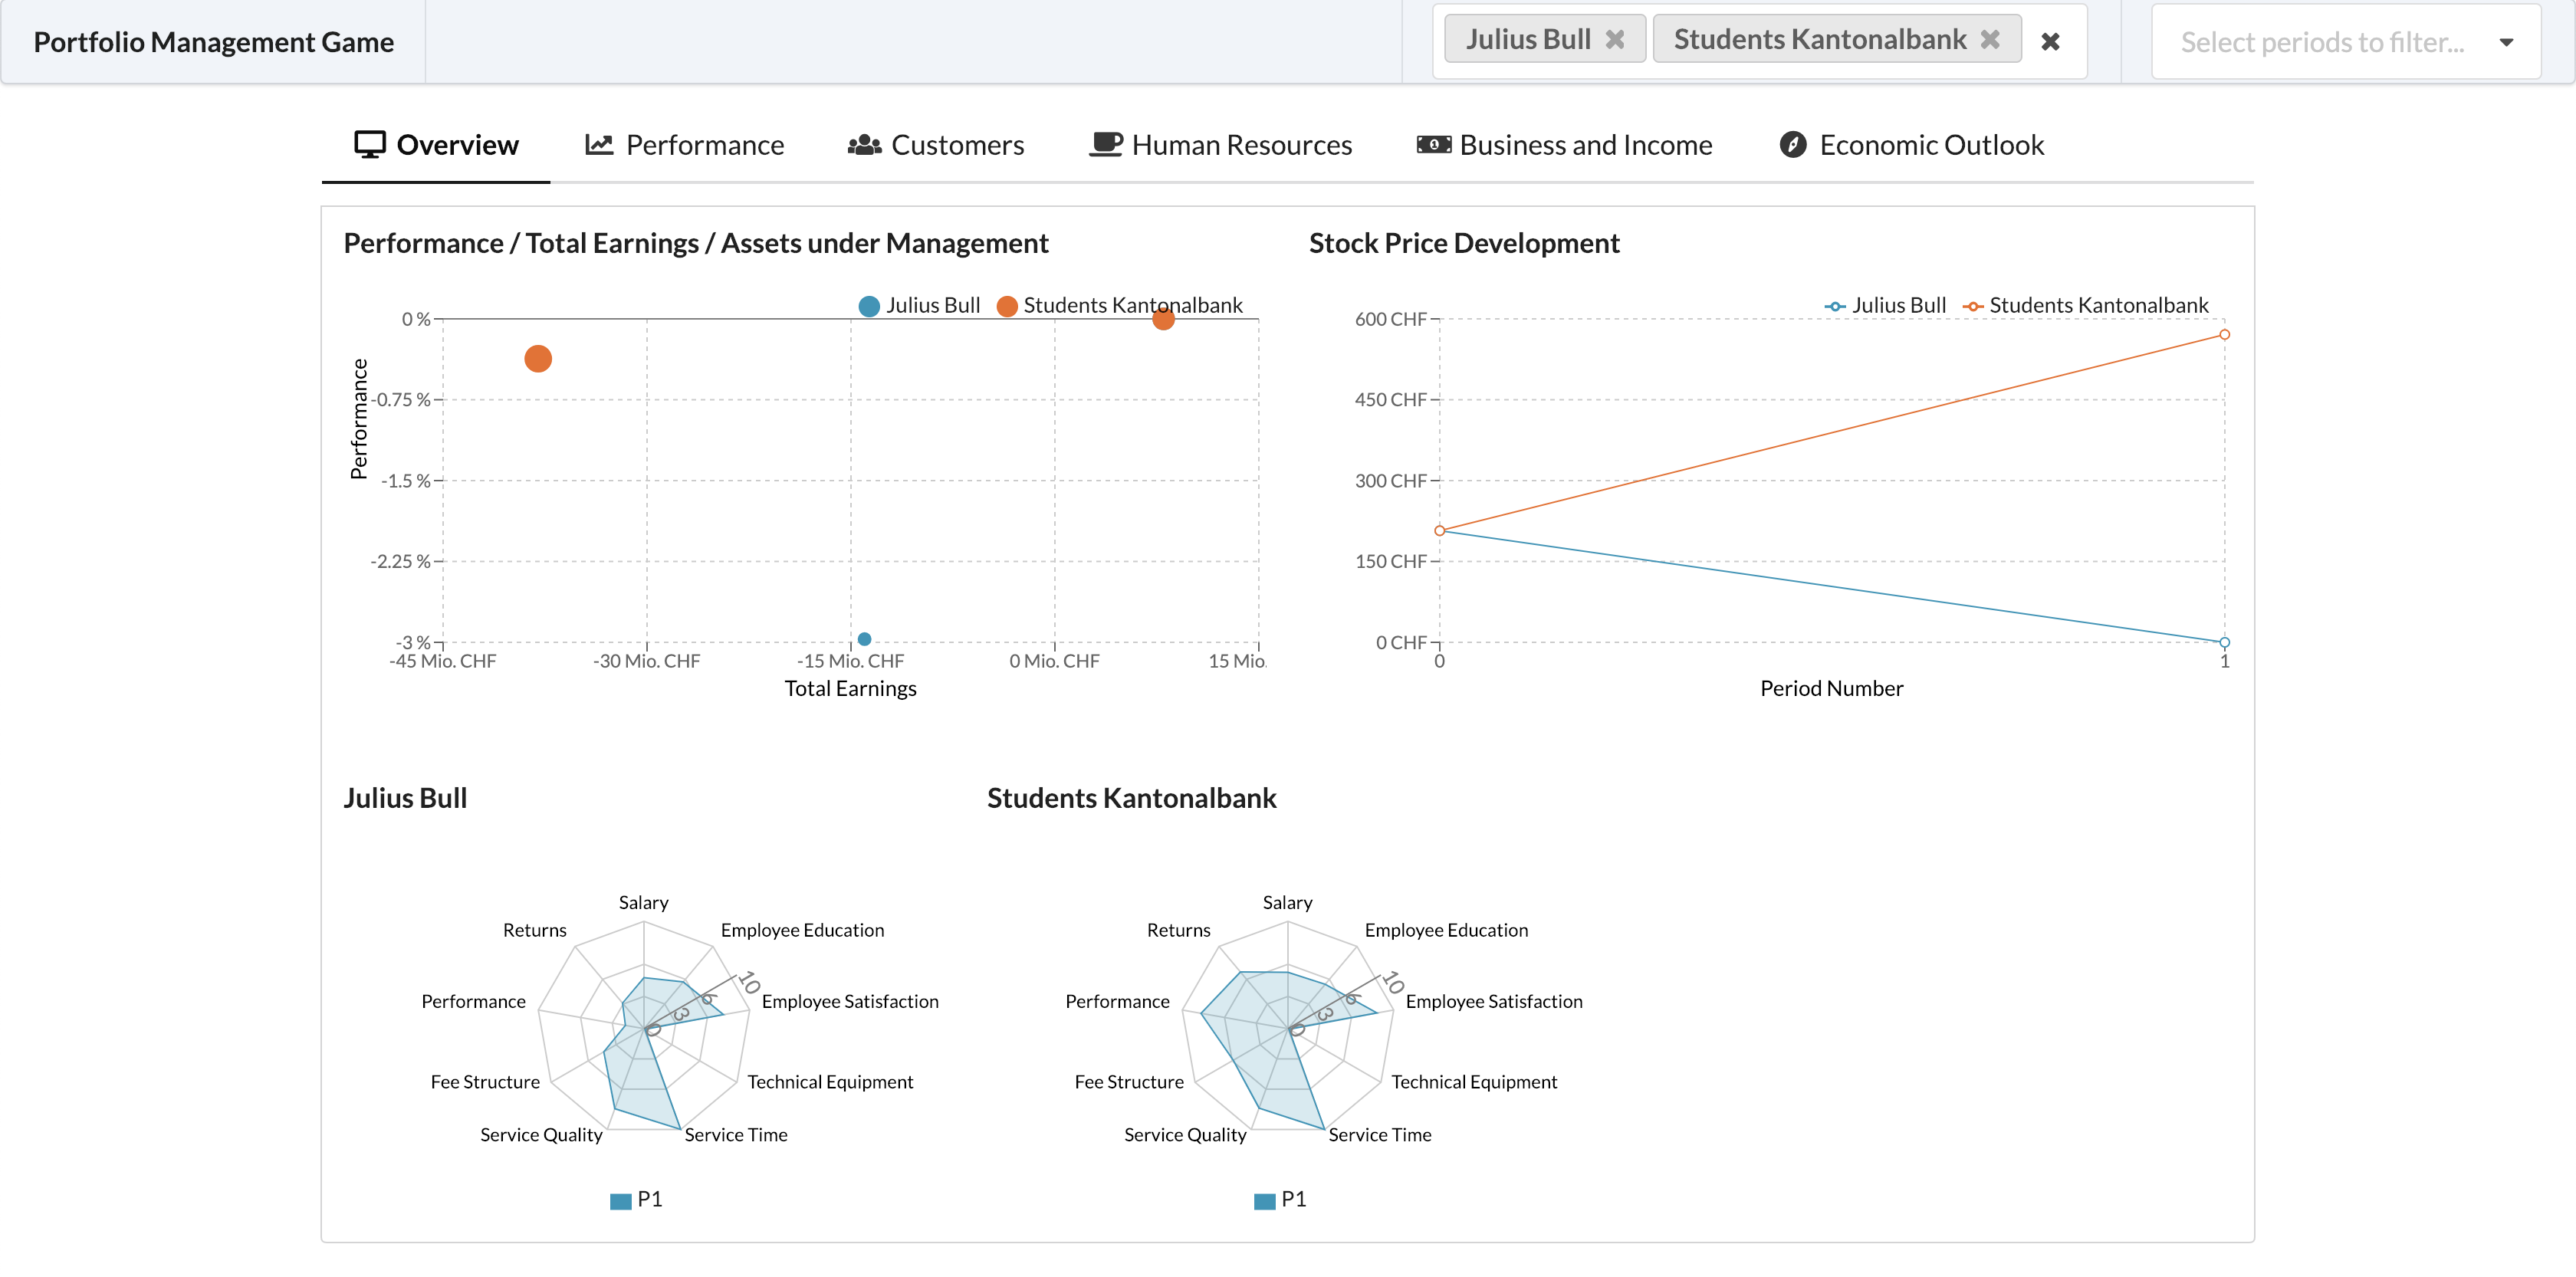
\includegraphics[scale=0.2]{img/application-overview/reports/01_overview.png}
  \caption{Reports - Overview}
\end{figure}

\subsubsection{Performance}
Multiple bar charts describe the performance of the teams for each customer type in each period. Such as:
\begin{itemize}
  \setlength\itemsep{0.01em}
  \item Portfolio returns
  \item Sharpe ratio
  \item Traynor ratio
  \item Jensen's alpha
  \item Information ratio
\end{itemize}
\begin{figure}[h!]
  \centering
  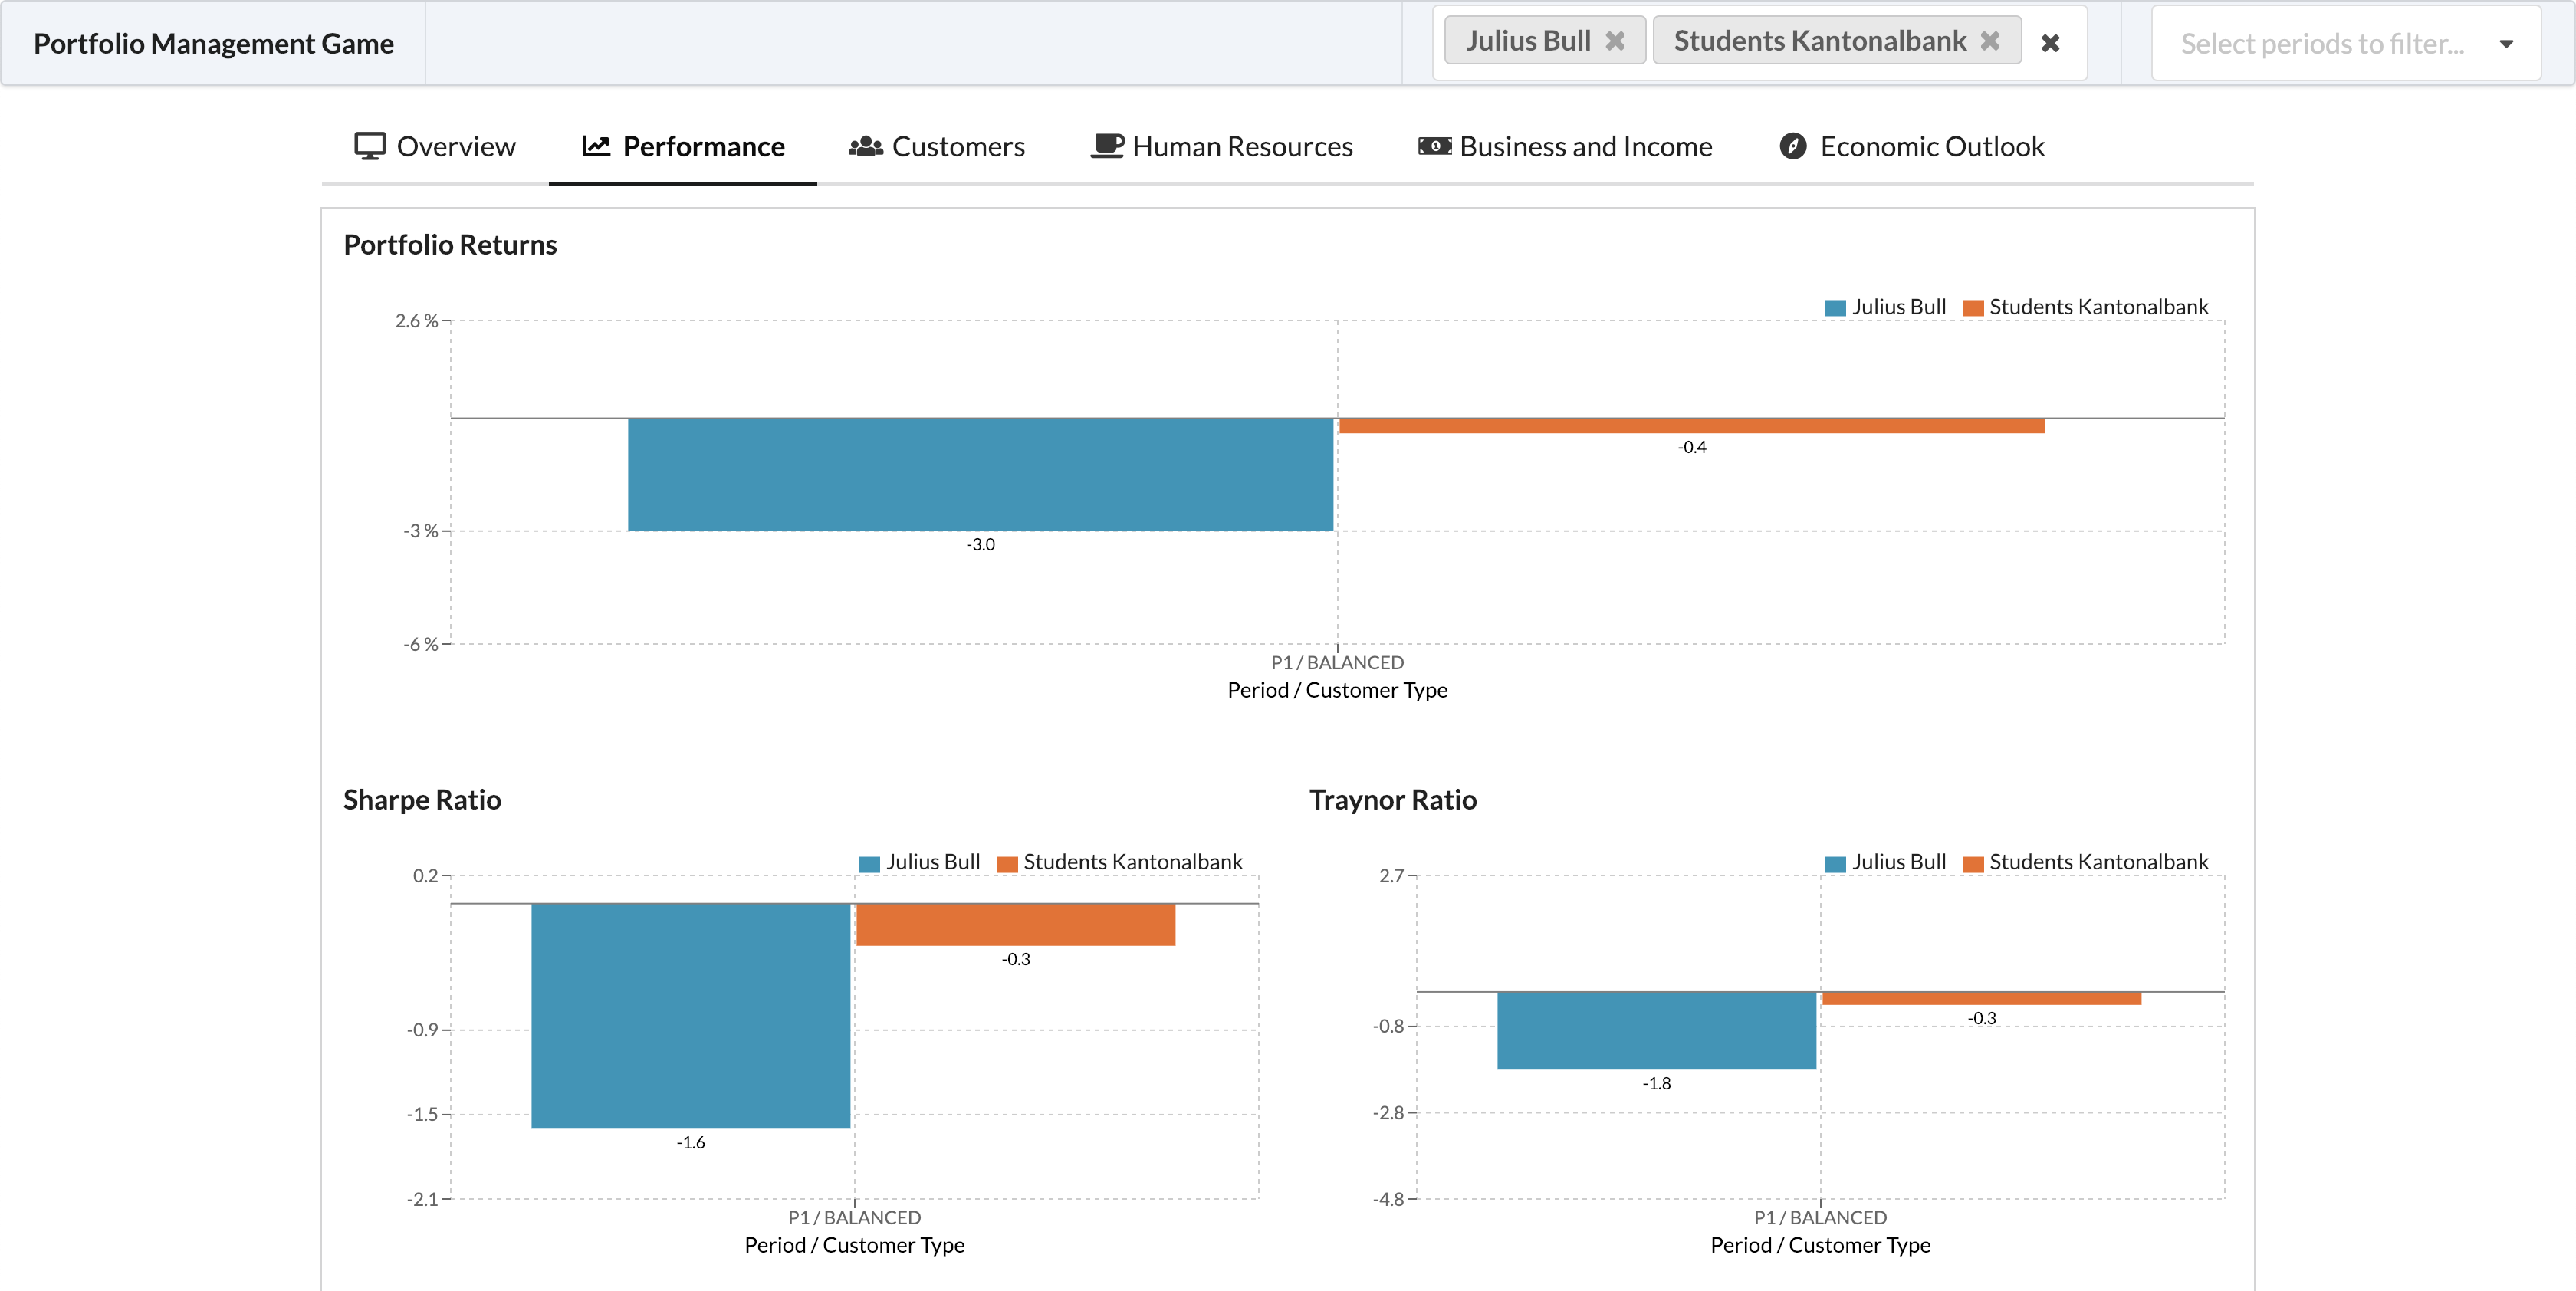
\includegraphics[scale=0.2]{img/application-overview/reports/02_performance.png}
  \caption{Reports - Performance}
\end{figure}

\subsubsection{Customers}
Similar to the performance tab, the customer section explains multiple key characteristics of customers for each team and period.
\begin{itemize}
  \setlength\itemsep{0.01em}
  \item Customer satisfaction index
  \item Number of Customers
  \item Customer growth
  \item Assets under management
  \item Net new money
  \item Relative TAA discrepancy (volume-weighted)
  \item Number of SAA violations
\end{itemize}
\begin{figure}[h!]
  \centering
  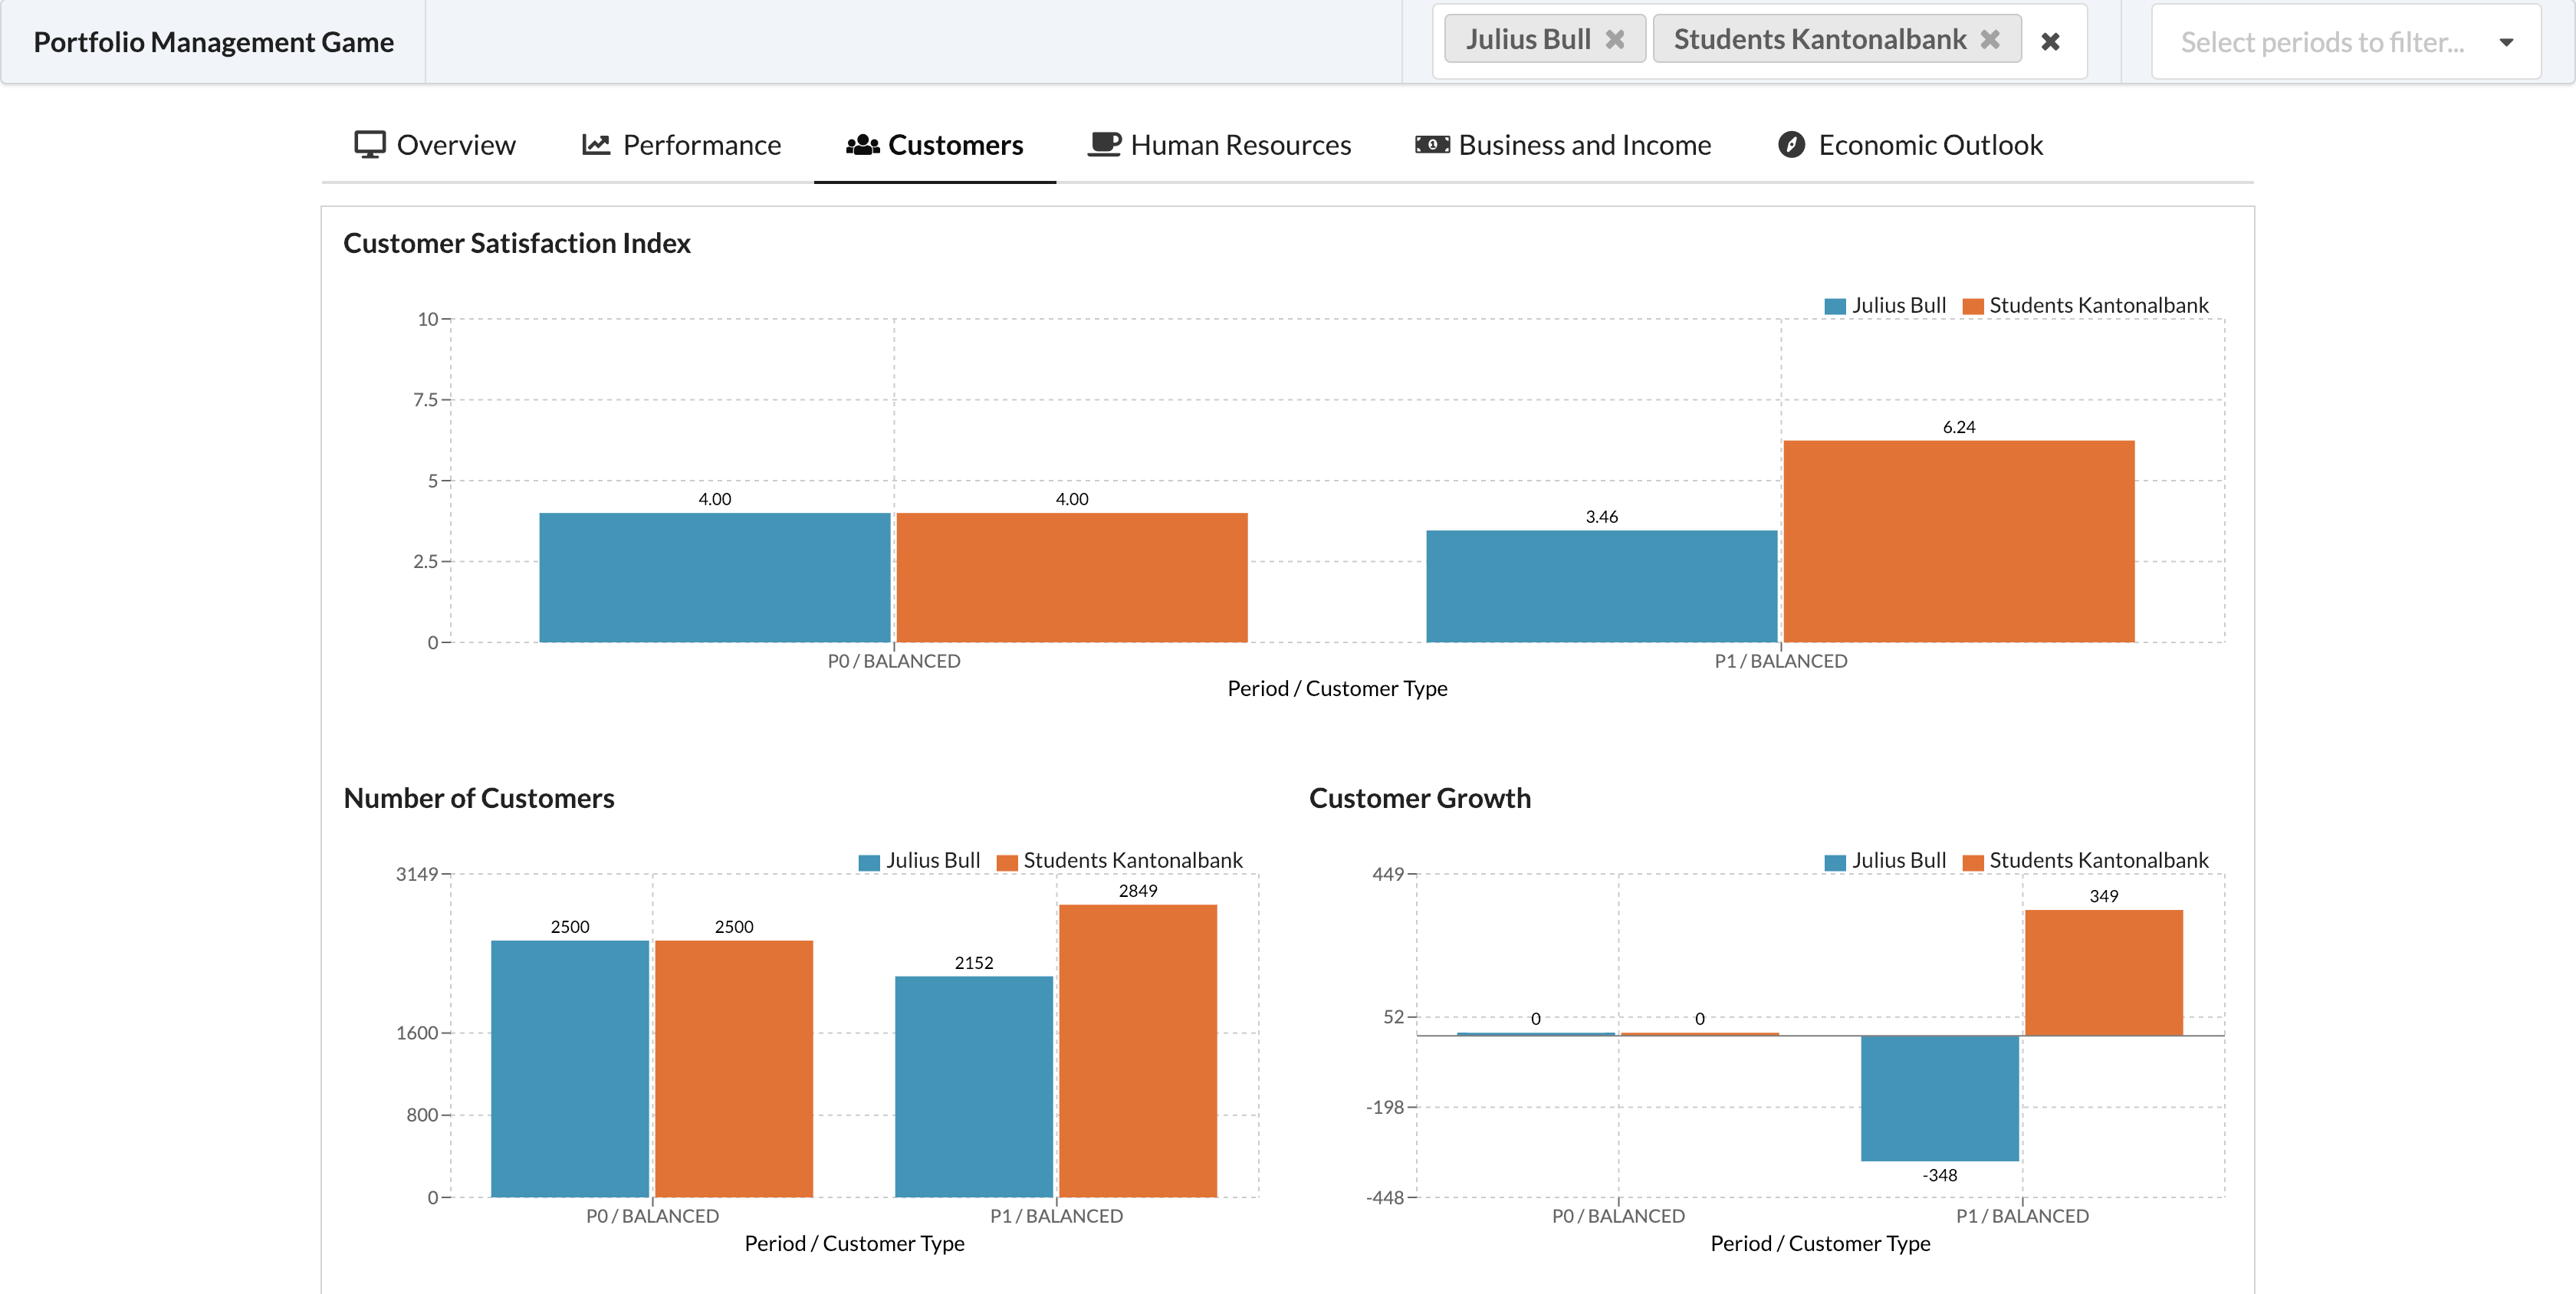
\includegraphics[scale=0.2]{img/application-overview/reports/03_customers.png}
  \caption{Reports - Customers}
\end{figure}

\subsubsection{Human ressources}
Information about human resources (HR) is displayed using four bar charts:
\begin{itemize}
  \setlength\itemsep{0.01em}
  \item Employee satisfaction index
  \item Number of employees
  \item Salary index
  \item Education index
\end{itemize}
\begin{figure}[h!]
  \centering
  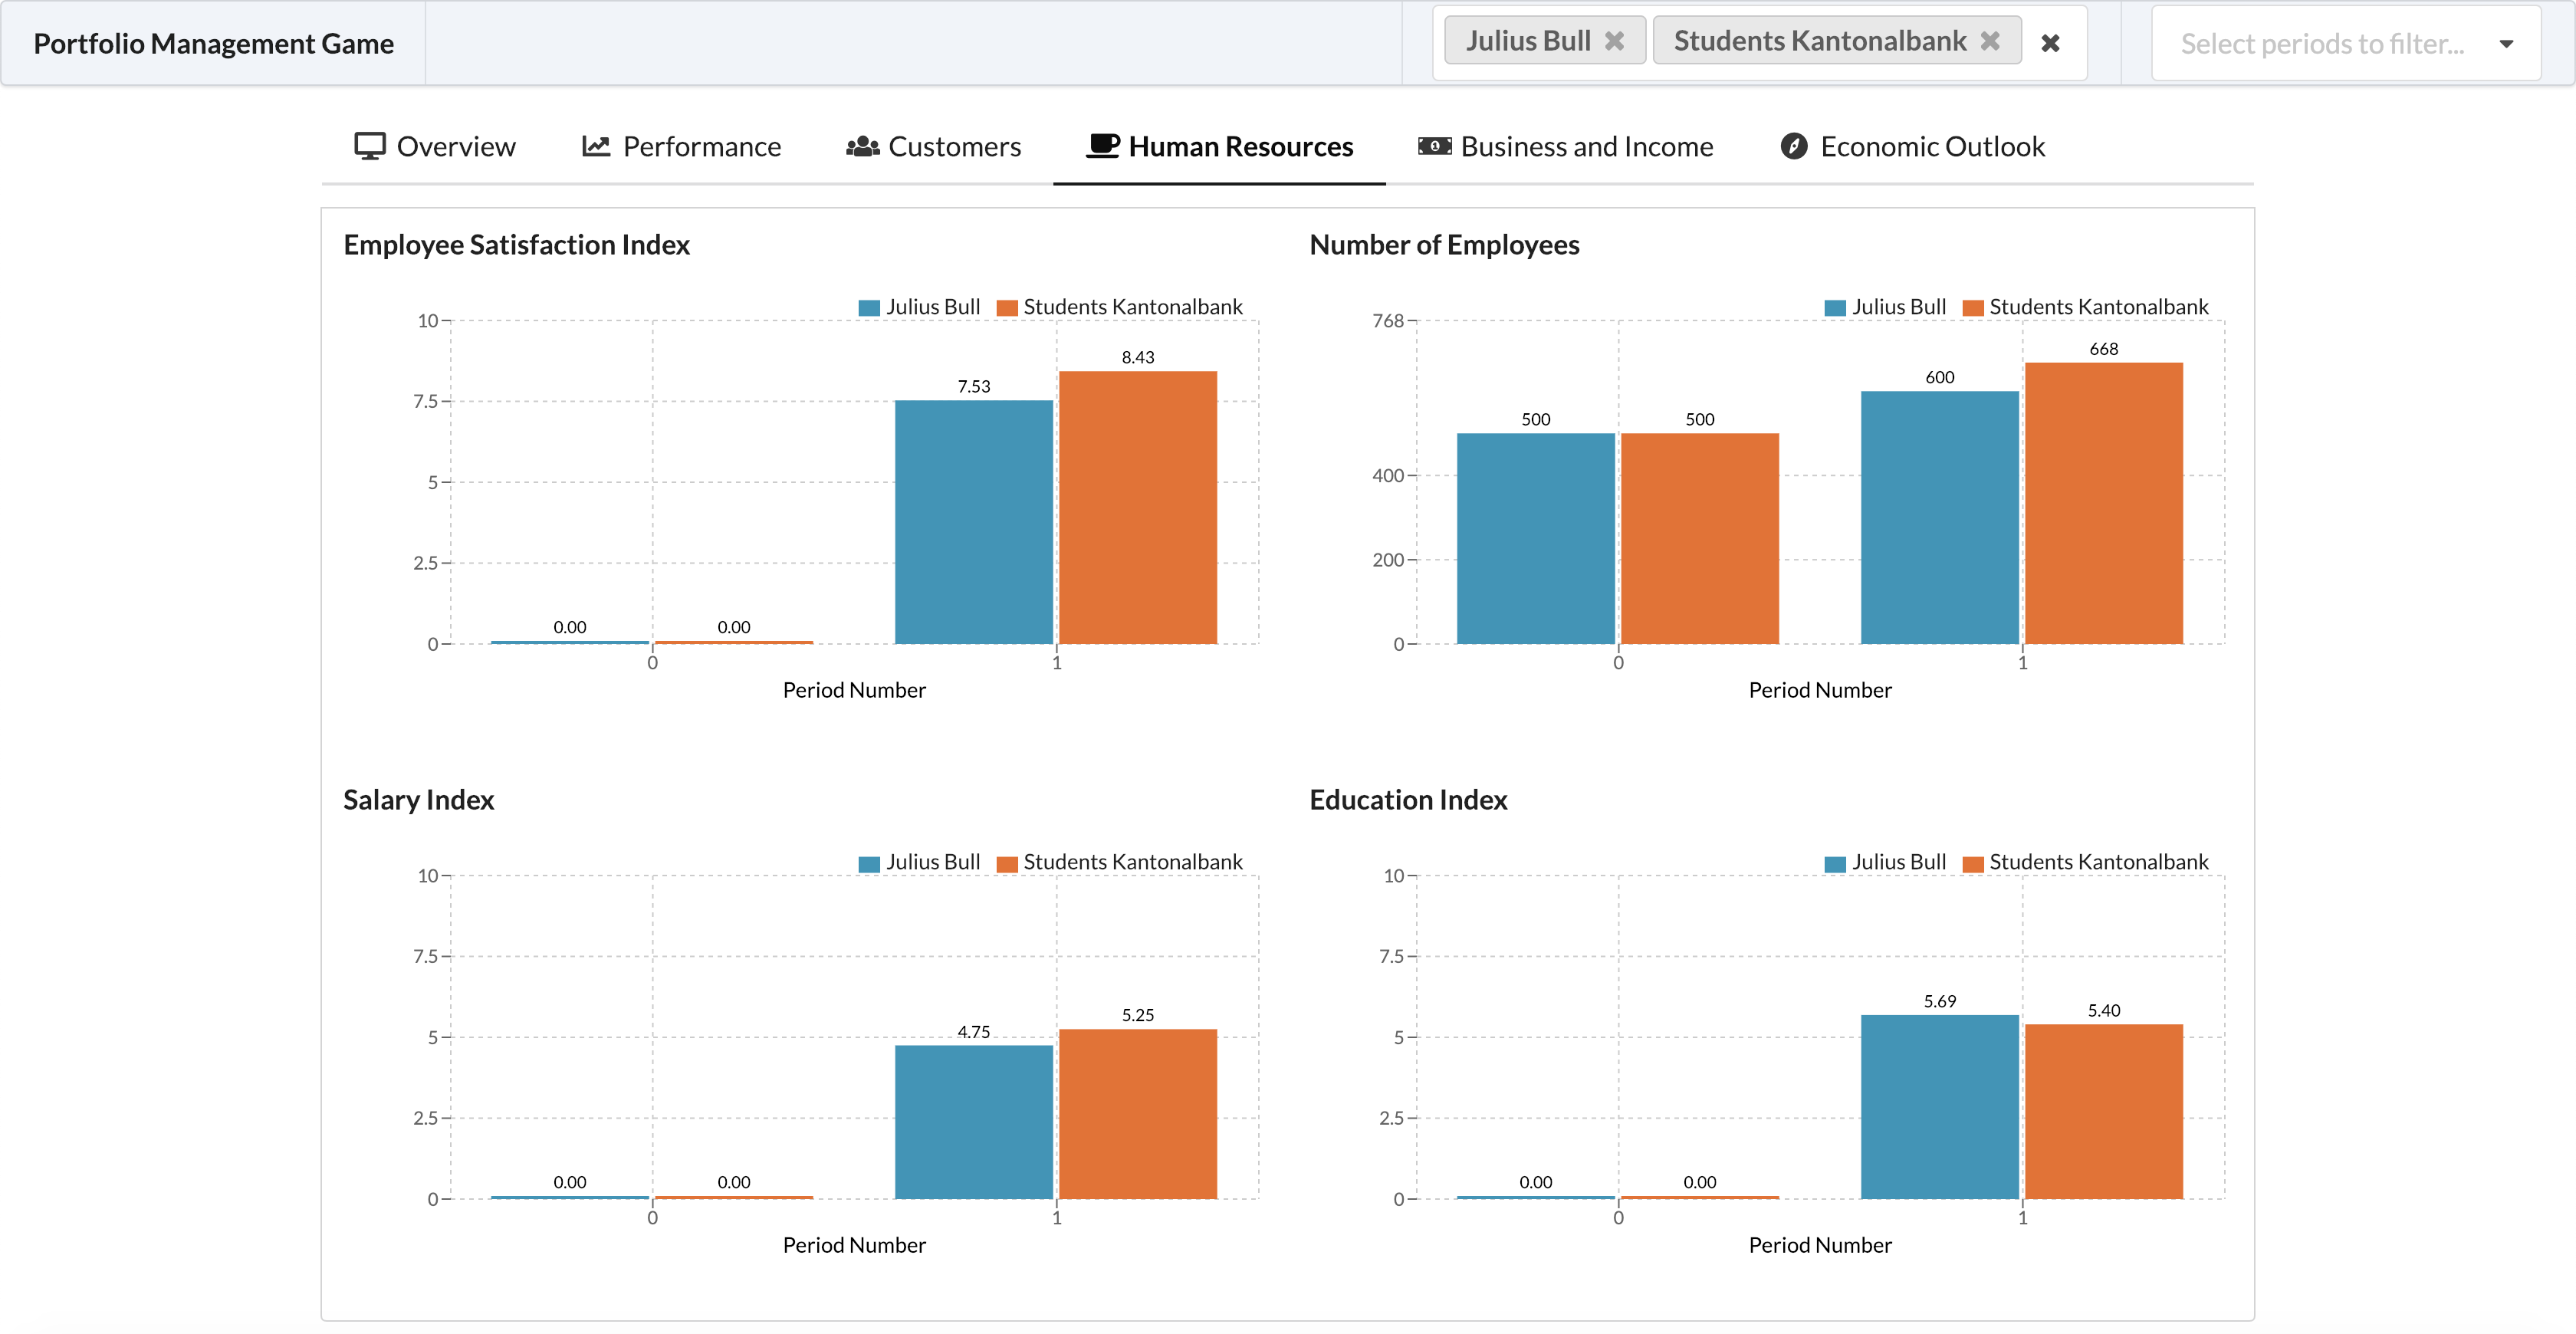
\includegraphics[scale=0.2]{img/application-overview/reports/04_hr.png}
  \caption{Reports - Human ressources}
\end{figure}

\subsubsection{Business and Income}
Starting with four bar charts this tab explains about business decisions:
\begin{itemize}
  \setlength\itemsep{0.01em}
  \item Operating Income
  \item Operating expenses
  \item Cost income ratio
  \item Net Income
\end{itemize}
\begin{figure}[h!]
  \centering
  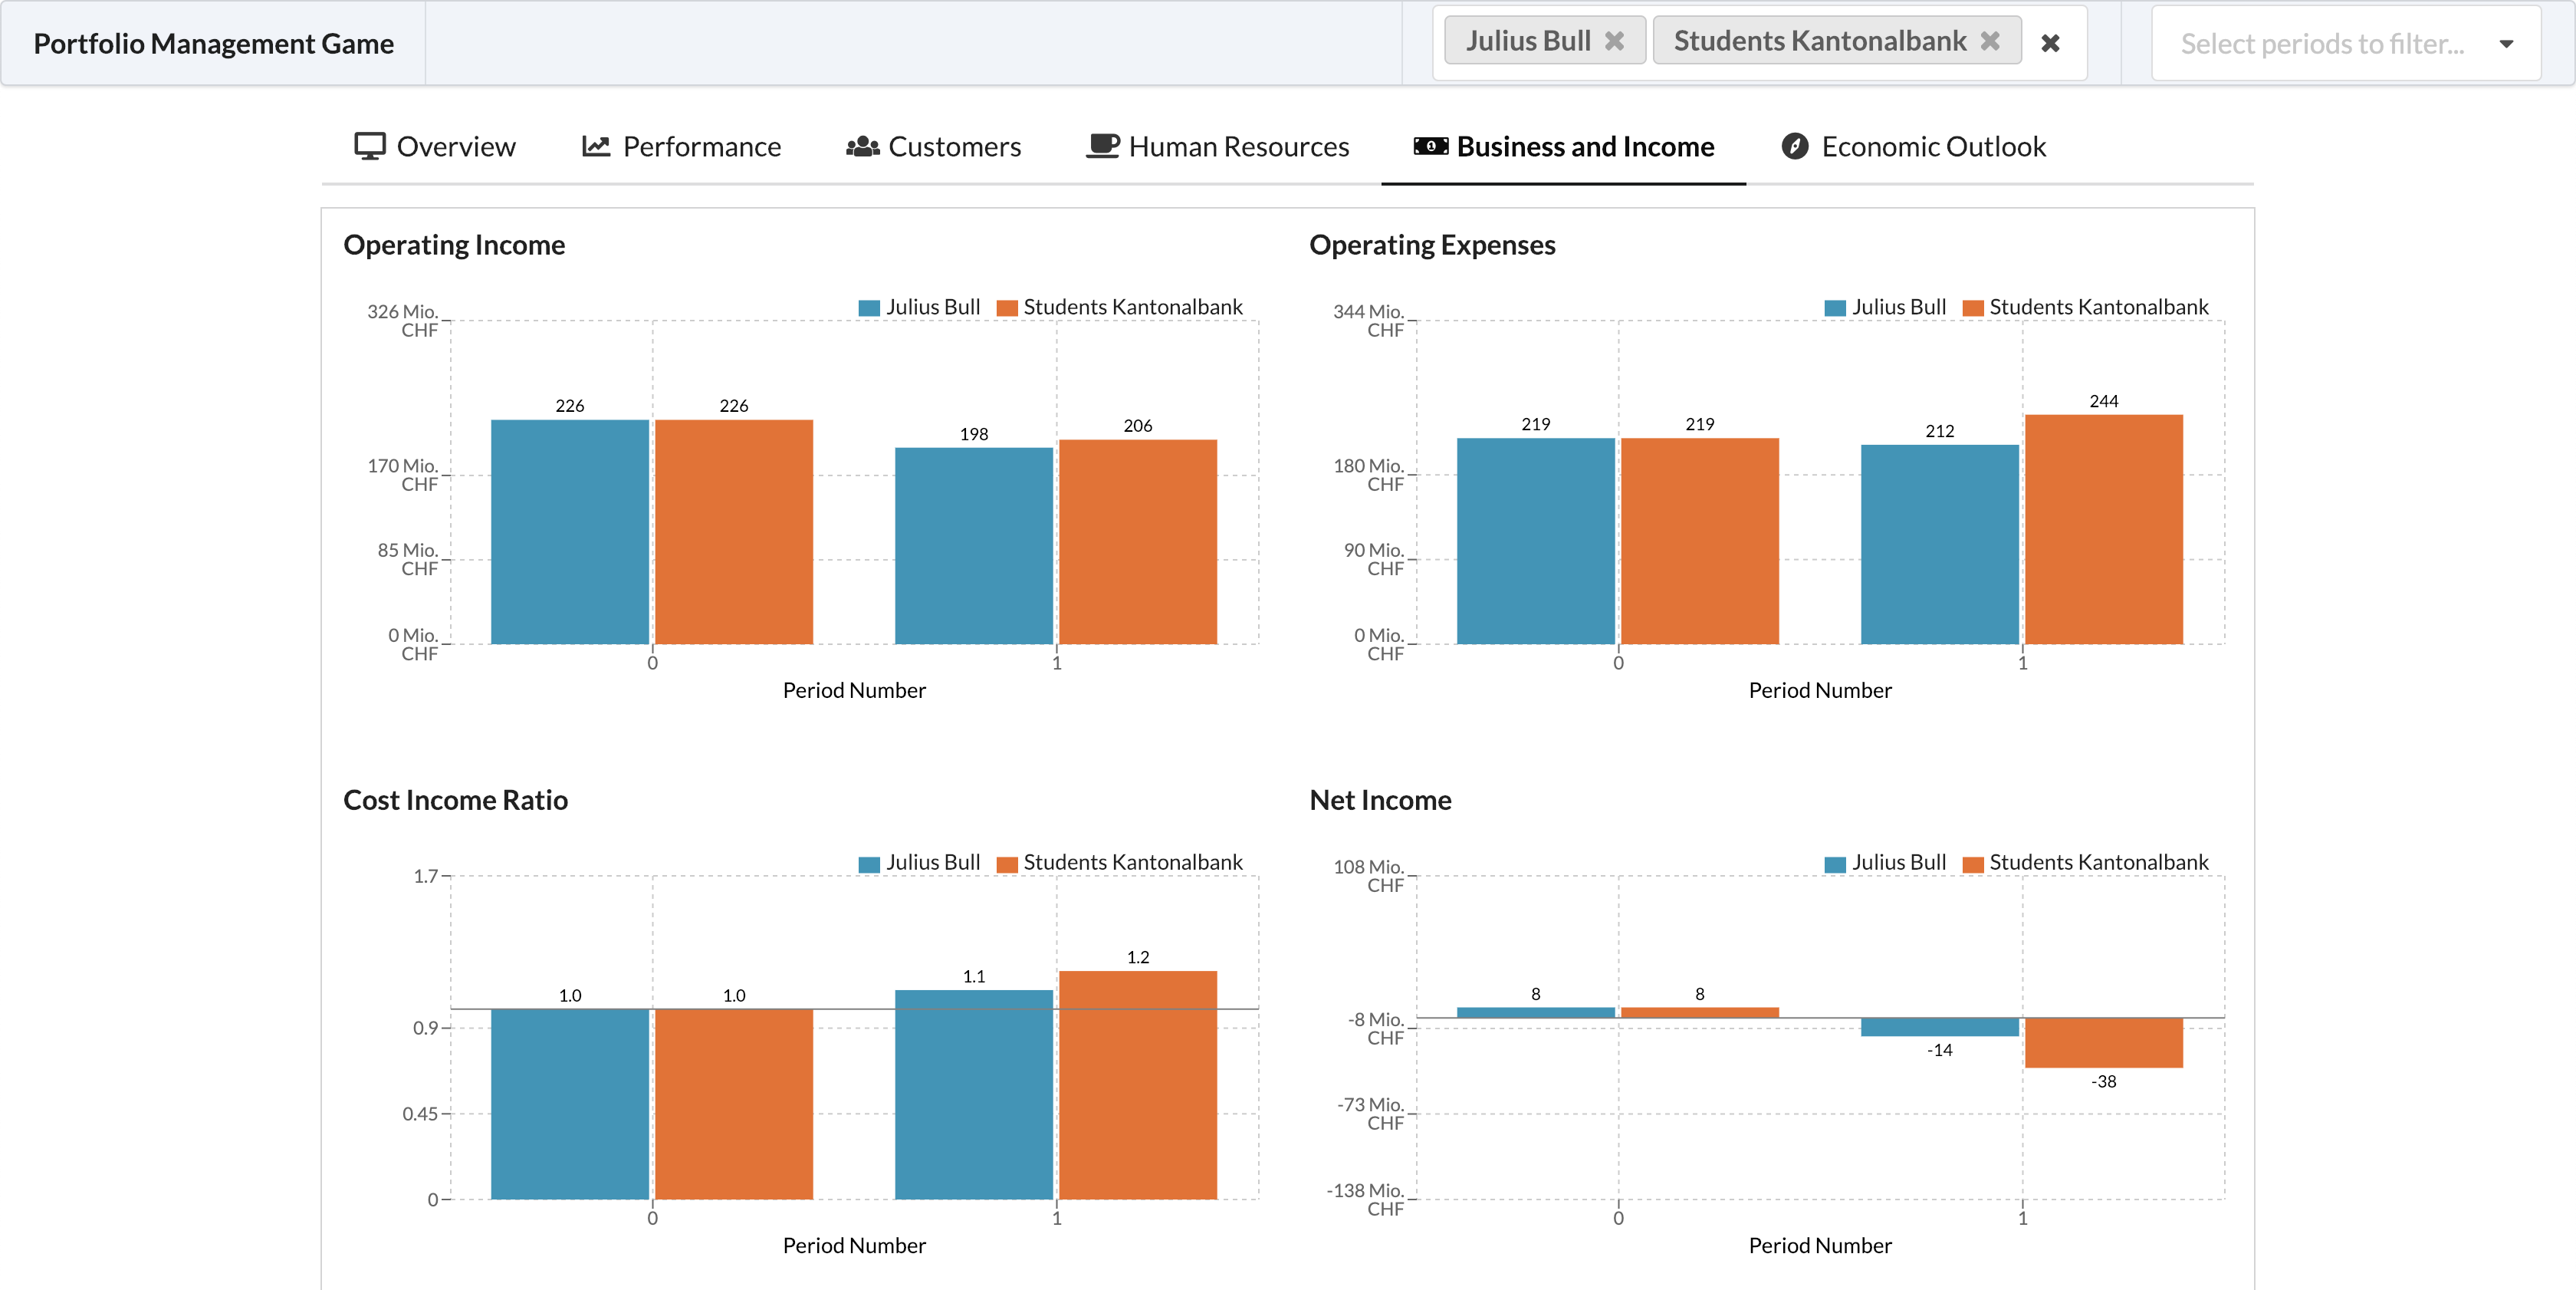
\includegraphics[scale=0.2]{img/application-overview/reports/05_business_income.png}
  \caption{Reports - Business and Income}
\end{figure}

In figure~\ref{fig:reports_balance_sheet_comparison} different teams in different periods can be compared for their balance sheet. The users can either compare previous periods with upcoming of their own balance sheet or compare their own result to other teams in the same period.
\begin{figure}[h!]
  \centering
  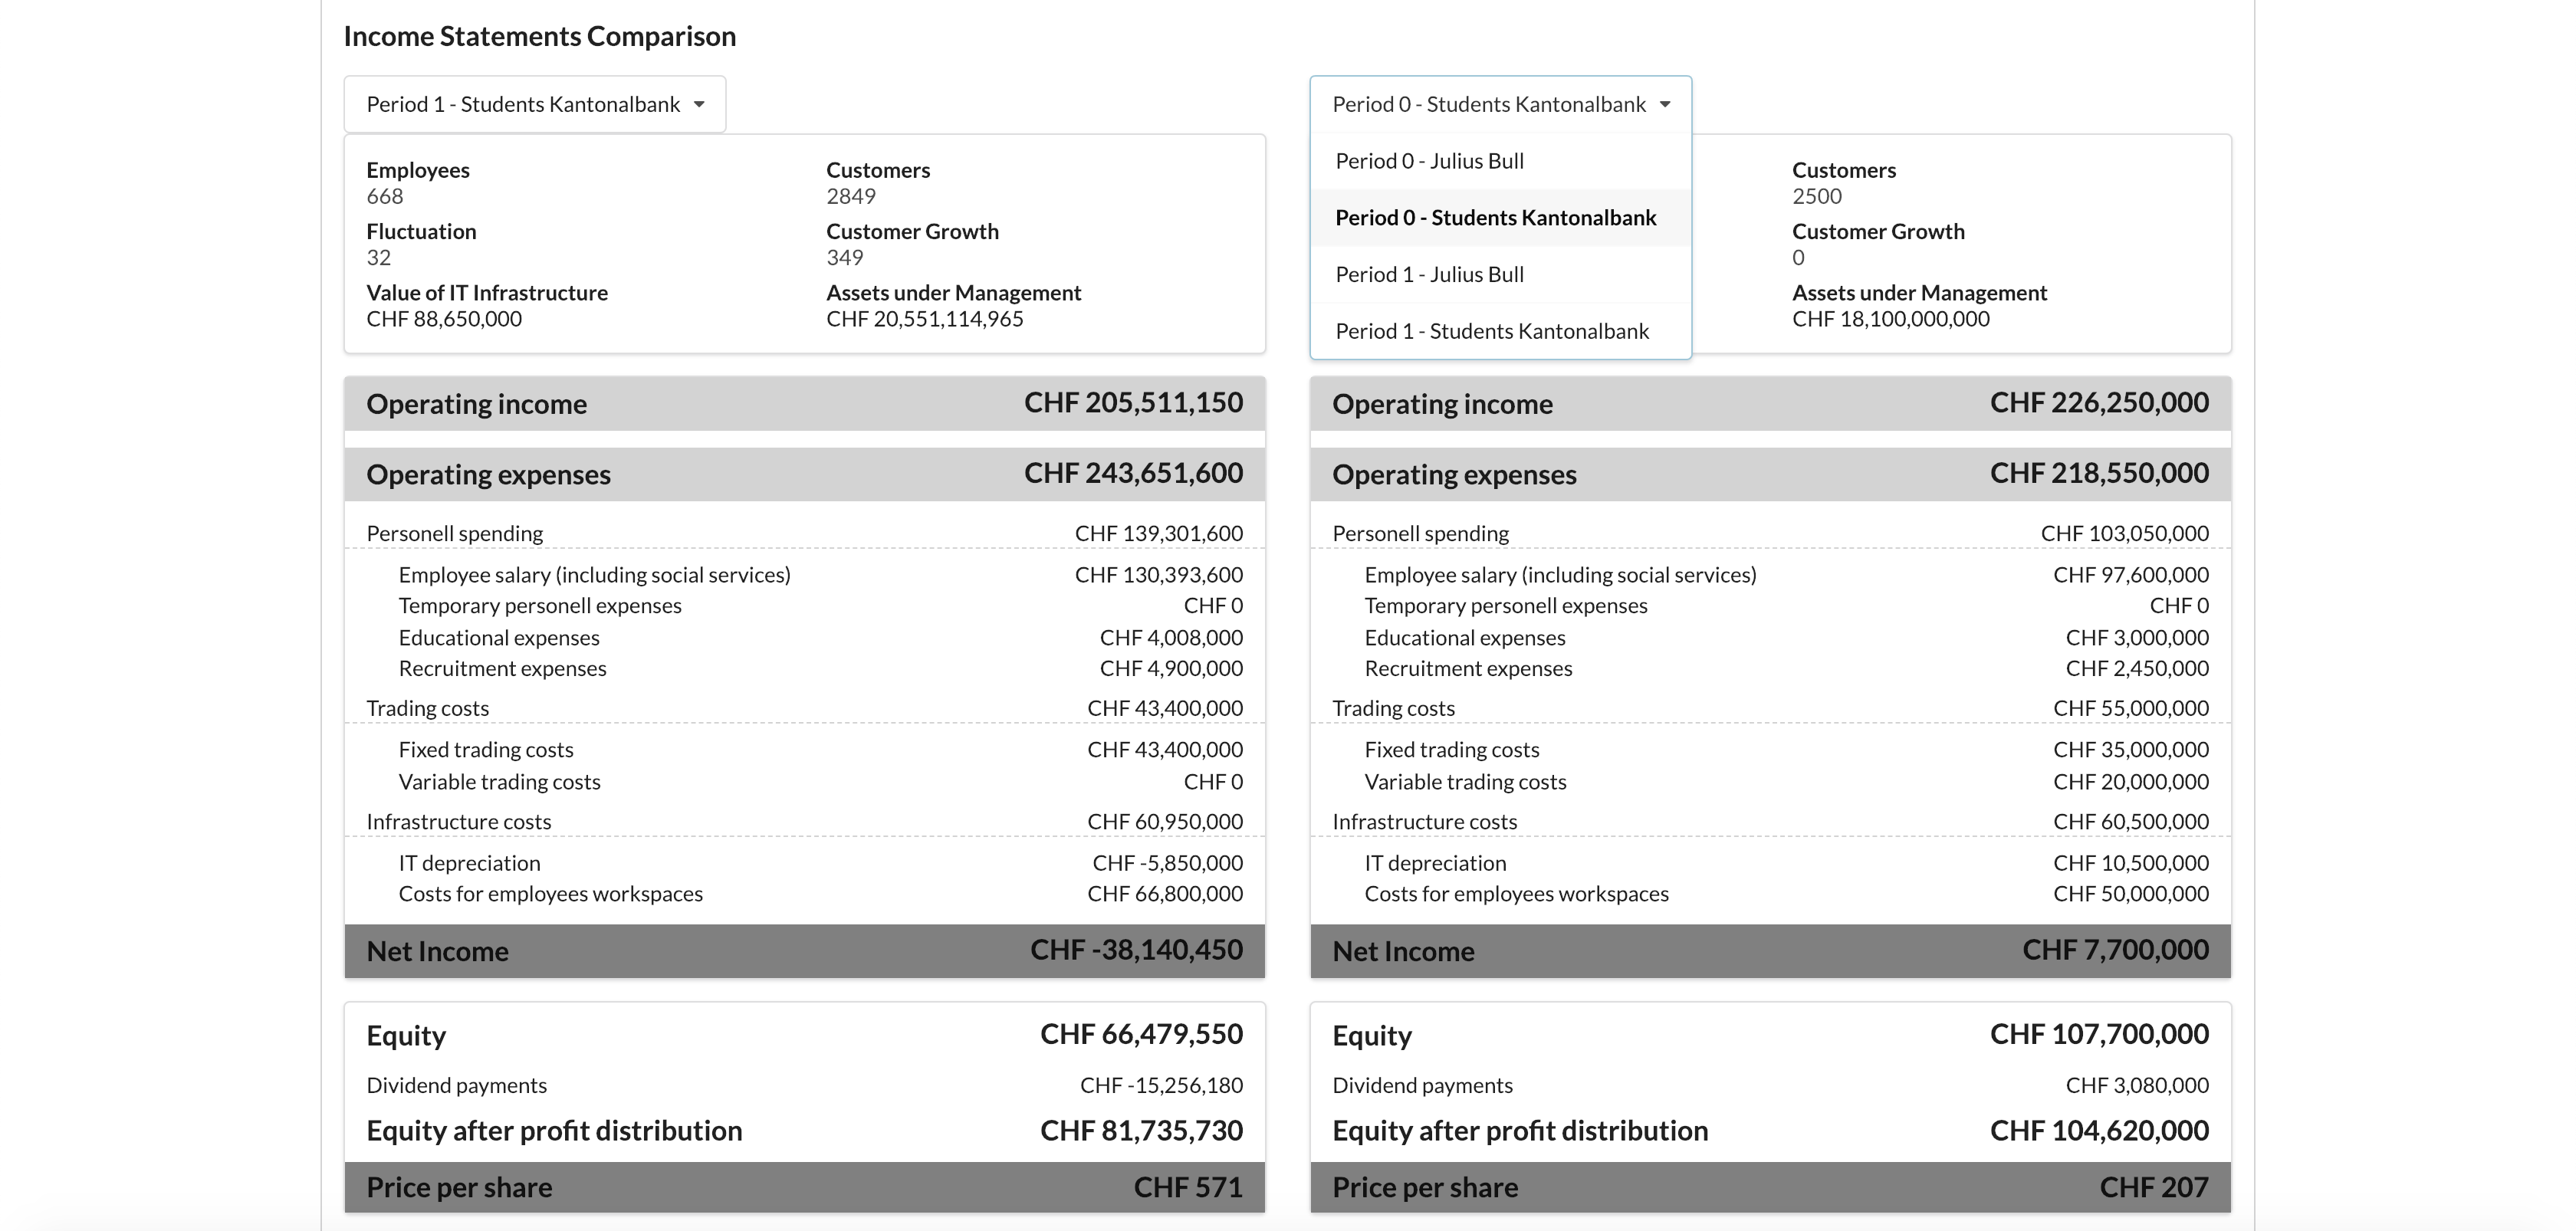
\includegraphics[scale=0.2]{img/application-overview/reports/05_business_income_balance_sheet_comparison.png}
  \caption{Reports - Balance sheet comparison}
  \label{fig:reports_balance_sheet_comparison}
\end{figure}


\subsubsection{Economic Outlook}
The economic outlook is the only tab, which is already accessible from period 1, as all other graphs or tabs have to be in at least period 2 because the first actual decisions (except for the saa) take place in period 1.
\begin{figure}[h!]
  \centering
  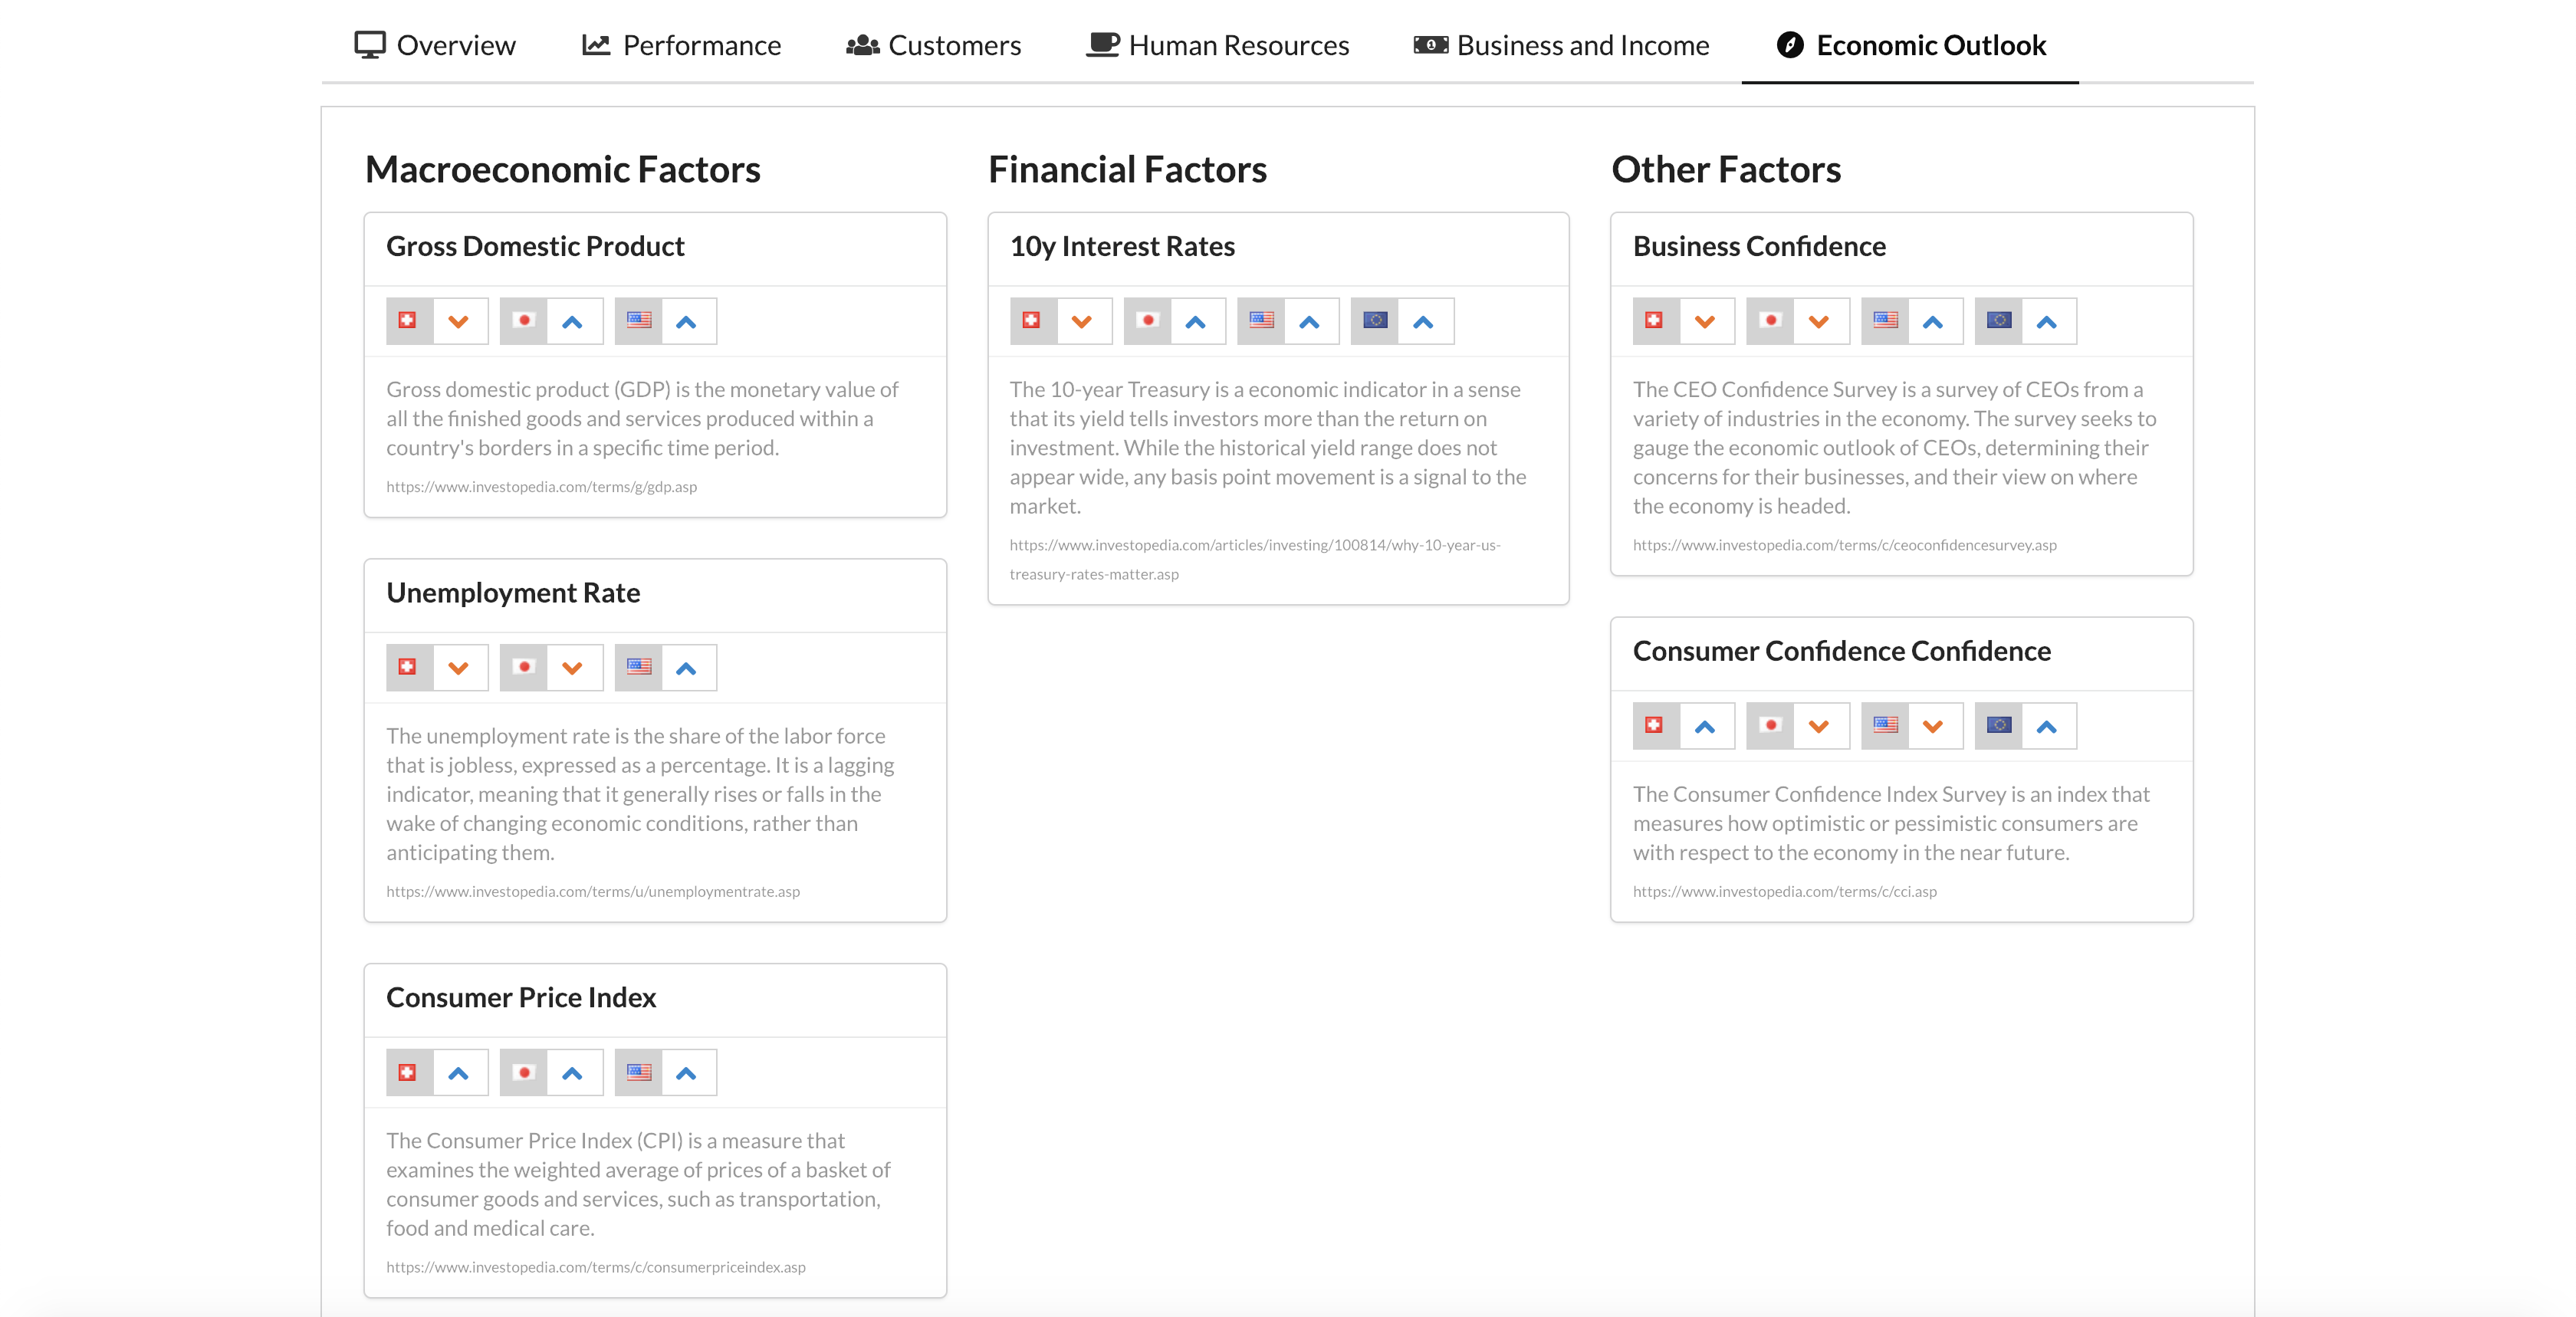
\includegraphics[scale=0.2]{img/application-overview/reports/06_economic_outlook.png}
  \caption{Reports - Economic outlook}
\end{figure}


\clearpage
\section{Conclusion}

\subsection{Current Progress}

...

\subsection{Future Development}

...

In the scope of the Master project, the project team has set up an initial game which is executable and testable for various settings including multiple teams per game and the most important administrator features. As the project was accompanied by a project planning tool called ''Trello'', there have been a lot of future tasks which may be implemented in the future but weren't planned within the scope of this Master project. The most epic features will be described in the following paragraph. \\

As not enough data for a bootstrapped game was provided, the authors focused on developing a game which will be played with historical data. The game is easily extendable for this purpose, as the initial plan was to set up both modes. The authors had to revise this plan due to the lack of provided data. When creating a game the administrator can choose the game type which is either a bootstrapped or a historical game. \\

% TODO more epic feature improvements

The project's plan is being ready for a first real game-execution by the Executive education's final seminar which will be held in July 2019. Additionally to the current courses where the application was used (as described in a previous chapter), the Department of Banking and Finance plans to set up another execution for the assessment course ''Banking and Finance II'', in which 700 students would participate in. The effort of setting this up for such a large number of students would need a lot of stress testing for the application.


\newpage

\appendix
\section{User Stories}

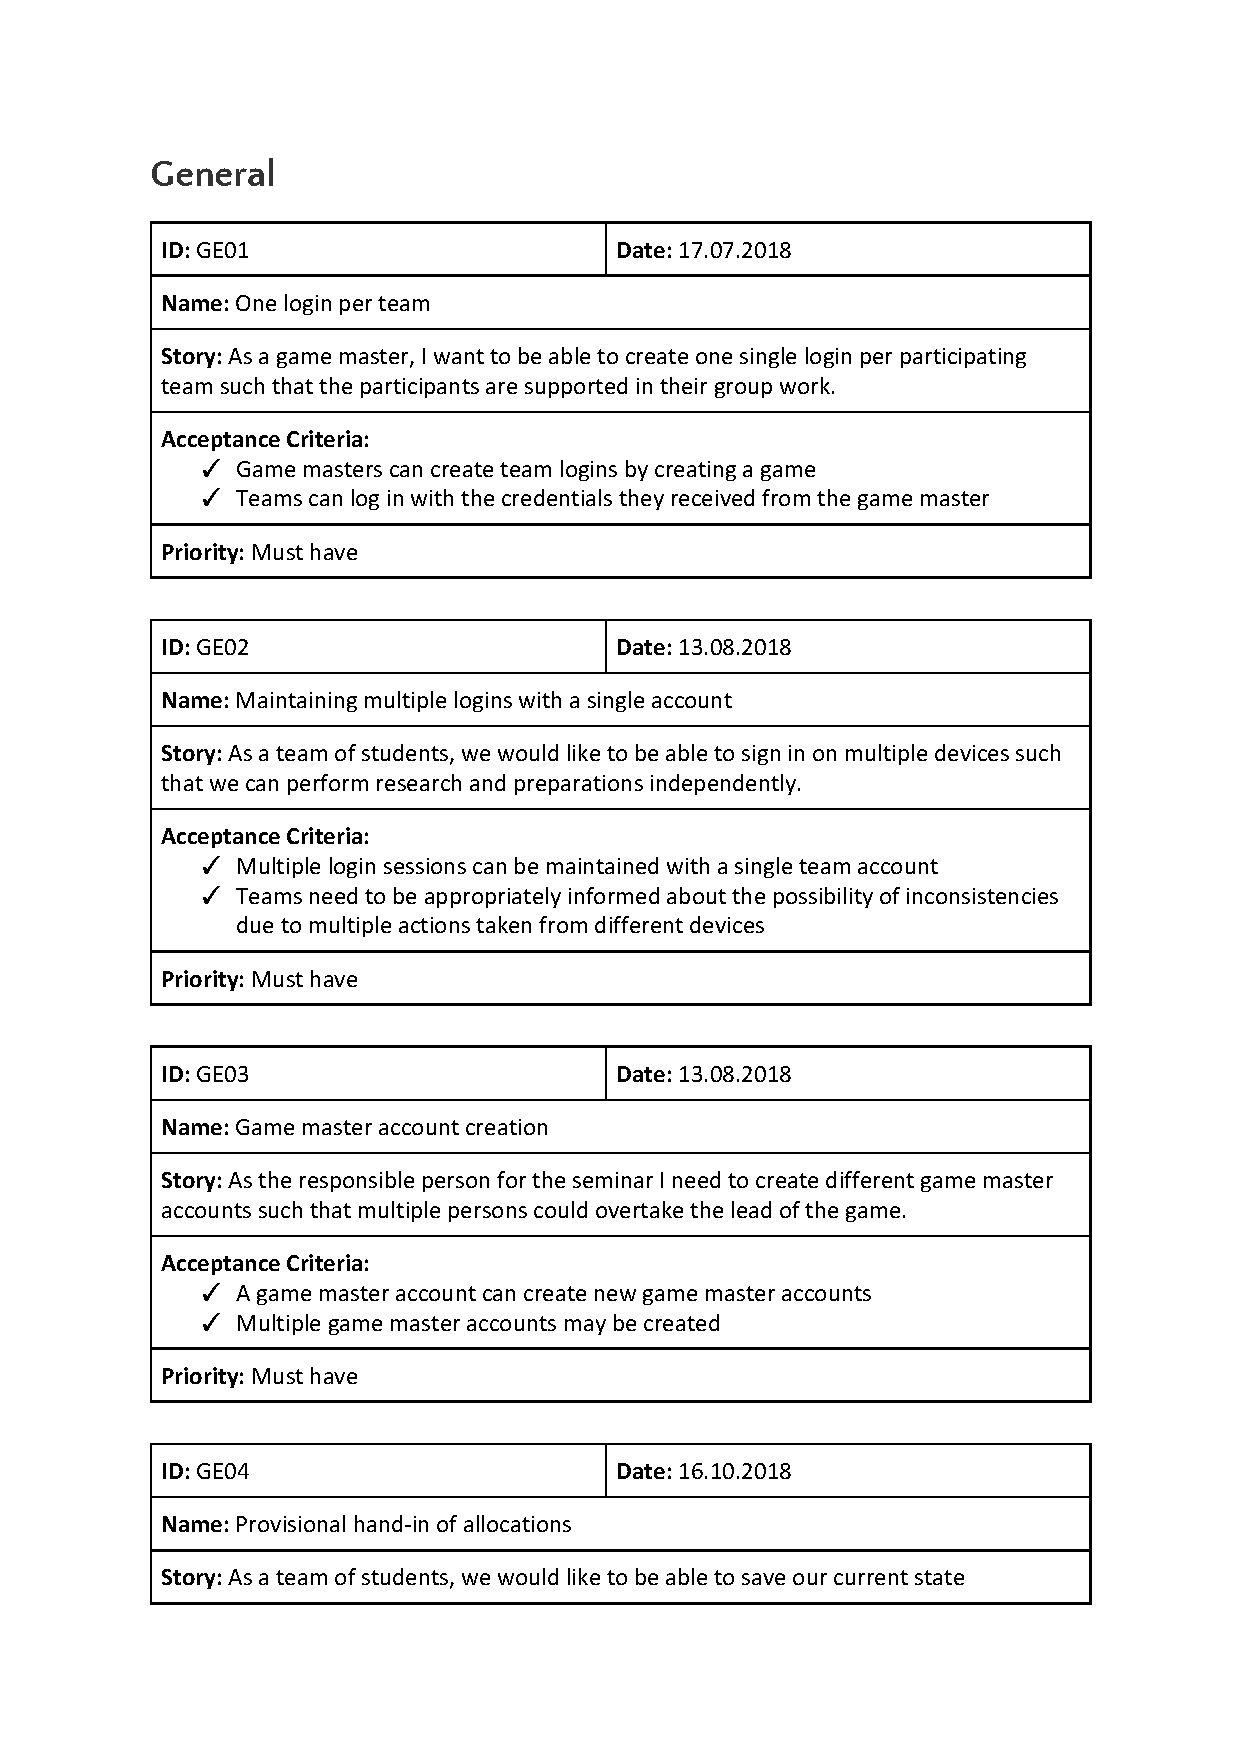
\includepdf[pages={-}, frame, delta=0 20]{appendix/user_stories.pdf}

\section{Interview Questions}
\label{sec:appendix_interview_questions}

\subsection{Data Collection Template}

\paragraph{What method do you plan to collect data?}
\begin{itemize}
  \item Interview along the lines of previously prepared questions in a semi-structured way
  \item Focus on materials as far as they can be provided by the professionals (screenshots, etc.)
  \item Focus on their decision and thought process while performing their professional work
  \item Discussion about their experience with the current state of the game, as far as they have used or seen the current game (additional requirements, didactical potential, etc.)
\end{itemize}

\paragraph{Possible Questions}
\begin{itemize}
  \item Shortly describe what you do in your daily professional work? How are you involved with portfolio management (more concretely)?
  \begin{itemize}
    \item Idea: get to know the big picture
  \end{itemize}
  \item How do you typically go about starting a new project (i.e., create a portfolio for a new customer)?
  \begin{itemize}
    \item Idea: get an intuition about the beginning of a new process
  \end{itemize}
  \item Does your portfolio management process follow a relatively consistent sequential path or do you often work on multiple tasks in parallel, switching back and forth?
  \begin{itemize}
    \item Idea: find out whether the current application is a suitable model of the professional process or whether a more sequential structure is more realistic
  \end{itemize}
  \item   Shortly elaborate on the main steps in your portfolio management workflow and try to use the terms Customer Contact, Research, SAA, TAA, Depot Realization, Performance Attribution.
  \begin{itemize}
    \item Idea: get them to talk about the steps in our current process and evaluate its appropriateness
    \item Find the practical differences to our current process (Customer Analysis, SAA, TAA, ,etc.)?
  \end{itemize}
  \item What tools do you use in your portfolio management process and how do you combine these tools?
  \begin{itemize}
    \item Idea: get an idea about their multitasking capabilities and necessities for context switching
    \item Excel, specific portfolio management tools (proprietary, etc.)
  \end{itemize}
  \item Are customers split into different “categories” like “risk-averse”, etc.? If yes, how do you decide about this categorization? And how do you define the reasonable “ranges” for any of these categories?
  \begin{itemize}
    \item Idea: find out whether the currently defined ranges are reasonable or whether they should be left out for the students to define themselves
  \end{itemize}
  \item When consulting with a new customer, do you define binding constraints like the Strategic Asset Allocation? If yes, can you deviate from these constraints? Do you adjust these constraints periodically?
  \begin{itemize}
    \item Idea: find out whether the approach of “locking” SAA for the remaining periods is reasonable
  \end{itemize}
  \item Do you hedge your investments in foreign currencies based on the profile and preferences of the client?
  \begin{itemize}
    \item Idea: find out whether the current approach to hedging makes sense
  \end{itemize}
\end{itemize}

\paragraph{How will you collect data?}
\begin{itemize}
  \item Audio recording (if consent) as well as notes
  \item Collect additional materials as far as possible (screenshots, etc.)
\end{itemize}

\paragraph{How do you plan to analyze the data?}
\begin{itemize}
  \item Create partial transcriptions with appropriate summarizations
  \item Create mind-maps and diagrams modeling a typical professional workflow
  \item Work towards a valid work model describing the professional interactions
  \item Improve and validate the models across multiple interviews
\end{itemize}

\paragraph{What will you plan to show in our August meeting as evidence of your findings?}
\begin{itemize}
  \item A presentation with process diagrams (as far as already possible)
\end{itemize}

\subsection{Interview Notes}
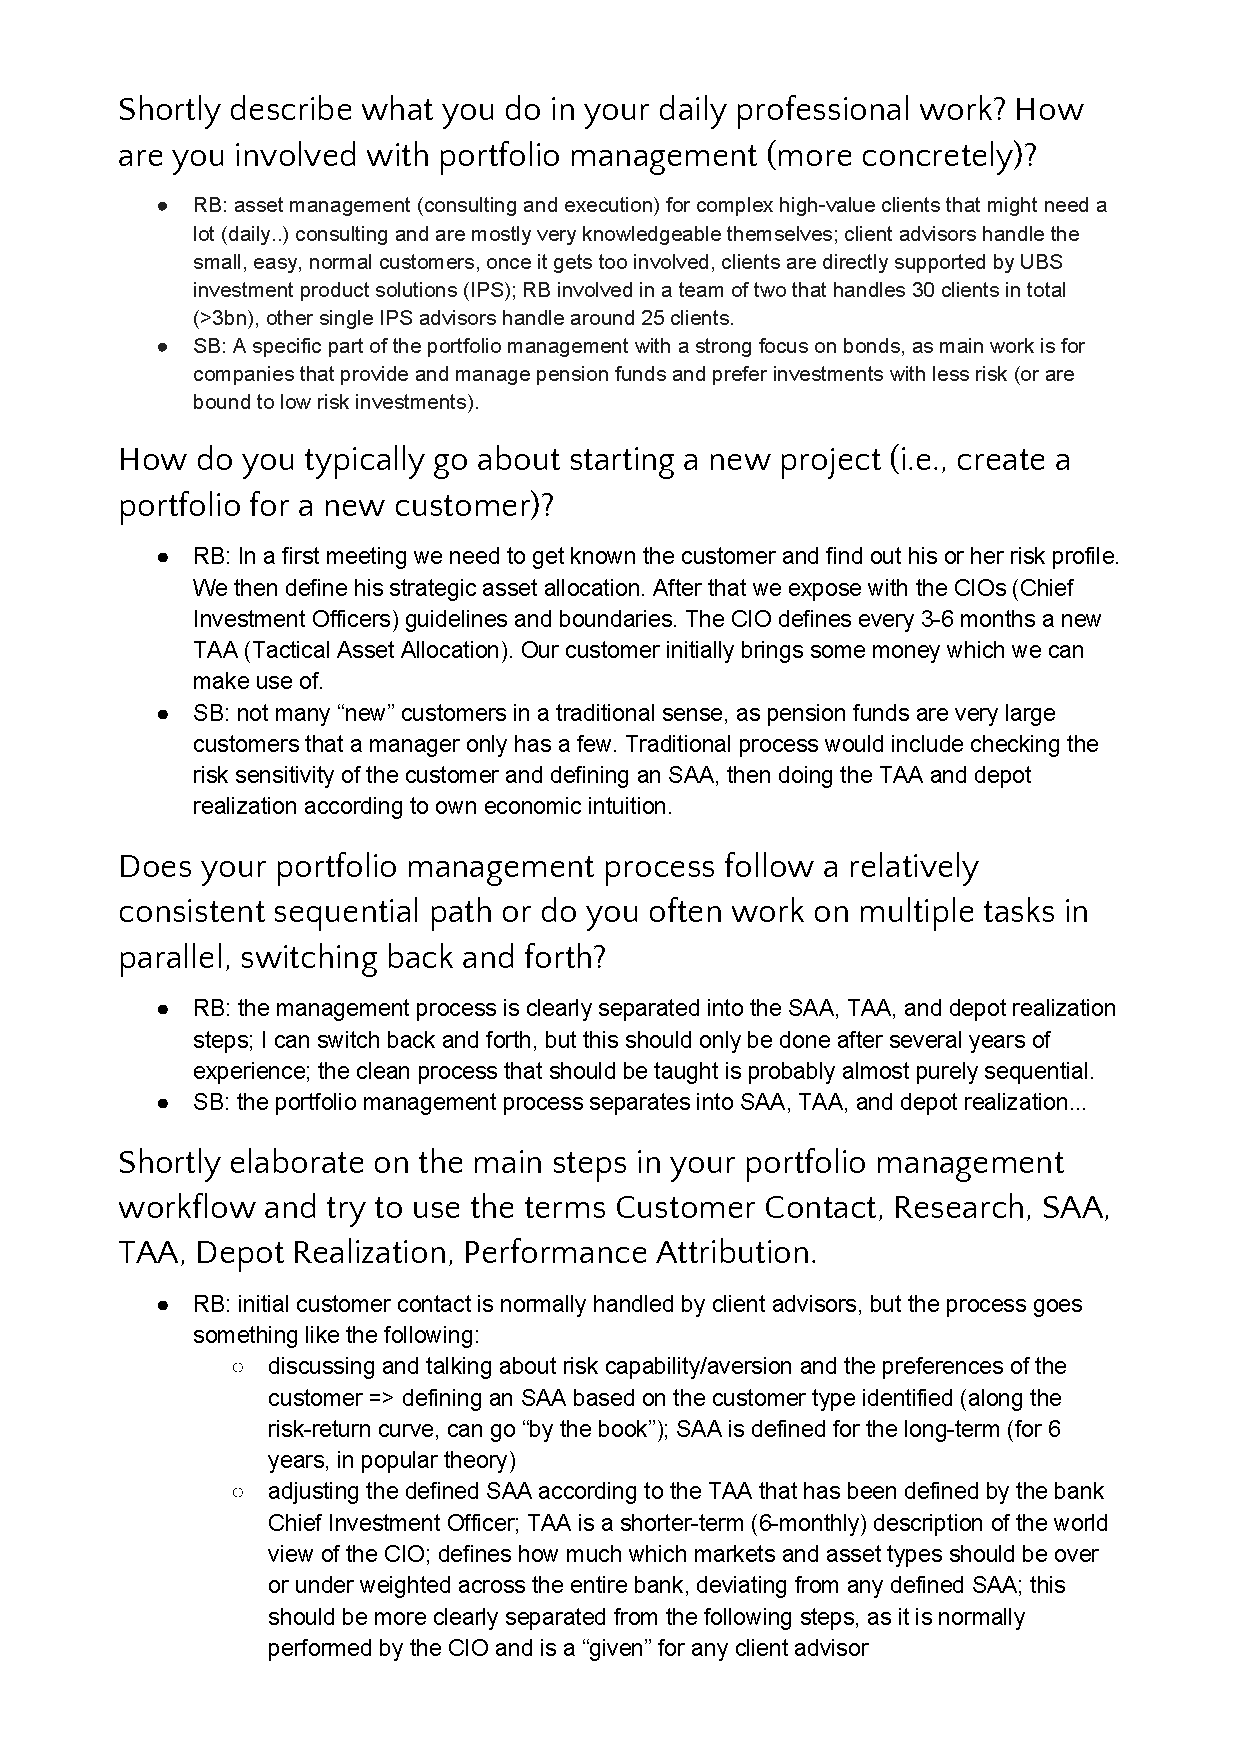
\includepdf[pages={-}, delta=0 20]{appendix/meeting_notes.pdf}

\section{Observation Notes}
\label{sec:appendix_observation_notes}
\begin{sidewaysfigure}[ht]
  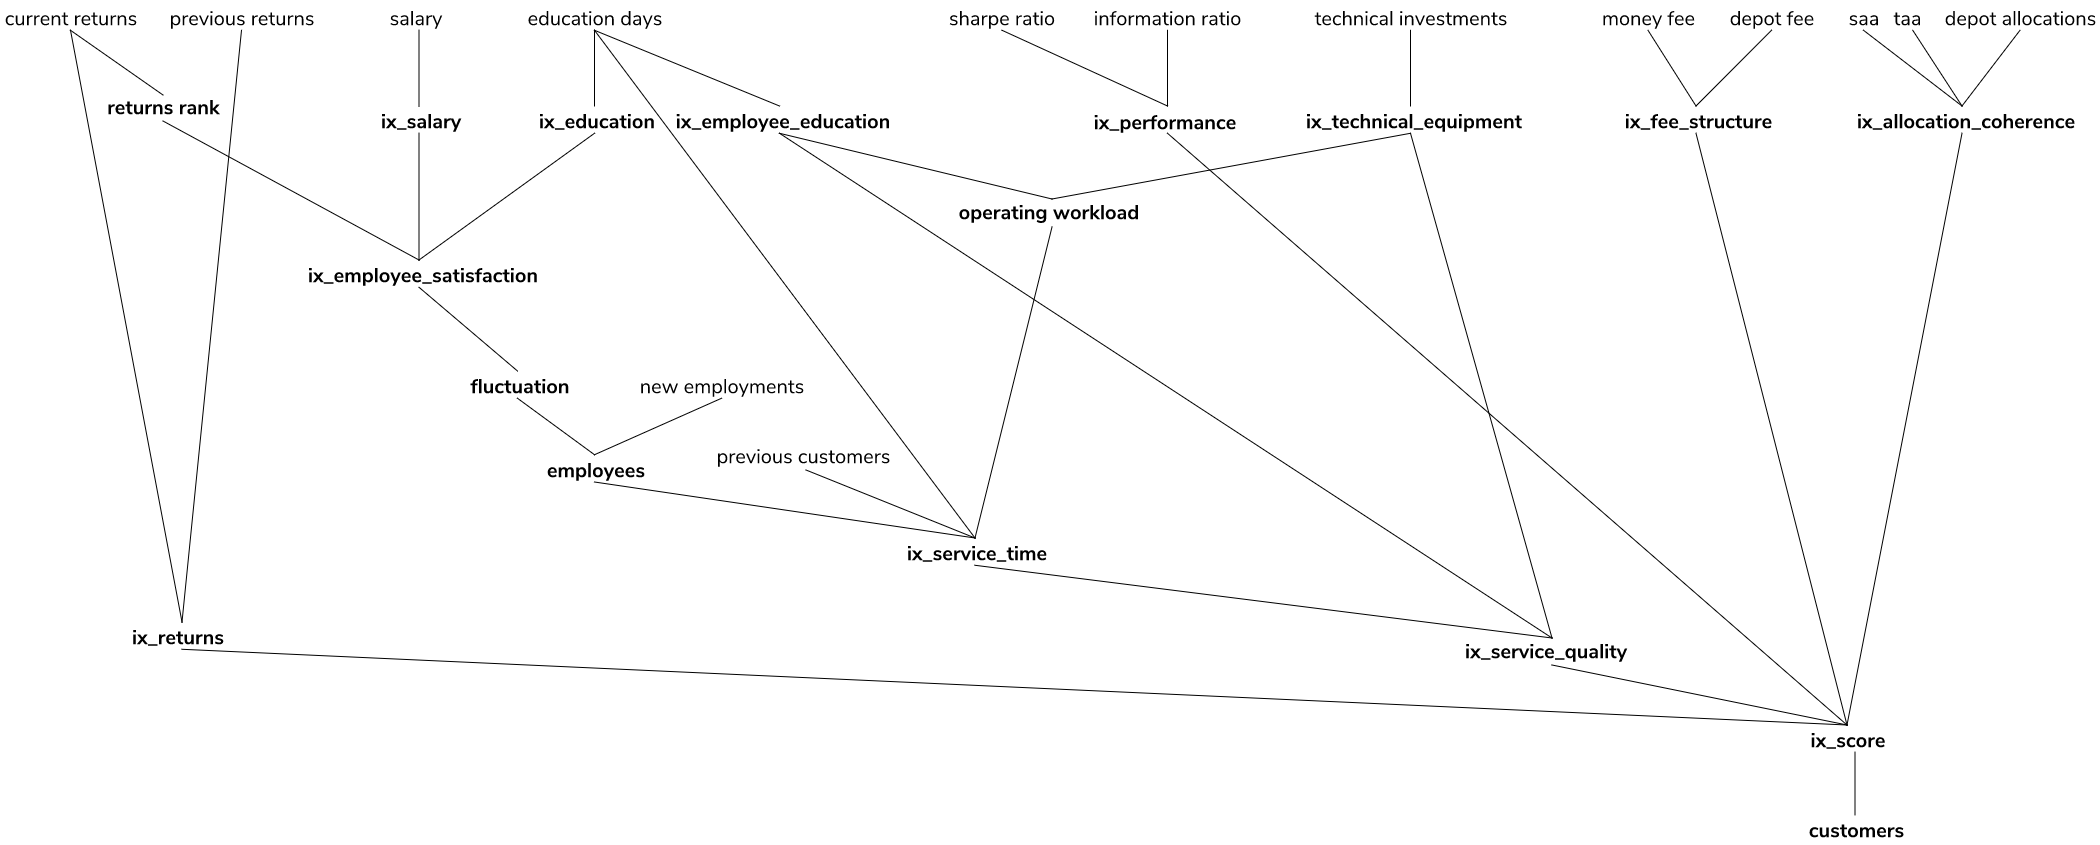
\includegraphics[width=\textwidth]{img/market_model_dependencies.png}
  \caption{Overview of market model dependencies; resolved from top-to-bottom with computed values in bold}
  \centering
  \label{fig:market_model_dependencies_full}
\end{sidewaysfigure}

\newpage

% ----------------------------------------
% Literaturverzeichnis
% ----------------------------------------
\selectlanguage{ngerman}
% \bibliography{bachelor_thesis}


\end{document}
